\chapter{Motion Control Design and Experimental Evaluation}
\label{chap:motion_control_design}

The high-level control loop is implemented in ROS2 inside the package
\texttt{sdpo\_motion\_control}. Its role is to compute planar velocity commands
for the omnidirectional robot from the measured pose and from the desired path.
The output of this layer is a body-frame velocity command:
\begin{equation}
    \mathbf{u}
    =
    \begin{bmatrix}
        v_x & v_y & \omega
    \end{bmatrix}^{T},
\end{equation}
where \(v_x\) is the linear velocity component along the robot \(x_b\)-axis,
  \(v_y\) is the linear velocity component along the robot \(y_b\)-axis, and
  \(\omega\) is the yaw rate around the vertical axis. Therefore, \(v_x\) and
  \(v_y\) are not two independent wheel speeds, but the two planar components of
  the robot velocity in the body frame.


The robot pose in the global frame is defined as:
\begin{equation}
    \mathbf{x}
    =
    \begin{bmatrix}
        x & y & \psi
    \end{bmatrix}^{T},
\end{equation}
where \(x\) and \(y\) are the robot position and \(\psi\) is the yaw angle. The
controllers studied in this section are structured path-following controllers.
They do not directly solve an optimization problem. Instead, they use geometric
quantities such as path projection, path tangent, cross-track error, and
along-track error.

Two controllers are analysed:

\begin{itemize}
    \item the \textbf{Moving Reference proportional controller}, implemented as
    \texttt{moving\_reference\_p};
    \item the \textbf{Linear Segment controller}, implemented as
    \texttt{linear\_segment}.
\end{itemize}

For each controller, the control law, the main parameters, the test setup, the
quantitative results, and the experimental figures are reported.

\section{Evaluation Protocol and Metrics}
\label{sec:evaluation_protocol}

The experiments are evaluated using the recorded path-following datasets stored
in:

\begin{itemize}
    \item \texttt{Test/test\_results/RECTANGULAR\_test/};
    \item \texttt{Test/test\_results/}.
\end{itemize}

The main performance indicators are computed from the sampled tracking errors.
For a generic error signal \(e_i\), with \(N\) samples, the root mean square
error is:

The root mean square errot is:
\begin{equation}
    \mathrm{RMSE}_{e}
    =
    \sqrt{
        \frac{1}{N}
        \sum_{i=1}^{N} e_i^2
    }.
\end{equation}

The mean absolute error is:
\begin{equation}
    \mathrm{MAE}_{e}
    =
    \frac{1}{N}
    \sum_{i=1}^{N} |e_i|.
\end{equation}

The maximum absolute error is:
\begin{equation}
    e_{\max}
    =
    \max_{i=1,\dots,N} |e_i|.
\end{equation}

The path progression ratio is used to understand how much of the reference path
was covered during the test:
\begin{equation}
    r_{\gamma}
    =
    \frac{\gamma_{\mathrm{final}}}{L_{\mathrm{path}}},
\end{equation}
where \(\gamma_{\mathrm{final}}\) is the final curvilinear abscissa reached by
the reference or projection point, and \(L_{\mathrm{path}}\) is the total path
length. A value close to one means that the robot completed almost the whole
path.

The velocity saturation ratios are also reported:
\begin{equation}
    r_{\mathrm{sat},v_x}, \quad
    r_{\mathrm{sat},v_y}, \quad
    r_{\mathrm{sat},\omega}.
\end{equation}
These values indicate the fraction of samples in which the corresponding
velocity command reached its imposed limit.

\section{Moving Reference Proportional Controller}
\label{sec:moving_reference_controller}

\subsection{Control Principle}

The Moving Reference controller tracks a virtual point that moves along the
path. The path is described by a parametric curve:
\begin{equation}
    \mathbf{p}_{r}(\gamma)
    =
    \begin{bmatrix}
        x_r(\gamma) \\
        y_r(\gamma)
    \end{bmatrix},
\end{equation}
where \(\gamma\) is the path coordinate. The reference point advances according
to:
\begin{equation}
    \dot{\gamma}
    =
    \mathrm{sat}
    \left(
        v_d + k_{\gamma} e_{\parallel},
        \dot{\gamma}_{\min},
        \dot{\gamma}_{\max}
    \right),
\end{equation}

where \(v_d\) is the desired path speed, \(k_{\gamma}\) is the progression gain,
and \(e_{\parallel}\) is the along-track error. The saturation function limits
the path progression between \(\dot{\gamma}_{\min}\) and
\(\dot{\gamma}_{\max}\).

The position error in the global frame is:
\begin{equation}
    \mathbf{e}_{w}
    =
    \mathbf{p}_{r}(\gamma)
    -
    \mathbf{p},
    \qquad
    \mathbf{p}
    =
    \begin{bmatrix}
        x \\
        y
    \end{bmatrix}.
\end{equation}

Since the robot receives velocity commands in its body frame, the error is
rotated using the yaw angle:
\begin{equation}
    \mathbf{e}_{b}
    =
    \mathbf{R}^{T}(\psi)
    \mathbf{e}_{w},
\end{equation}
with:
\begin{equation}
    \mathbf{R}(\psi)
    =
    \begin{bmatrix}
        \cos\psi & -\sin\psi \\
        \sin\psi & \cos\psi
    \end{bmatrix}.
\end{equation}

The proportional control law is:
\begin{equation}
    \begin{bmatrix}
        v_x \\
        v_y
    \end{bmatrix}
    =
    \begin{bmatrix}
        k_x e_{b,x} \\
        k_y e_{b,y}
    \end{bmatrix}.
\end{equation}

The heading is controlled independently with a proportional law:
\begin{equation}
    \omega
    =
    k_{\psi}
    e_{\psi},
\end{equation}
where:
\begin{equation}
    e_{\psi}
    =
    \mathrm{wrapToPi}(\psi_r - \psi).
\end{equation}
The function \(\mathrm{wrapToPi}(\cdot)\) maps an angle into the interval
  \([-\pi,\pi]\). This is necessary because yaw angles are periodic, in this case the controller always uses the shortest angular error

Finally, the command is saturated to respect the velocity limits:
\begin{equation}
    v_x \in [-v_{x,\max}, v_{x,\max}],
    \quad
    v_y \in [-v_{y,\max}, v_{y,\max}],
    \quad
    \omega \in [-\omega_{\max}, \omega_{\max}].
\end{equation}

This controller is simple and robust, but its performance strongly depends on
the balance between the path progression speed and the feedback gains. If the
virtual point moves too fast, the robot follows the path with a delay. If it
moves too slowly, the robot can track accurately but the test becomes slower.

\subsection{Test Parameters and Results}

\noindent
  \textbf{Test legend:}
  \begin{itemize}
      \item \textbf{MR-R01}: \texttt{PF\_2026-04-27\_RECT\_MAP\_MREFP\_V01\_R01};
      \item \textbf{P-R01}: \texttt{PF\_2026-04-27\_RECT\_MAP\_PONLY\_V01\_R01};
      \item \textbf{P-R02}: \texttt{PF\_2026-04-27\_RECT\_MAP\_PONLY\_V01\_R02}.
\end{itemize}

\begin{table}[H]
  \centering
  \caption{Moving Reference controller: main test parameters.}
  \label{tab:mref_parameters}
  \small
  \begin{tabular}{lccc}
  \toprule
  \textbf{Parameter} &
  \textbf{MR-R01} &
  \textbf{P-R01} &
  \textbf{P-R02} \\
  \midrule
  Path & RECT & RECT & RECT \\
  Frame & MAP & MAP & MAP \\
  Controller mode & \texttt{moving\_reference\_p} & \texttt{moving\_reference\_p} & \texttt{moving\_reference\_p} \\
  Heading mode & fixed & fixed & fixed \\
  \(v_d\) [m/s] & 0.35 & 0.35 & 0.35 \\
  \(k_{\gamma}\) & 0.50 & 0.50 & 0.50 \\
  \(\dot{\gamma}_{\min}\) [m/s] & 0.10 & 0.10 & 0.10 \\
  \(\dot{\gamma}_{\max}\) [m/s] & 0.35 & 0.35 & 0.35 \\
  Control rate [Hz] & 50 & 50 & 50 \\
  \(kp_{x}\) & 0.50 & 0.80 & 0.50 \\
  \(kp_{y}\) & 0.60 & 0.90 & 0.50 \\
  \(kp_{yaw}\) & 0.50 & 0.50 & 0.50 \\
  \(v_{x,\max}\) [m/s] & 0.40 & 0.40 & 0.40 \\
  \(v_{y,\max}\) [m/s] & 0.40 & 0.40 & 0.40 \\
  \(\omega_{\max}\) [rad/s] & 0.35 & 0.35 & 0.35 \\
  \bottomrule
  \end{tabular}
\end{table}

\begin{table}[H]
  \centering
  \caption{Moving Reference controller: experimental results.}
  \label{tab:mref_experimental_results}
  \small
  \begin{tabular}{lccc}
  \toprule
  \textbf{Metric} &
  \textbf{MR-R01} &
  \textbf{P-R01} &
  \textbf{P-R02} \\
  \midrule
  Duration [s] & 30.56 & 16.12 & 16.28 \\
  Samples & 975 & 515 & 514 \\
  Mean sample time [s] & 0.0314 & 0.0314 & 0.0317 \\
  Real path length [m] & 8.1990 & 4.9195 & 4.7319 \\
  Final \(\gamma\) [m] & 1.5230 & 0.6813 & 2.9163 \\
  Path progress ratio \(r_{\gamma}\) & 0.3626 & 0.1622 & 0.6944 \\
  \(\mathrm{RMSE}_x\) [m] & 0.0509 & 0.0455 & 0.0556 \\
  \(\mathrm{RMSE}_y\) [m] & 0.1021 & 0.0930 & 0.0609 \\
  \(\mathrm{RMSE}_{\psi}\) [rad] & 0.0141 & 0.0148 & 0.0147 \\
  \(\mathrm{RMSE}_{e_{\parallel}}\) [m] & 0.0701 & 0.0629 & 0.0772 \\
  \(\mathrm{MAE}_{e_{\parallel}}\) [m] & 0.0593 & 0.0548 & 0.0704 \\
  \(\max |e_{\parallel}|\) [m] & 0.1163 & 0.1124 & 0.1190 \\
  \(\mathrm{IAE}_{e_{\parallel}}\) & 1.8162 & 0.8878 & 1.1433 \\
  \(\max |e_{\psi}|\) [rad] & 0.0344 & 0.0447 & 0.0304 \\
  Saturation ratio \(v_x\) & 0.00 & 0.00 & 0.00 \\
  Saturation ratio \(v_y\) & 0.00 & 0.00 & 0.00 \\
  Saturation ratio \(\omega\) & 0.00 & 0.00 & 0.00 \\
  \bottomrule
  \end{tabular}
\end{table}

\begin{figure}[H]
    \centering
    \begin{subfigure}{\textwidth}
        \centering
        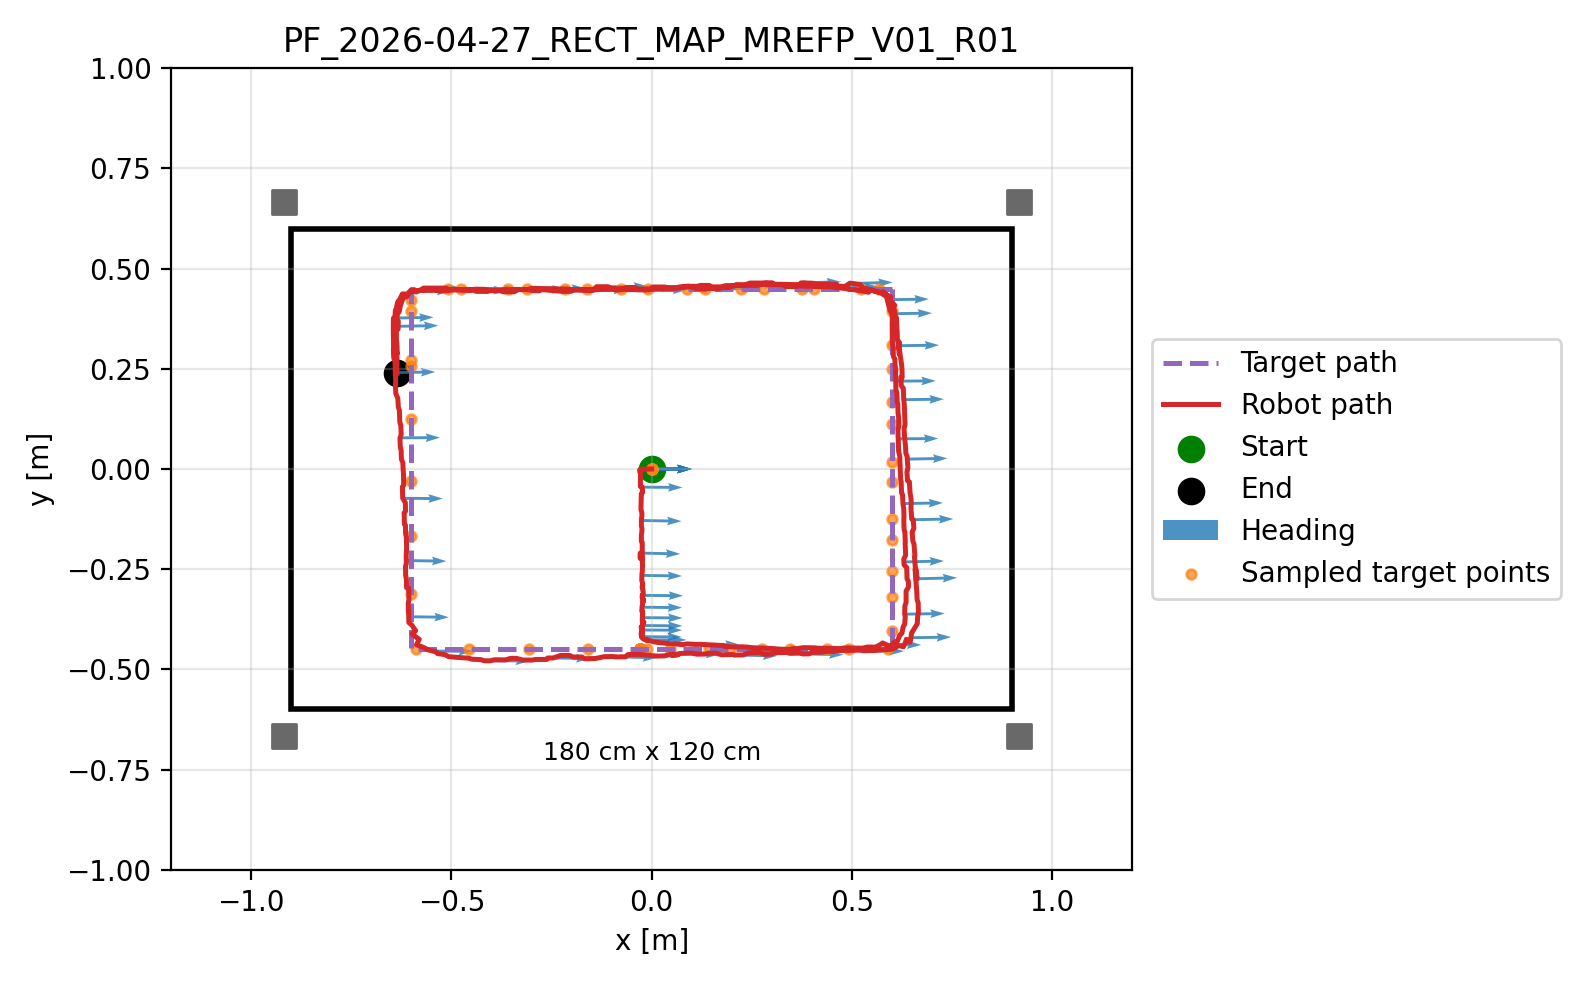
\includegraphics[width=0.7\linewidth]{IMG/controller/MREFP/MR_R01_xy_map.png}
        \caption{MR\_R01 xy map}
        \label{fig:MR_R01_xy_map}
    \end{subfigure}

    \vspace{0.2em}

    \begin{subfigure}{\textwidth}
        \centering
        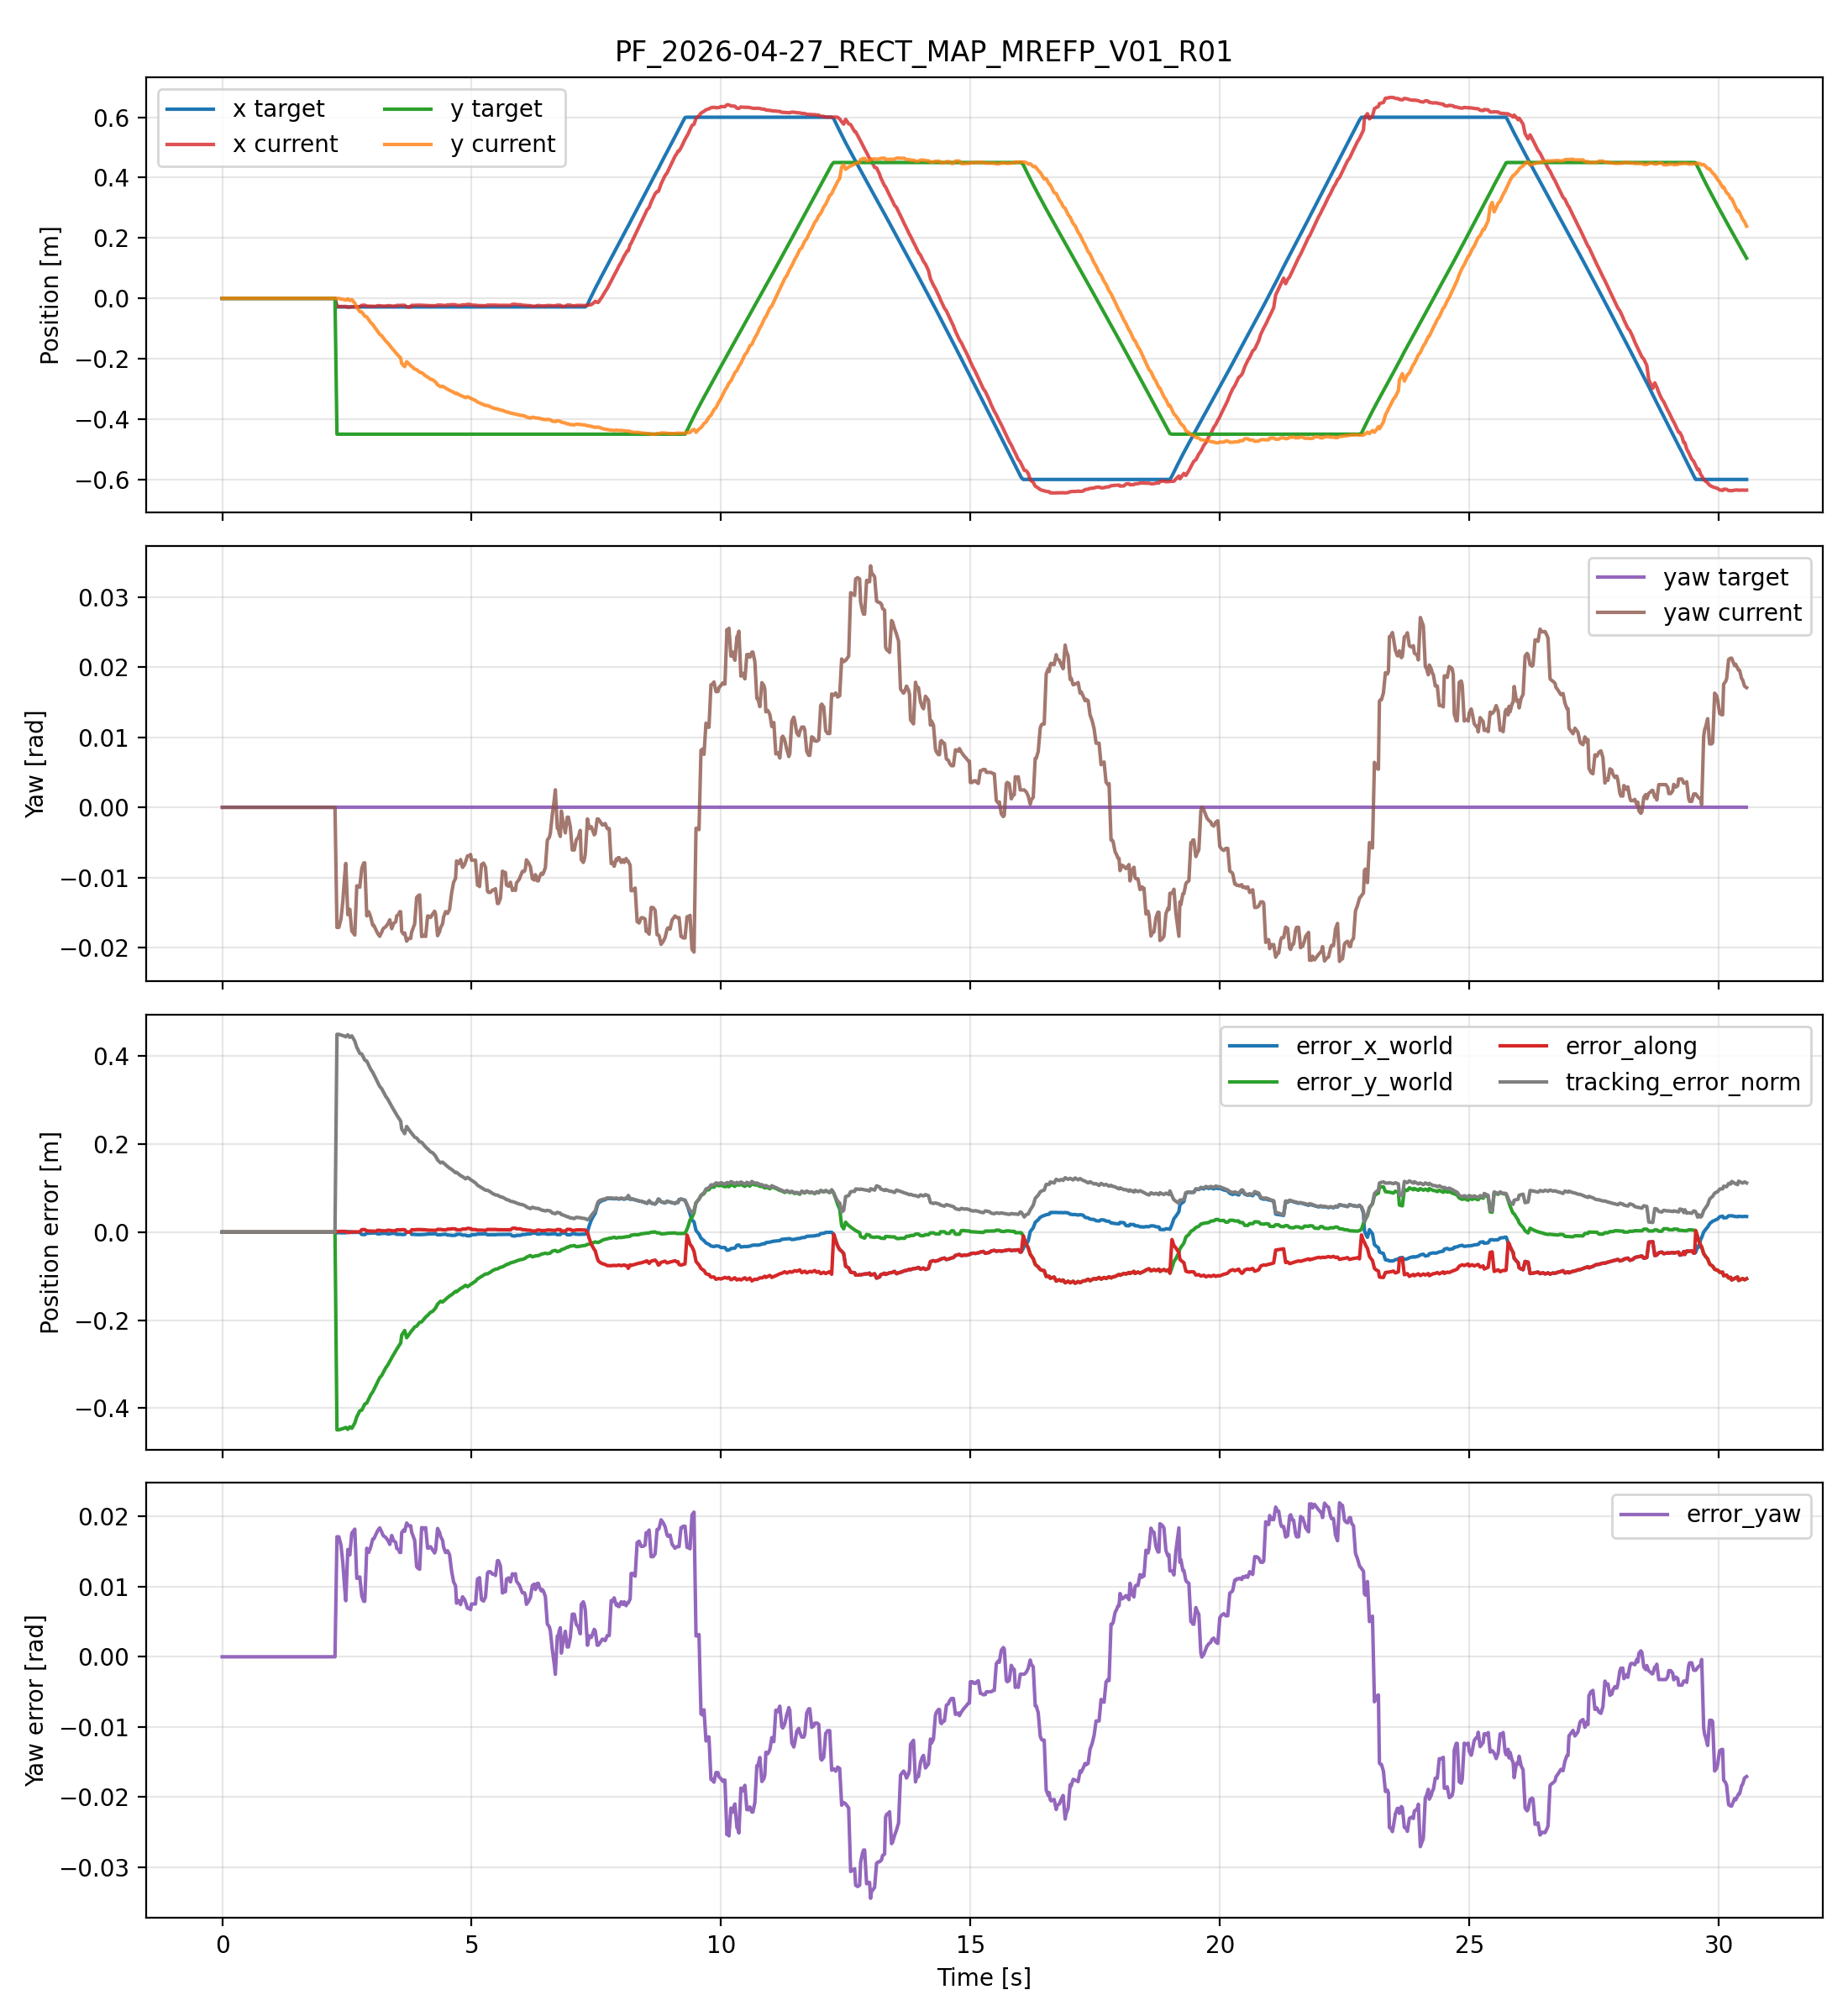
\includegraphics[width=0.6\linewidth]{IMG/controller/MREFP/MR_R01_target_tracking_and_errors.png}
        \caption{MR\_R01 tracking and errors}
        \label{fig:MR_R01_tracking_and_errors}
    \end{subfigure}
    
    \vspace{0.2em}
    \caption{Experimental results for MR\_R01 scenario.} 
    \label{fig:MR_R01_general}
\end{figure}

\newpage
\begin{figure}[H]
    \centering
    \begin{subfigure}{\textwidth}
        \centering
        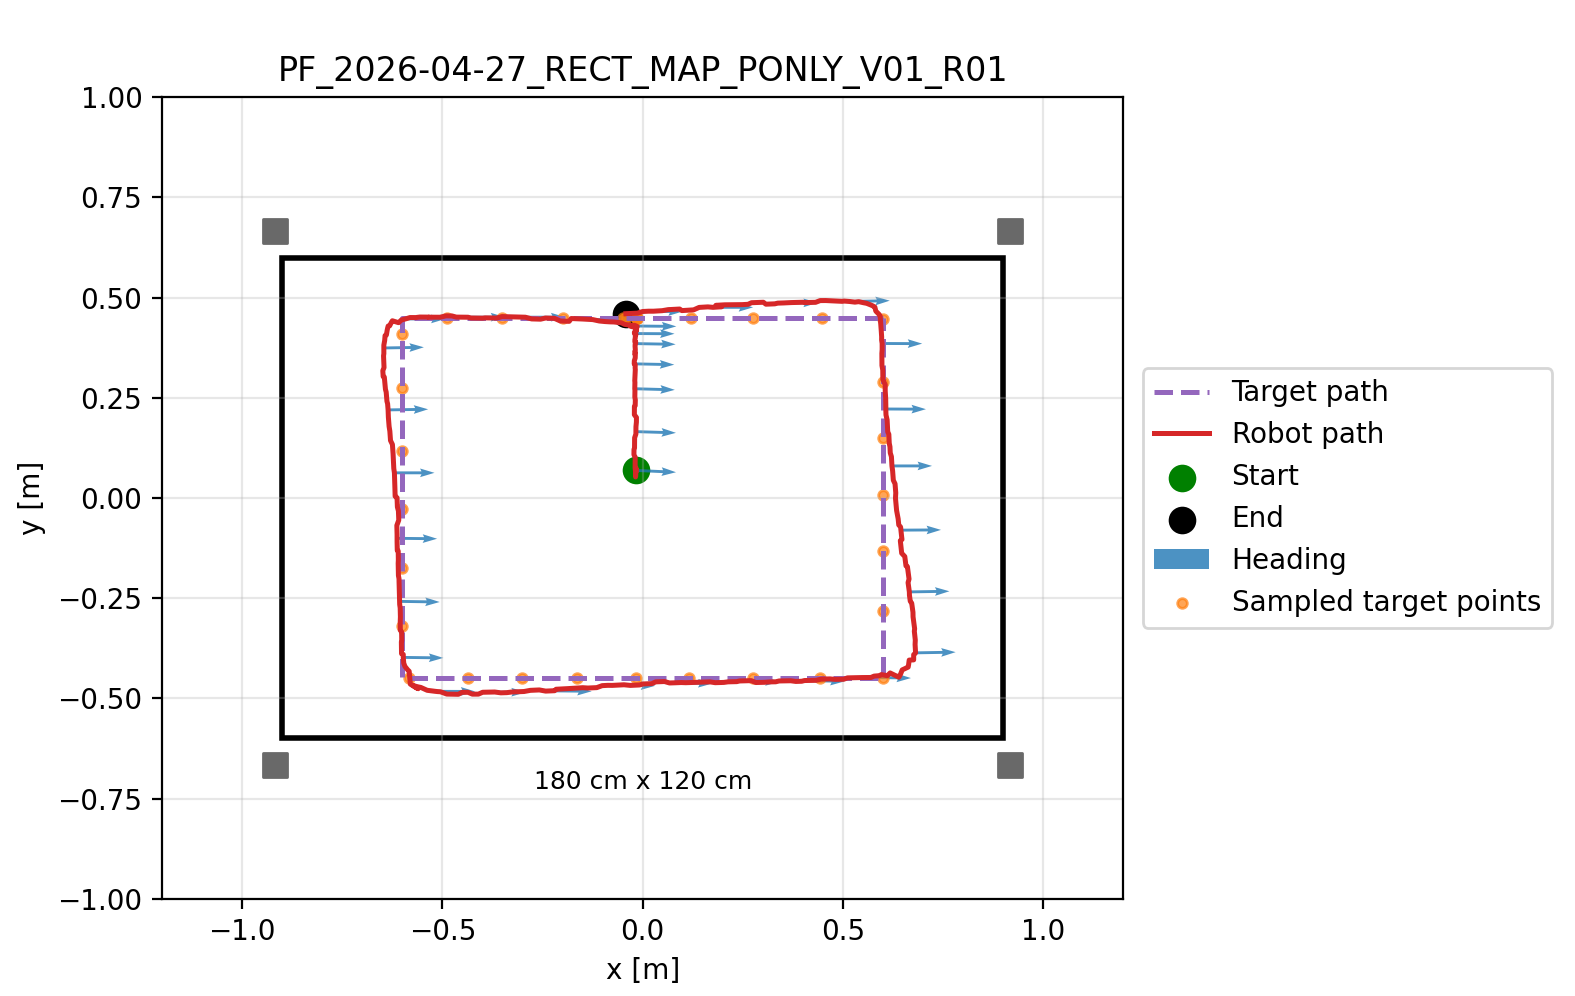
\includegraphics[width=0.7\linewidth]{IMG/controller/MREFP/PR01_xy_map.png}
        \caption{P\_R01 xy map}
        \label{fig:PR01_xy_map}
    \end{subfigure}

    \vspace{0.2em}

    \begin{subfigure}{\textwidth}
        \centering
        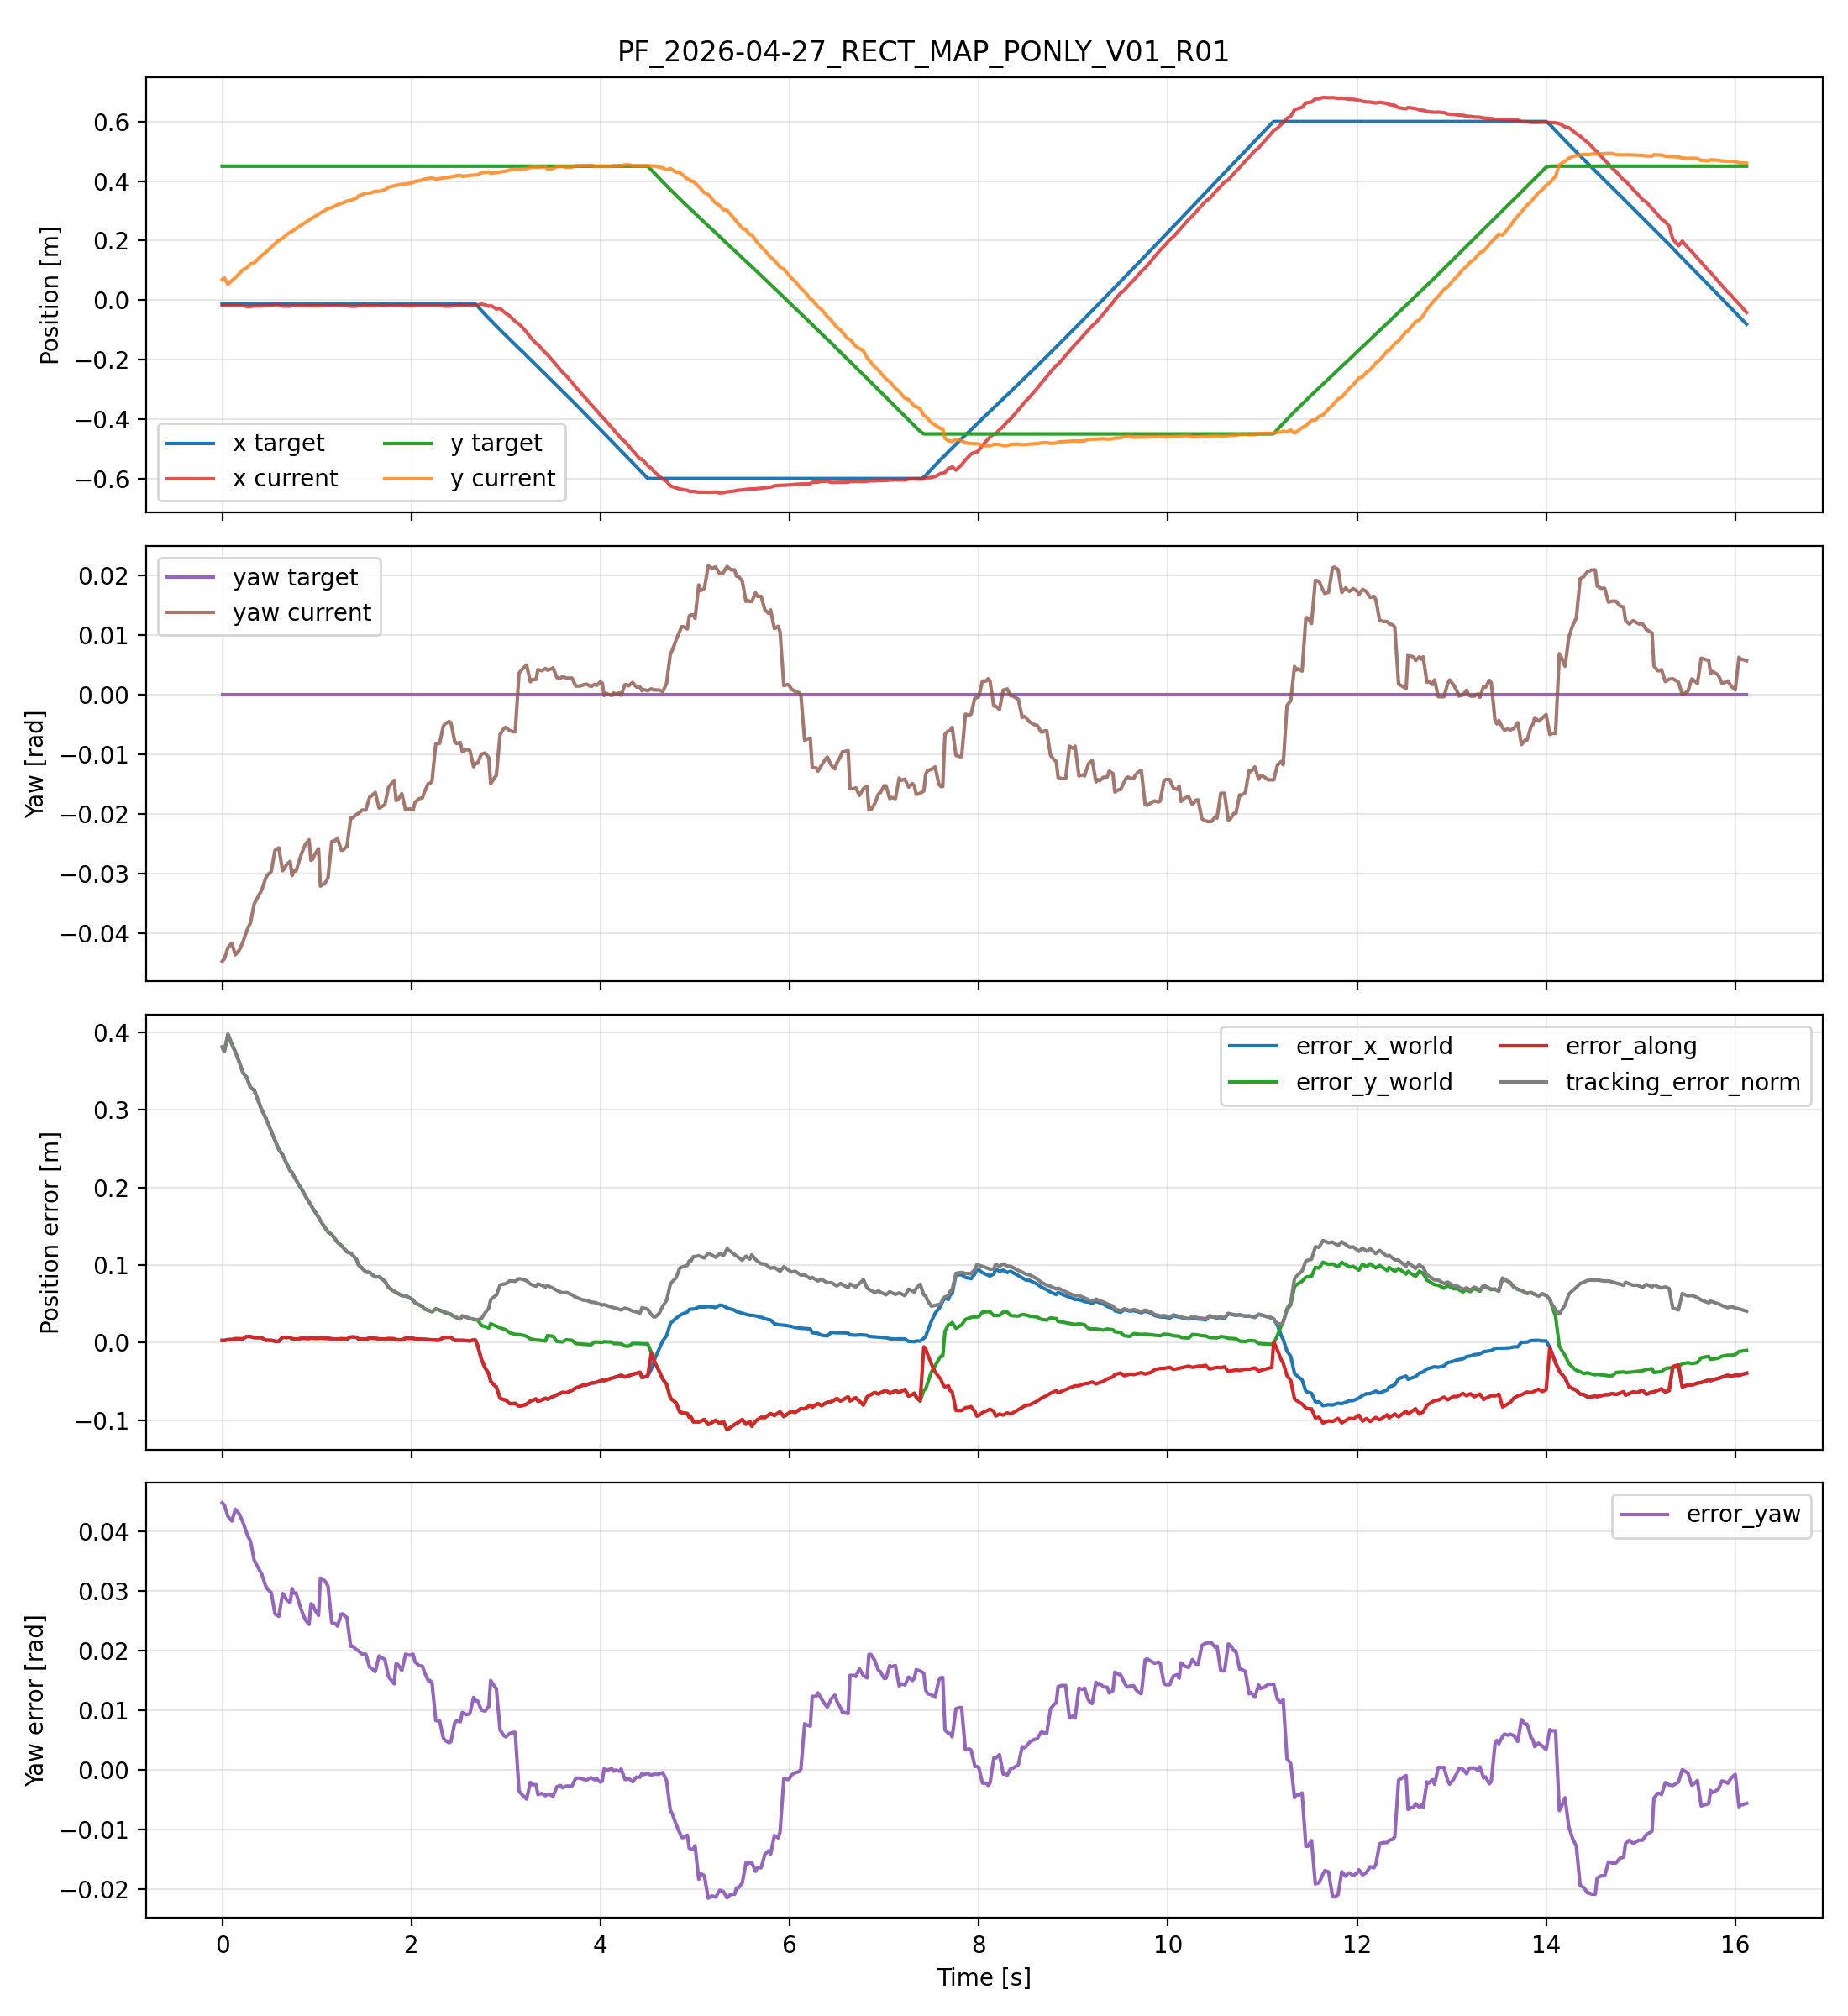
\includegraphics[width=0.7\linewidth]{IMG/controller/MREFP/PR01_target_tracking_and_errors.png}
        \caption{P\_R01 tracking and errors}
        \label{fig:PR01_tracking_and_errors}
    \end{subfigure}
    
    \vspace{0.2em}
    \caption{Experimental results for P\_R01 scenario.} 
    \label{fig:PR01_general}
\end{figure}

\newpage
\begin{figure}[H]
    \centering
    \begin{subfigure}{\textwidth}
        \centering
        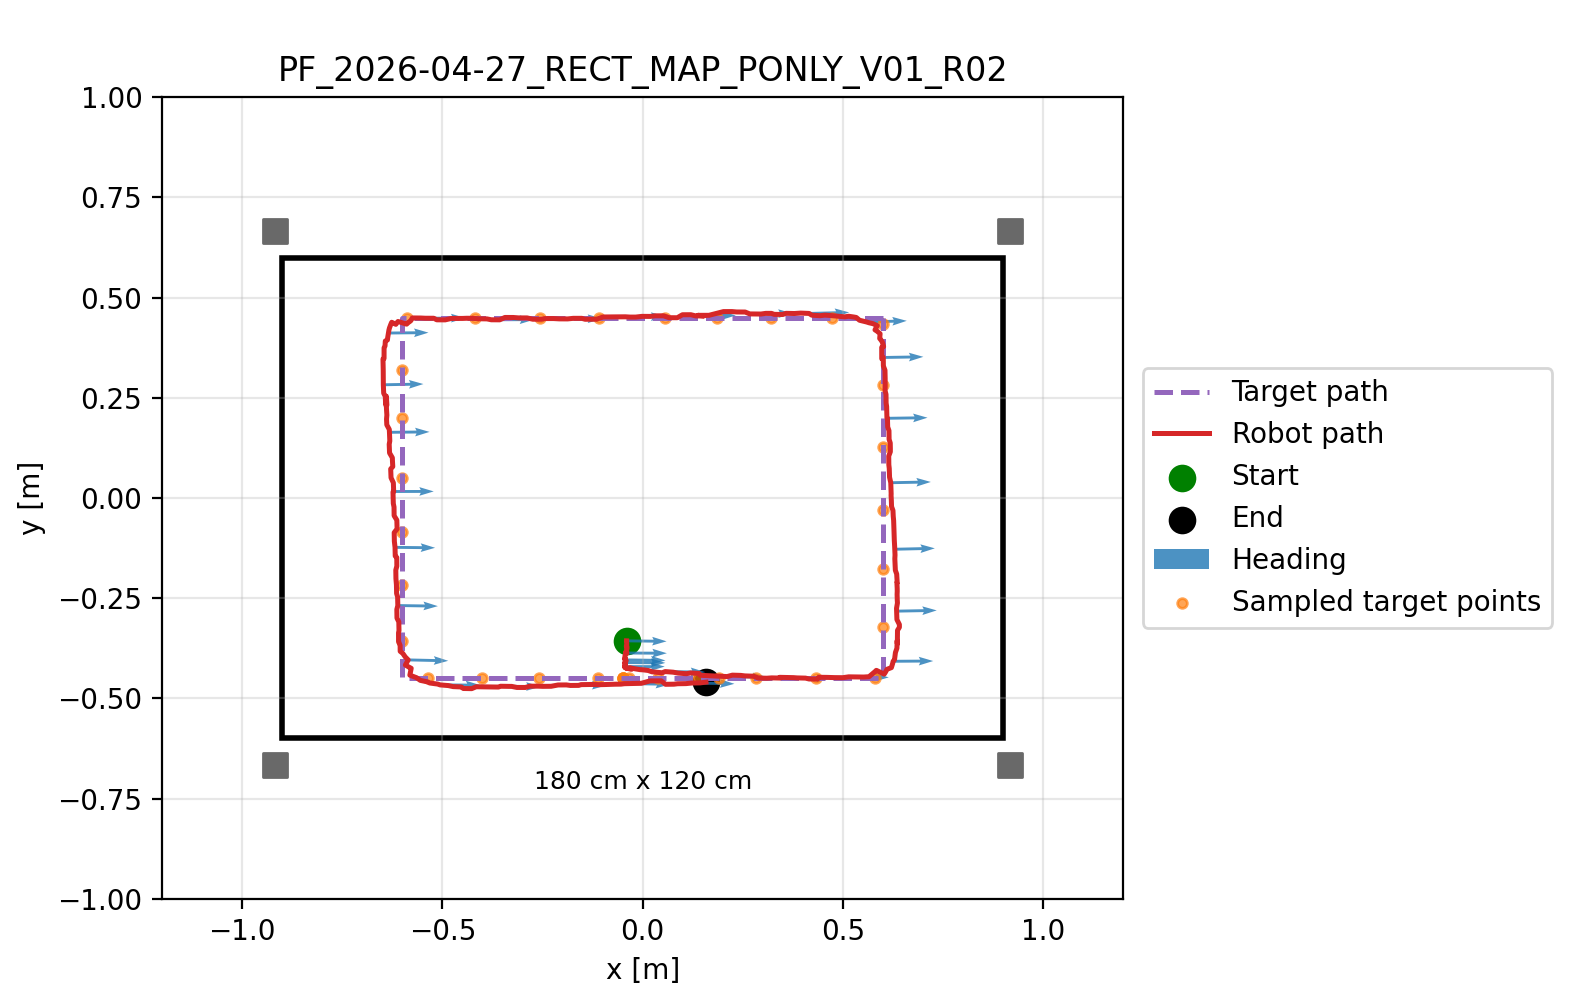
\includegraphics[width=0.7\linewidth]{IMG/controller/MREFP/PR02_xy_map.png}
        \caption{P\_R02 xy map}
        \label{fig:PR02_xy_map}
    \end{subfigure}

    \vspace{0.2em}

    \begin{subfigure}{\textwidth}
        \centering
        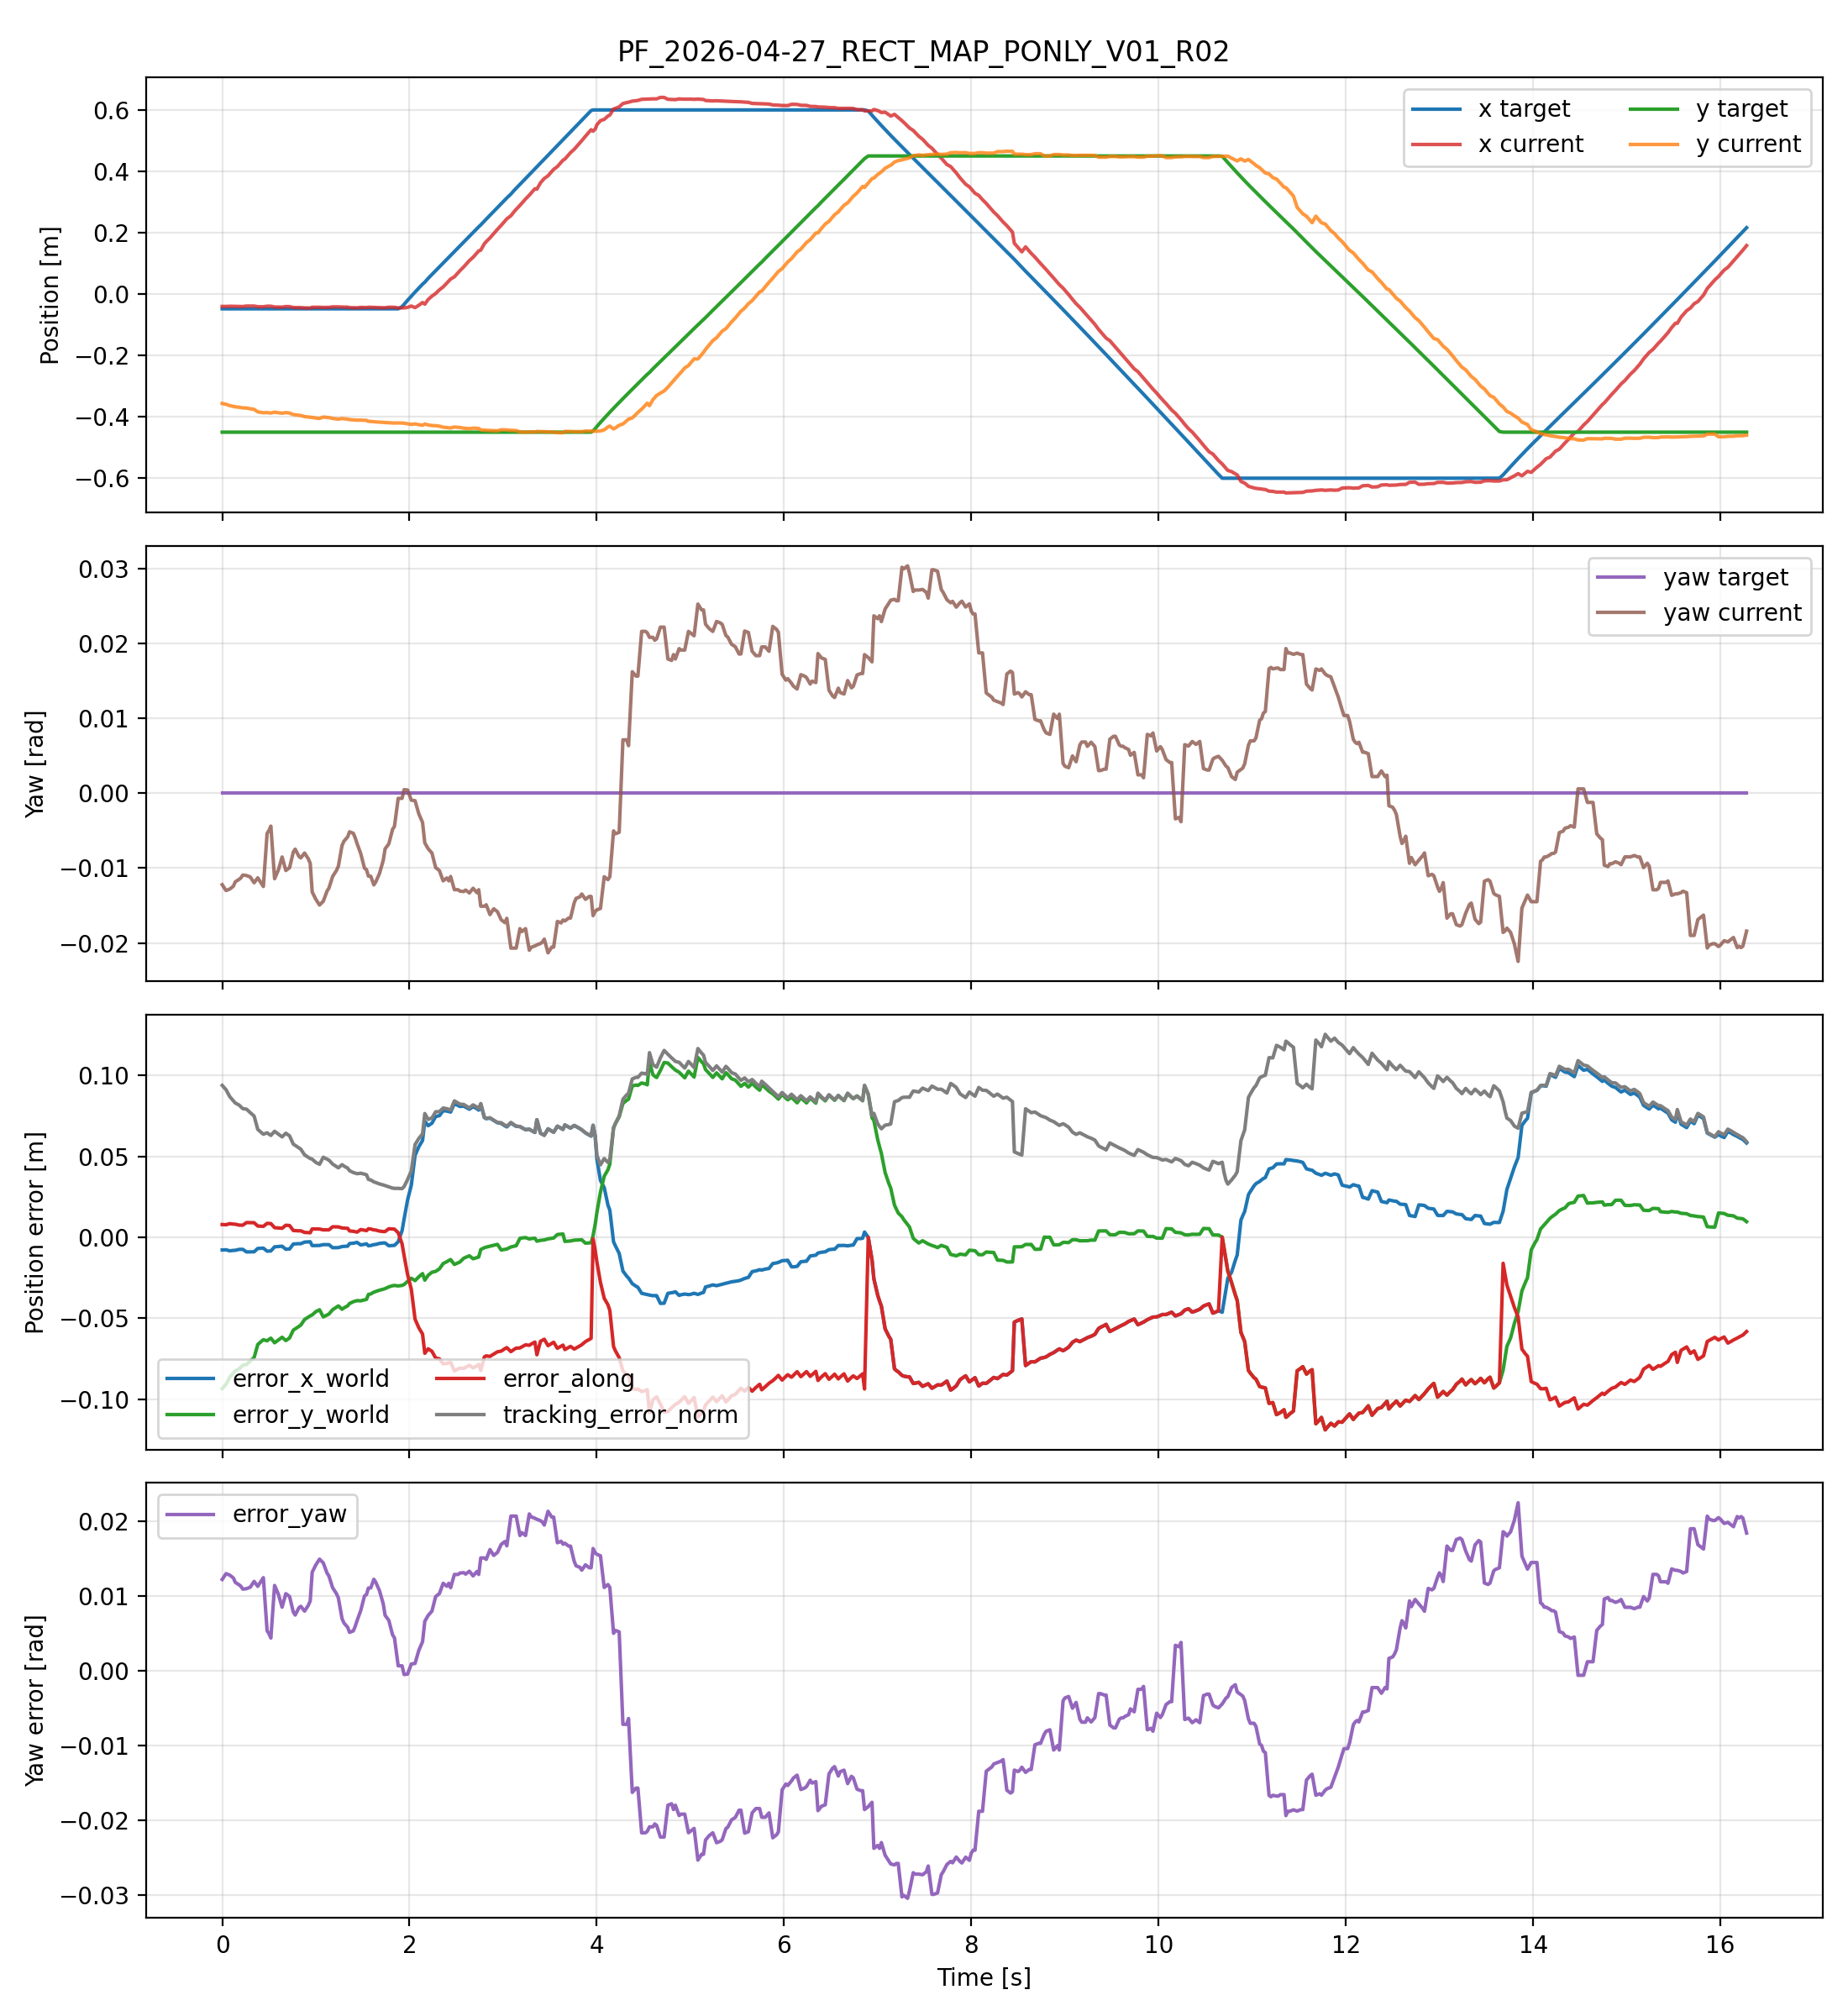
\includegraphics[width=0.7\linewidth]{IMG/controller/MREFP/PR02_target_tracking_and_errors.png}
        \caption{P\_R02 tracking and errors}
        \label{fig:PR02_tracking_and_errors}
    \end{subfigure}
    
    \vspace{0.2em}
    \caption{Experimental results for P\_R02 scenario.} 
    \label{fig:PR01_general}
\end{figure}

\section{Linear Segment Controller}
\subsection{Control Principle}

The Linear Segment controller uses the local geometry of the path. At each
control step, the robot position is projected onto the current path segment.
Given two consecutive path points:
\begin{equation}
    \mathbf{p}_i
    =
    \begin{bmatrix}
        x_i \\
        y_i
    \end{bmatrix},
    \qquad
    \mathbf{p}_{i+1}
    =
    \begin{bmatrix}
        x_{i+1} \\
        y_{i+1}
    \end{bmatrix},
\end{equation}
the segment vector is:
\begin{equation}
    \mathbf{s}_i
    =
    \mathbf{p}_{i+1}
    -
    \mathbf{p}_i.
\end{equation}

The unit tangent vector is:
\begin{equation}
    \mathbf{t}_i
    =
    \frac{\mathbf{s}_i}{\|\mathbf{s}_i\|}.
\end{equation}

The normal vector is obtained by rotating the tangent by \(90^\circ\):
\begin{equation}
    \mathbf{n}_i
    =
    \begin{bmatrix}
        -t_{i,y} \\
        t_{i,x}
    \end{bmatrix}.
\end{equation}

The projection coefficient is:
\begin{equation}
    \alpha
    =
    \frac{
        (\mathbf{p} - \mathbf{p}_i)^T \mathbf{s}_i
    }{
        \mathbf{s}_i^T \mathbf{s}_i
    }.
\end{equation}

To keep the projected point inside the segment, \(\alpha\) is limited:
\begin{equation}
    \alpha_c
    =
    \mathrm{sat}(\alpha,0,1).
\end{equation}

The closest point on the segment is:
\begin{equation}
    \mathbf{p}_{c}
    =
    \mathbf{p}_i
    +
    \alpha_c \mathbf{s}_i.
\end{equation}

The position error is:
\begin{equation}
    \mathbf{e}
    =
    \mathbf{p}_{c}
    -
    \mathbf{p}.
\end{equation}

This error is decomposed into an along-track component and a lateral component:
\begin{equation}
    e_{\parallel}
    =
    \mathbf{e}^{T}\mathbf{t}_i,
    \qquad
    e_{\perp}
    =
    \mathbf{e}^{T}\mathbf{n}_i.
\end{equation}

The desired velocity in the world frame is:
\begin{equation}
    \mathbf{v}_{w}
    =
    v_d \mathbf{t}_i
    +
    k_{\parallel} e_{\parallel} \mathbf{t}_i
    +
    k_{\perp} e_{\perp} \mathbf{n}_i.
\end{equation}

The first term moves the robot along the path. The second term corrects the
longitudinal error. The third term corrects the lateral error and is the main
term used to reduce the cross-track deviation.

Since the robot command is expressed in body frame, the world-frame velocity is
rotated using:
\begin{equation}
    \mathbf{v}_{b}
    =
    \mathbf{R}^{T}(\psi)
    \mathbf{v}_{w}.
\end{equation}

Therefore:
\begin{equation}
    v_x = v_{b,x},
    \qquad
    v_y = v_{b,y}.
\end{equation}

The yaw motion is controlled separately:
\begin{equation}
    \omega
    =
    k_{\psi}
    \mathrm{wrapToPi}(\psi_r - \psi).
\end{equation}

This formulation is useful for an omnidirectional robot because longitudinal
motion and lateral correction can be commanded at the same time. For this
reason, the robot does not need to align its body with the path before reducing
the lateral error.

\subsection{Test Parameters}

\noindent
  \textbf{Test legend:}
  \begin{itemize}
      \item \textbf{LIN-01}: \texttt{PF\_2026-04-28\_INFIN\_MAP\_LINEAR\_V01\_R01};
      \item \textbf{LIN-02}: \texttt{PF\_2026-04-29\_INFIN\_MAP\_LINEAR\_V01\_R02};
      \item \textbf{LIN-03}: \texttt{PF\_2026-04-29\_INFIN\_MAP\_LINEAR\_V01\_R07};
      \item \textbf{LIN-04}: \texttt{PF\_2026-04-29\_INFIN\_MAP\_LINEAR\_V01\_R08};
      \item \textbf{LIN-05}: \texttt{PF\_2026-04-29\_INFIN\_MAP\_LINEAR\_V01\_R10}.
  \end{itemize}

  \begin{table}[H]
  \centering
  \caption{Linear Segment controller: configuration parameters of the selected tests.}
  \label{tab:linear_configuration_parameters}
  \small
  \begin{tabular}{lccccc}
  \toprule
  \textbf{Parameter} &
  \textbf{LIN-01} &
  \textbf{LIN-02} &
  \textbf{LIN-03} &
  \textbf{LIN-04} &
  \textbf{LIN-05} \\
  \midrule
  Path & INFIN & INFIN & INFIN & INFIN & INFIN \\
  Frame & MAP & MAP & MAP & MAP & MAP \\
  Heading mode & fixed & fixed & fixed & fixed & fixed \\
  \(v_d\) [m/s] & 0.35 & 0.20 & 0.30 & 0.40 & 0.50 \\
  \(k_{\gamma}\) & 0.20 & 0.20 & 0.20 & 0.30 & 0.40 \\
  \(\dot{\gamma}_{\min}\) [m/s] & 0.10 & 0.05 & 0.05 & 0.05 & 0.05 \\
  \(\dot{\gamma}_{\max}\) [m/s] & 0.35 & 0.20 & 0.20 & 0.30 & 0.30 \\
  \(k_{\parallel}\) & 0.00 & 0.40 & 1.00 & 1.00 & 1.00 \\
  \(k_{\perp}\) & 0.80 & 3.00 & 5.00 & 5.00 & 8.00 \\
  Control rate [Hz] & 50 & 50 & 50 & 50 & 50 \\
  \bottomrule
  \end{tabular}
  \end{table}

  \begin{table}[H]
  \centering
  \caption{Linear Segment controller: experimental results of the selected tests.}
  \label{tab:linear_experimental_results}
  \small
  \begin{tabular}{lccccc}
  \toprule
  \textbf{Metric} &
  \textbf{LIN-01} &
  \textbf{LIN-02} &
  \textbf{LIN-03} &
  \textbf{LIN-04} &
  \textbf{LIN-05} \\
  \midrule
  Duration [s] & 23.80 & 39.20 & 32.28 & 27.39 & 22.58 \\
  Samples & 753 & 1268 & 1020 & 853 & 716 \\
  Mean sample time [s] & 0.0316 & 0.0309 & 0.0317 & 0.0321 & 0.0316 \\
  Real path length [m] & 7.7631 & 7.7922 & 9.6978 & 10.7535 & 11.6237 \\
  Final \(\gamma\) [m] & 2.0687 & 4.4860 & 2.0970 & 2.1181 & 2.1832 \\
  Path progress ratio \(r_{\gamma}\) & 0.4542 & 0.9849 & 0.4604 & 0.4650 & 0.4793 \\
  \(\mathrm{RMSE}_x\) [m] & 0.0720 & 0.0125 & 0.0172 & 0.0270 & 0.0396 \\
  \(\mathrm{RMSE}_y\) [m] & 0.0586 & 0.0113 & 0.0148 & 0.0228 & 0.0252 \\
  \(\mathrm{RMSE}_{\psi}\) [rad] & 0.0139 & 0.0082 & 0.0120 & 0.0187 & 0.0324 \\
  \(\mathrm{RMSE}_{e_{\parallel}}\) [m] & 0.0028 & 0.0003 & 0.0005 & 0.0005 & 0.0009 \\
  \(\mathrm{MAE}_{e_{\parallel}}\) [m] & 0.0009 & 0.00005 & 0.00008 & 0.00010 & 0.00020 \\
  \(\max |e_{\parallel}|\) [m] & 0.0217 & 0.0037 & 0.0049 & 0.0057 & 0.0104 \\
  \(\mathrm{IAE}_{e_{\parallel}}\) & 0.0206 & 0.0020 & 0.0025 & 0.0027 & 0.0044 \\
  \(\max |e_{\psi}|\) [rad] & 0.0340 & 0.0264 & 0.0310 & 0.0464 & 0.0745 \\
  Saturation ratio \(v_x\) & 0.0000 & 0.0000 & 0.0186 & 0.0668 & 0.2304 \\
  Saturation ratio \(v_y\) & 0.0000 & 0.0000 & 0.0461 & 0.0961 & 0.1955 \\
  Saturation ratio \(\omega\) & 0.0000 & 0.0000 & 0.0000 & 0.0000 & 0.0000 \\
  \bottomrule
  \end{tabular}
  \end{table}

 The experimental validation analyzes the impact of varying desired speeds ($v_d$) and feedback gains ($k_{\parallel}, k_{\perp}$) on the Linear Segment controller. All tests were conducted on an "infinity" path within the MAP frame, utilizing a fixed-heading mode. The primary objective is to evaluate the trade-off between path progression, tracking accuracy, and control effort.

\paragraph{Baseline and Tuning Impact (LIN-01)}
The baseline configuration, \textbf{LIN-01} ($v_d = 0.35~\mathrm{m/s}$), employs a weak feedback action with $k_{\parallel}=0$ and $k_{\perp}=0.8$. This setup results in the poorest tracking performance among the selected runs:
\[
    \mathrm{RMSE}_x = 0.0720~\mathrm{m}, \quad \mathrm{RMSE}_y = 0.0586~\mathrm{m}, \quad \mathrm{RMSE}_{e_{\parallel}} = 0.0028~\mathrm{m}
\]
Since saturation ratios remain at zero, the high tracking error is not due to physical actuator limits but is directly attributable to the insufficient feedback gains, particularly the absence of longitudinal compensation ($k_{\parallel}=0$).

\paragraph{Optimal Performance (LIN-02)}
The most balanced results are achieved in \textbf{LIN-02}. By reducing the speed to $v_d = 0.20~\mathrm{m/s}$ and increasing the gains to $k_{\parallel}=0.4$ and $k_{\perp}=3.0$, the tracking errors decrease significantly:
\[
    \mathrm{RMSE}_x = 0.0125~\mathrm{m}, \quad \mathrm{RMSE}_y = 0.0113~\mathrm{m}, \quad \mathrm{RMSE}_{e_{\parallel}} = 0.0003~\mathrm{m}
\]
This configuration provides high path completion and negligible error without encountering velocity saturation, establishing a robust benchmark for reliable autonomous navigation.

\paragraph{High-Speed Scenarios and Actuator Limits (LIN-03 to LIN-05)}
As the desired speed increases, a clear degradation in performance and an increase in control effort are observed:

\begin{itemize}
    \item \textbf{LIN-03 ($v_d = 0.30~\mathrm{m/s}$):} Despite maintaining good local accuracy, the path progress ratio drops to $r_{\gamma} = 0.4604$. The controller begins to approach the actuation limits, with saturation ratios reaching $1.86\%$ on $v_x$ and $4.61\%$ on $v_y$.
    \item \textbf{LIN-04 ($v_d = 0.40~\mathrm{m/s}$):} The system nears its operational limits. Position errors and heading divergence increase ($\mathrm{RMSE}_{\psi} = 0.0187~\mathrm{rad}$), while saturation becomes more frequent ($r_{\mathrm{sat},v_y} \approx 9.61\%$).
    \item \textbf{LIN-05 ($v_d = 0.50~\mathrm{m/s}$):} In the fastest test, the controller hits significant saturation ($\approx 23\%$ on $v_x$). This prevents the full application of corrective commands, leading to the highest observed errors:
    \[
        \mathrm{RMSE}_x = 0.0396~\mathrm{m}, \quad \max |e_{\psi}| = 0.0745~\mathrm{rad}
    \]
\end{itemize}


\paragraph{Concluding Remarks}
The results demonstrate a direct correlation between target velocity and tracking stability. While \textbf{LIN-02} represents the ideal operational point for the current tuning, the high-speed tests highlight the physical and algorithmic boundaries of the system. To maintain accuracy at higher velocities, future developments should consider adaptive path progression or the introduction of feedforward terms to mitigate the lag induced by high-gain feedback during saturation.

\newpage
\begin{figure}[H]
    \centering
    \begin{subfigure}{\textwidth}
        \centering
        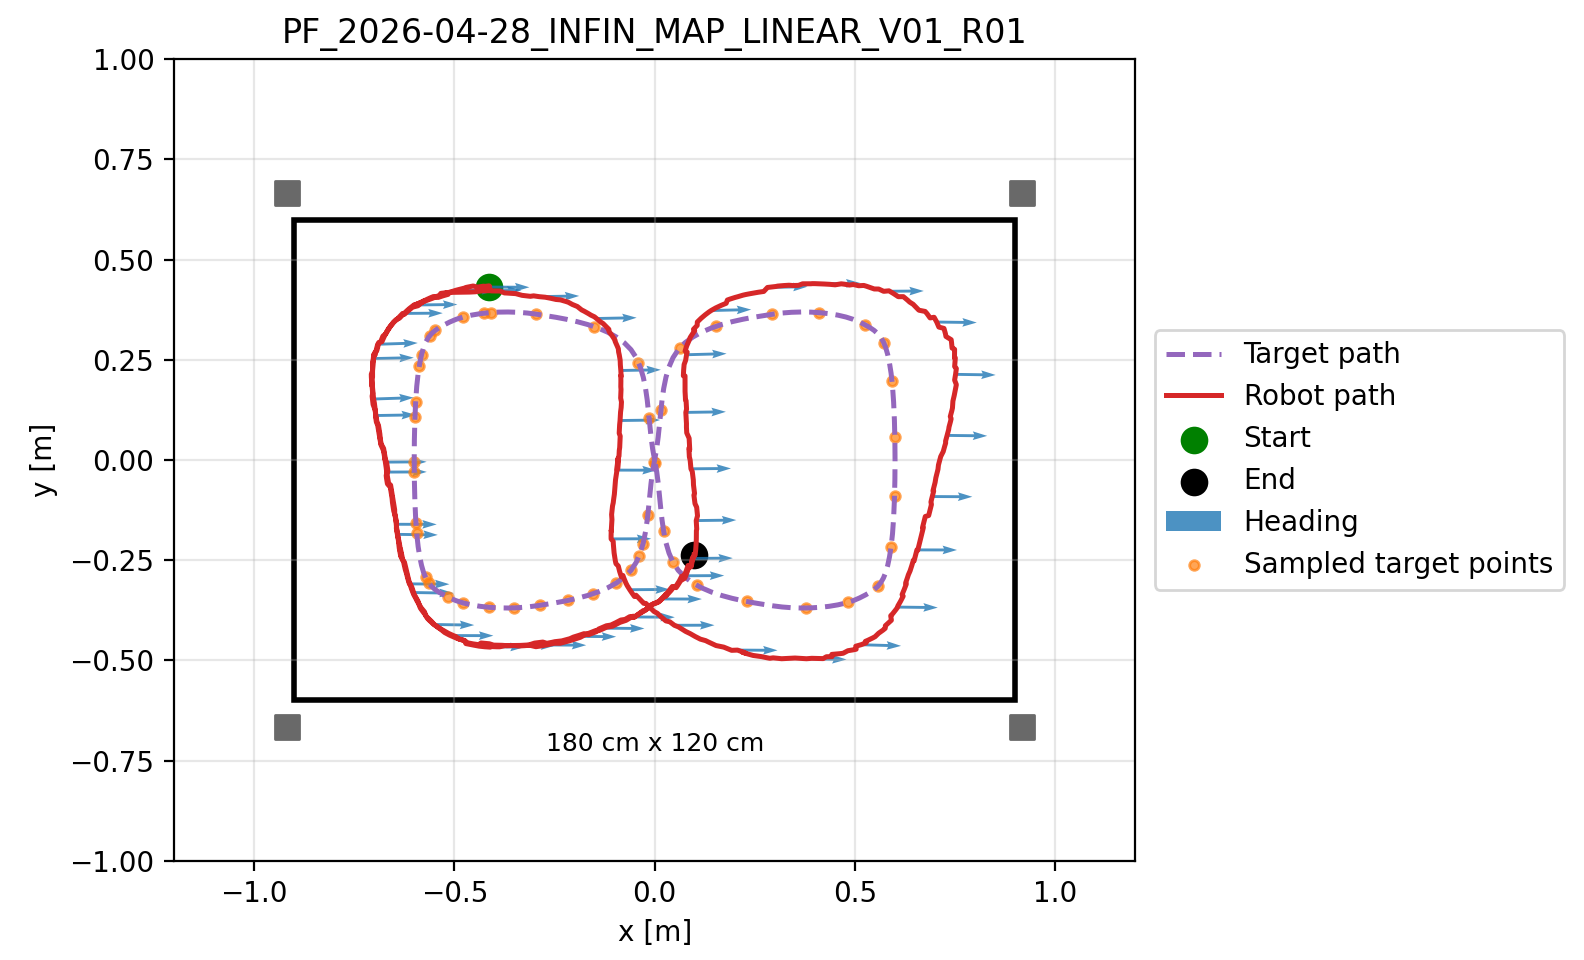
\includegraphics[width=0.7\linewidth]{IMG/controller/LIN/LIN_01_xy_map.png}
        \caption{LIN\_01 xy map}
        \label{fig:LIN_01_xy_map}
    \end{subfigure}

    \vspace{0.5em}

    \begin{subfigure}{\textwidth}
        \centering
        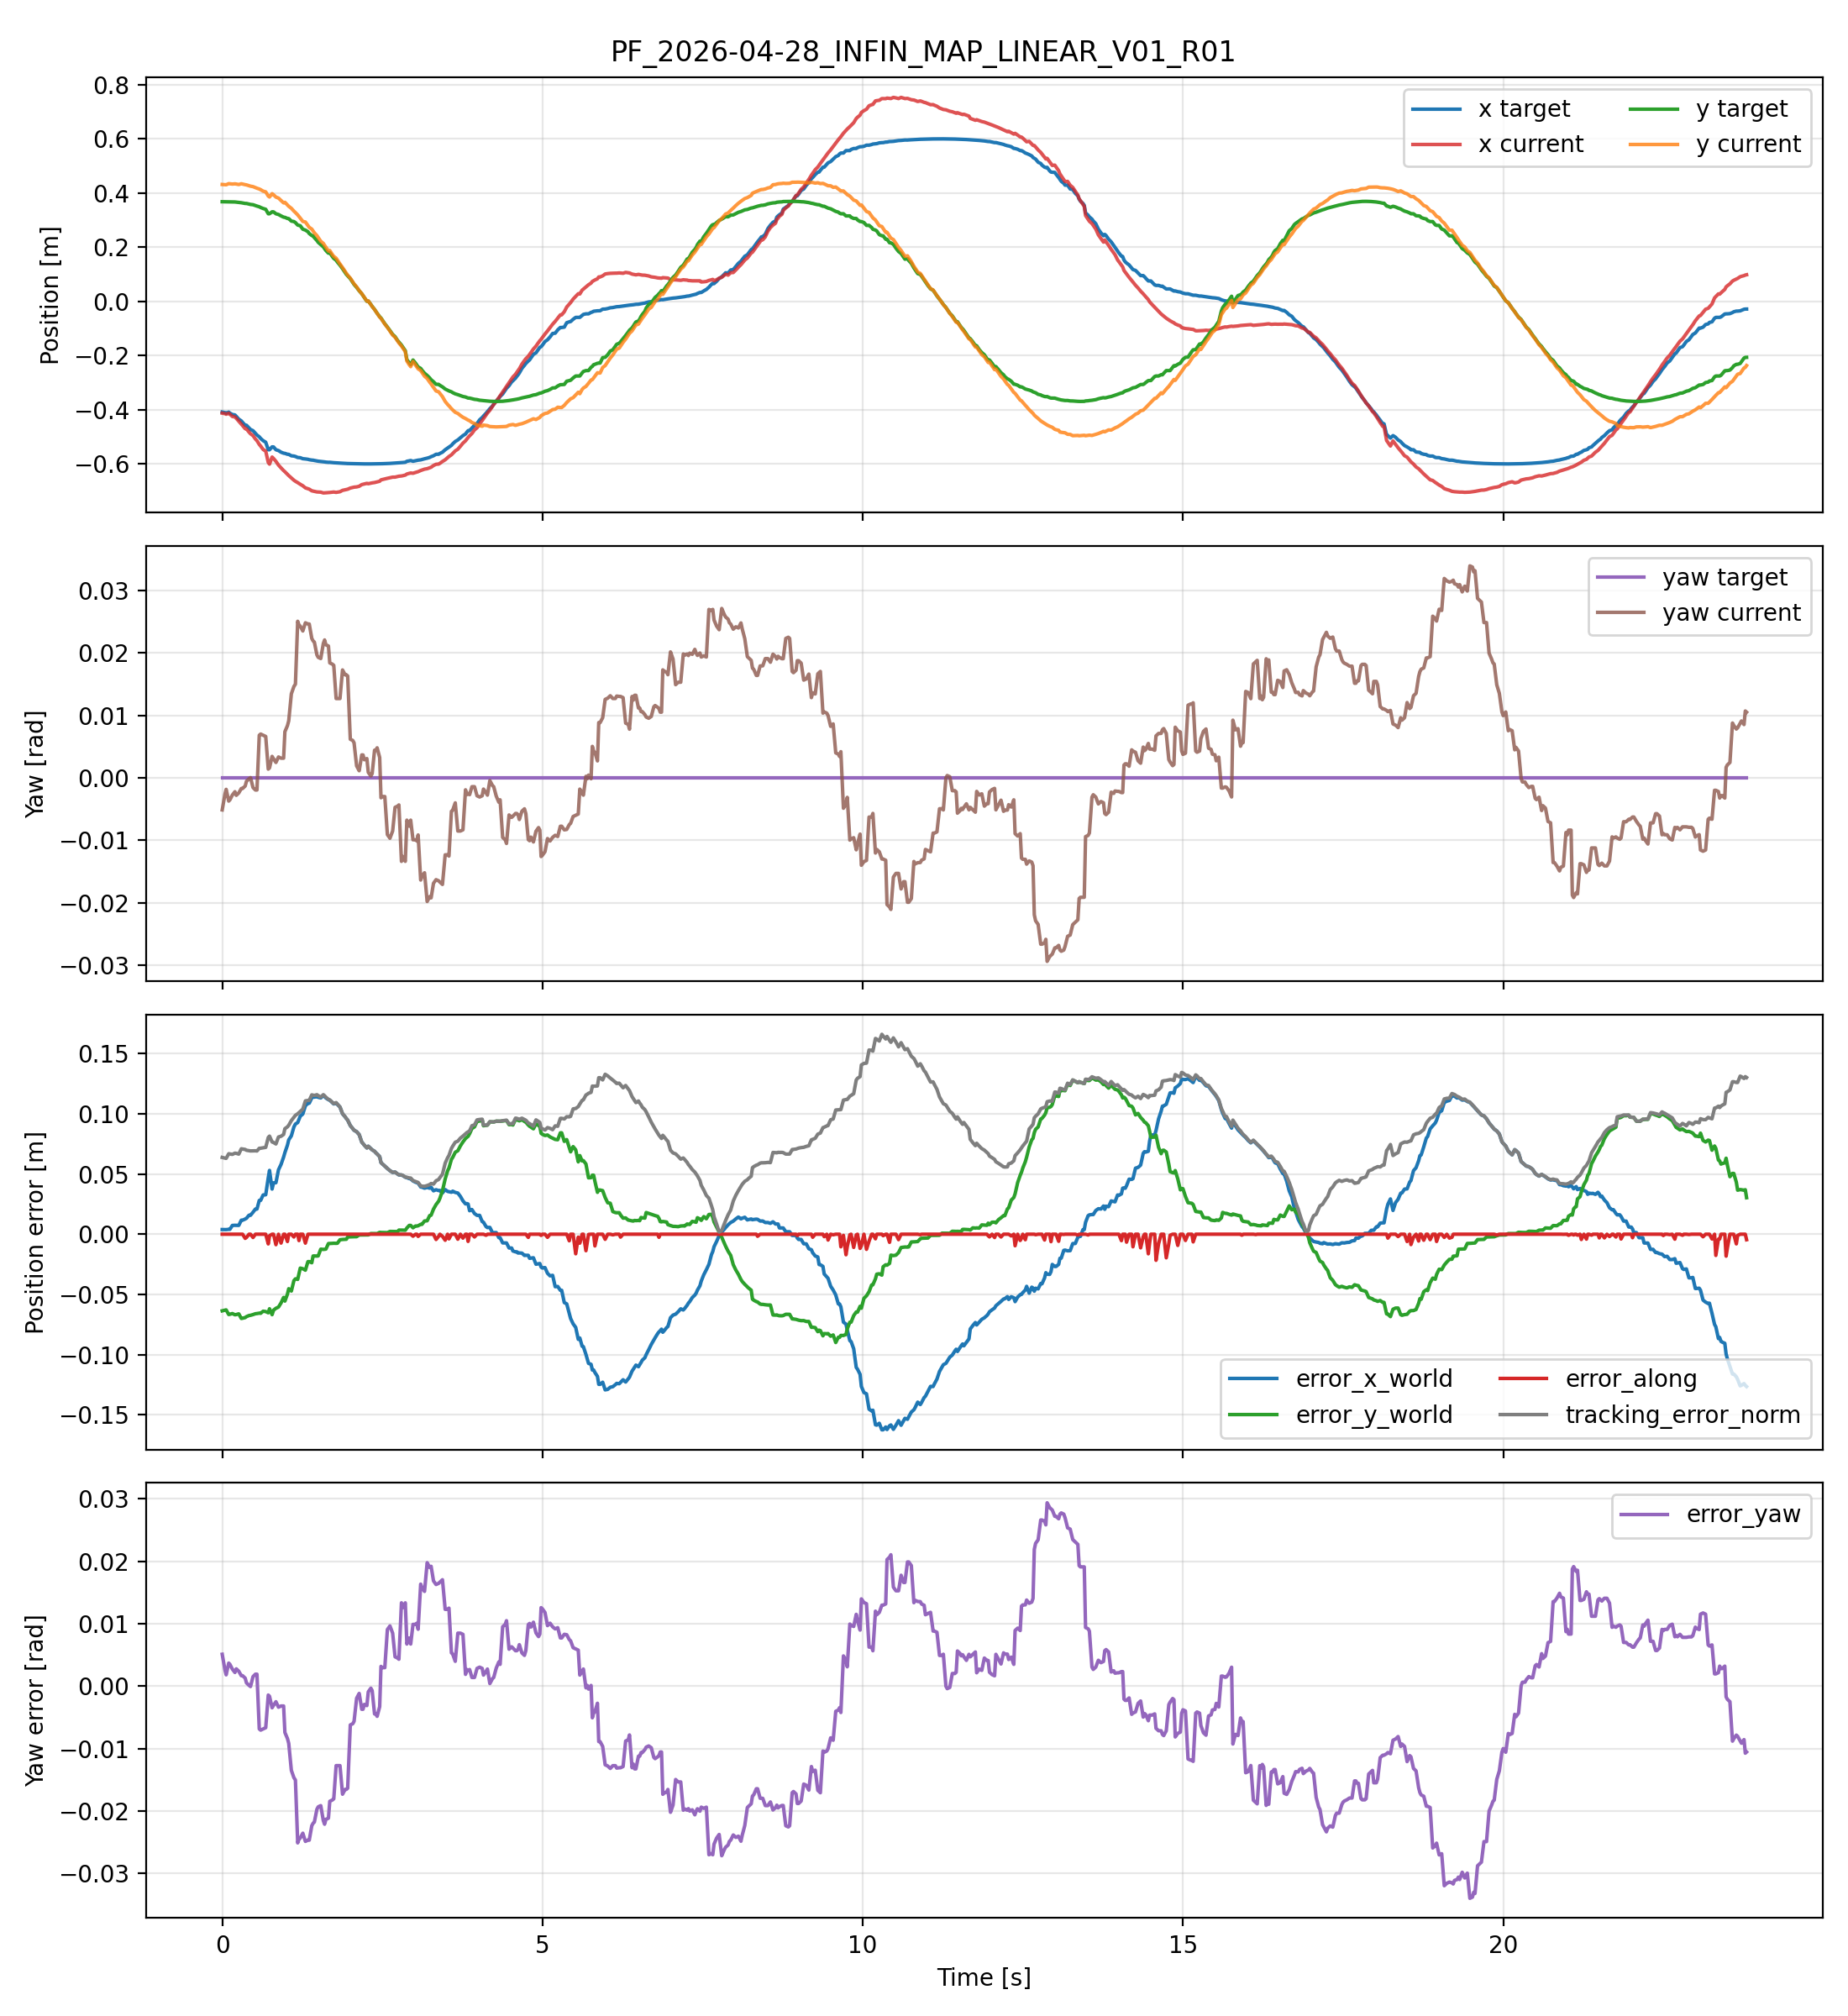
\includegraphics[width=0.7\linewidth]{IMG/controller/LIN/LIN_01_target_tracking_and_errors.png}
        \caption{LIN\_01 tracking and errors}
        \label{fig:LIN_01_tracking_and_errors}
    \end{subfigure}
    
    \vspace{0.5em}
    \caption{Experimental results for LIN\_01 scenario.} 
    \label{fig:LIN_01_general}
\end{figure}

\newpage
\begin{figure}[H]
    \centering
    \begin{subfigure}{\textwidth}
        \centering
        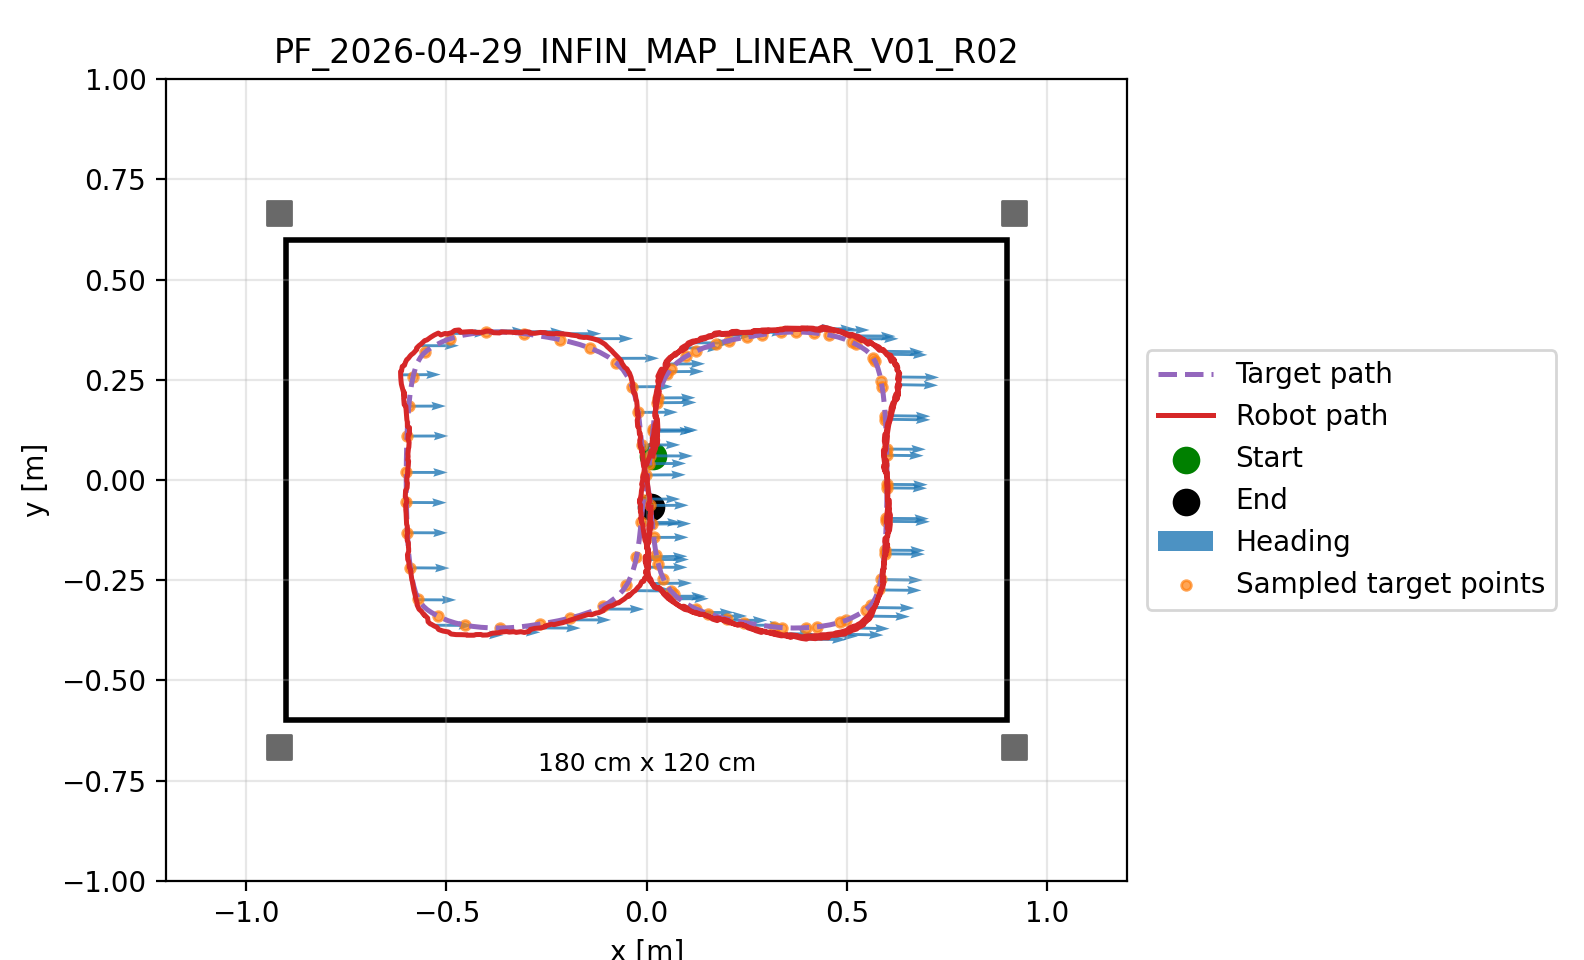
\includegraphics[width=0.7\linewidth]{IMG/controller/LIN/LIN_02_xy_map.png}
        \caption{LIN\_02 xy map}
        \label{fig:LIN_02_xy_map}
    \end{subfigure}

    \vspace{0.5em}

    \begin{subfigure}{\textwidth}
        \centering
        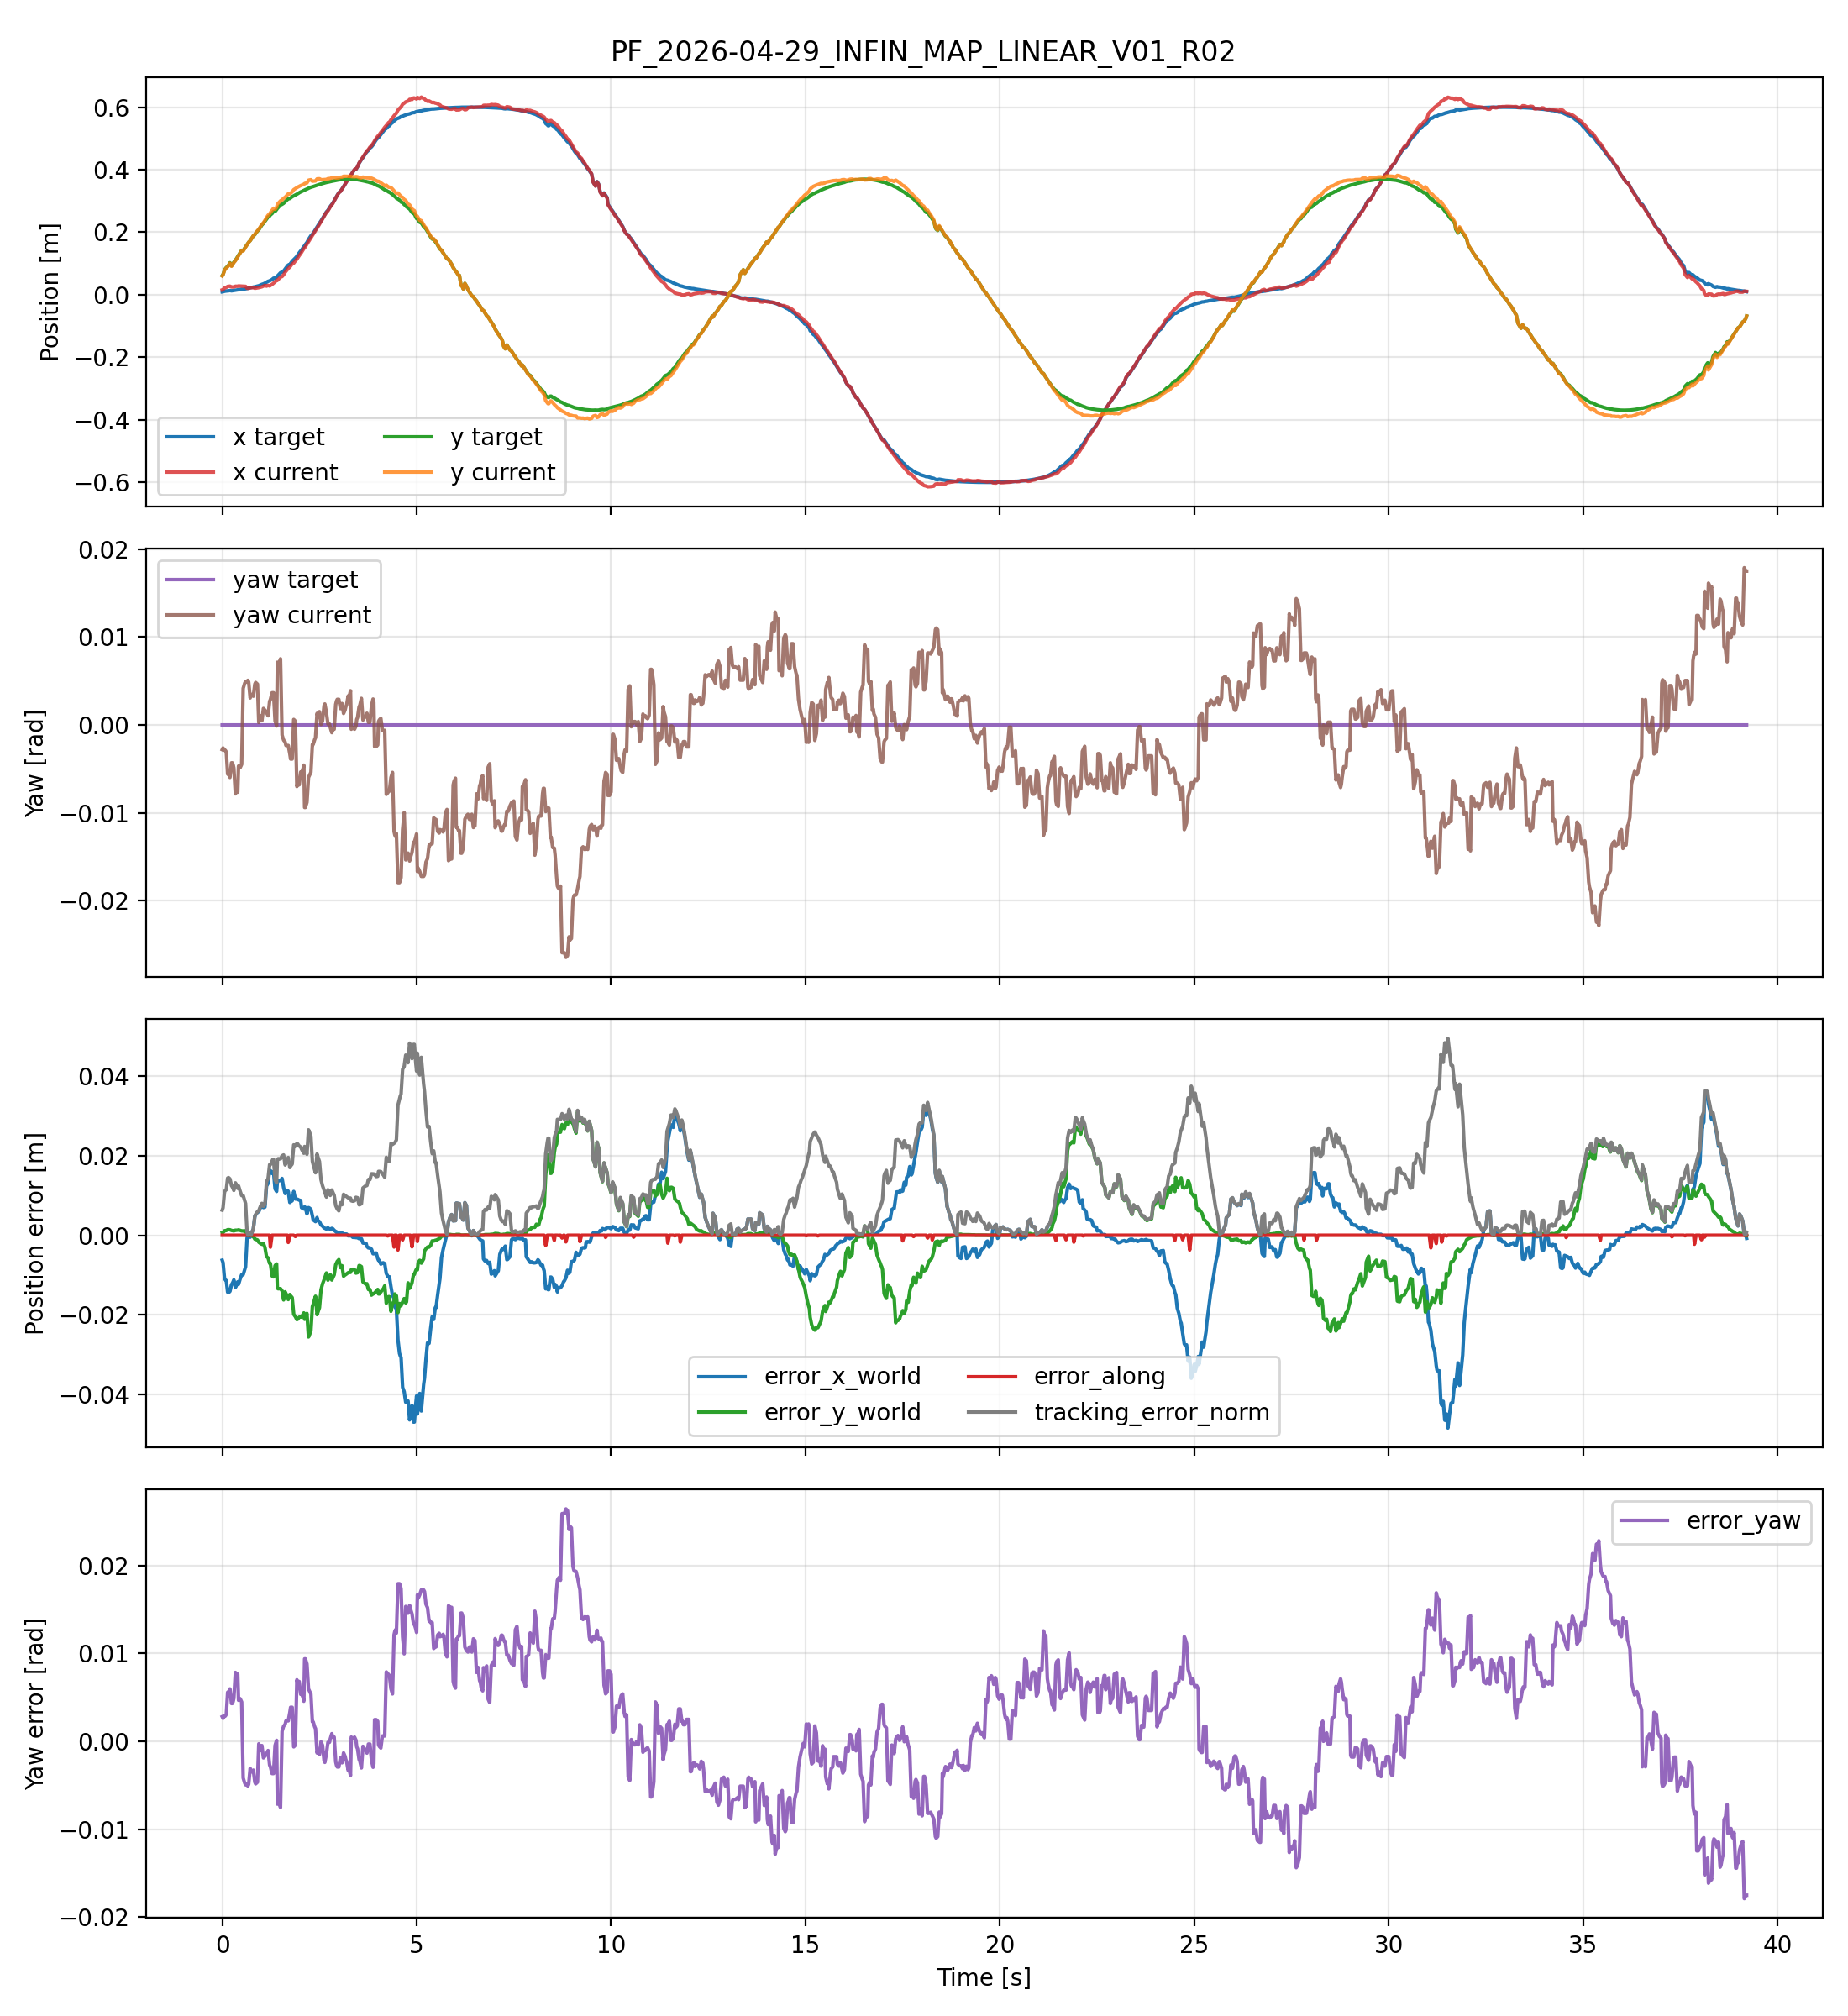
\includegraphics[width=0.7\linewidth]{IMG/controller/LIN/LIN_02_target_tracking_and_errors.png}
        \caption{LIN\_02 tracking and errors}
        \label{fig:LIN_02_tracking_and_errors}
    \end{subfigure}
    
    \vspace{0.5em}
    \caption{Experimental results for LIN\_02 scenario.} 
    \label{fig:LIN_02_general}
\end{figure}

\newpage
\begin{figure}[H]
    \centering
    \begin{subfigure}{\textwidth}
        \centering
        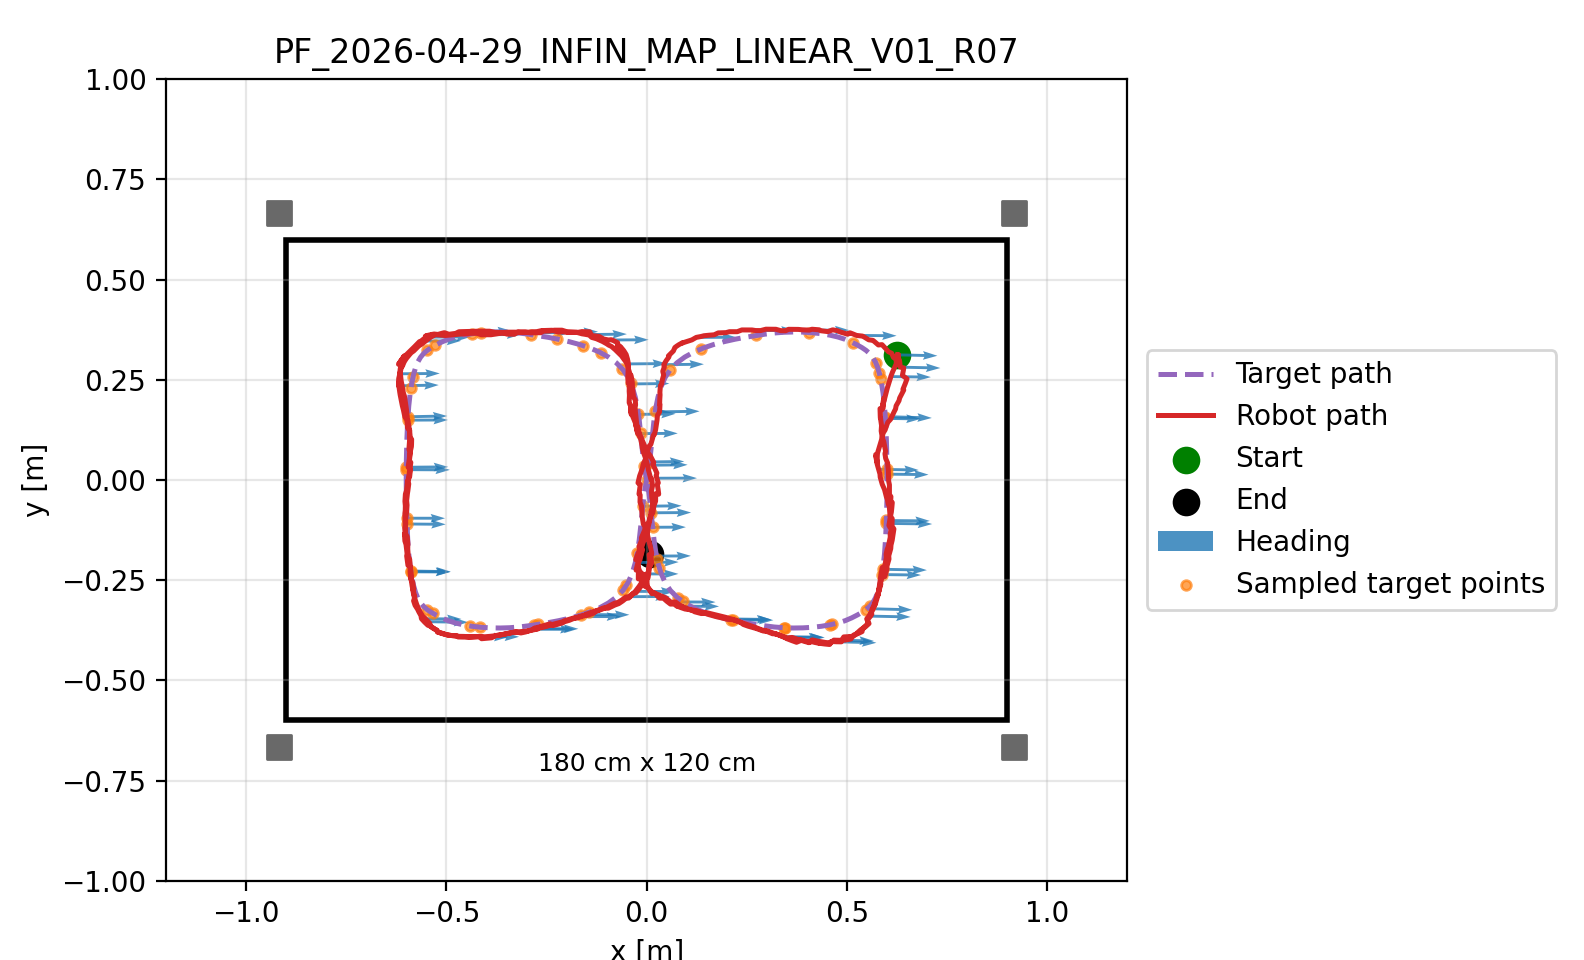
\includegraphics[width=0.7\linewidth]{IMG/controller/LIN/LIN_03_xy_map.png}
        \caption{LIN\_03 xy map}
        \label{fig:LIN_03_xy_map}
    \end{subfigure}

    \vspace{0.5em}

    \begin{subfigure}{\textwidth}
        \centering
        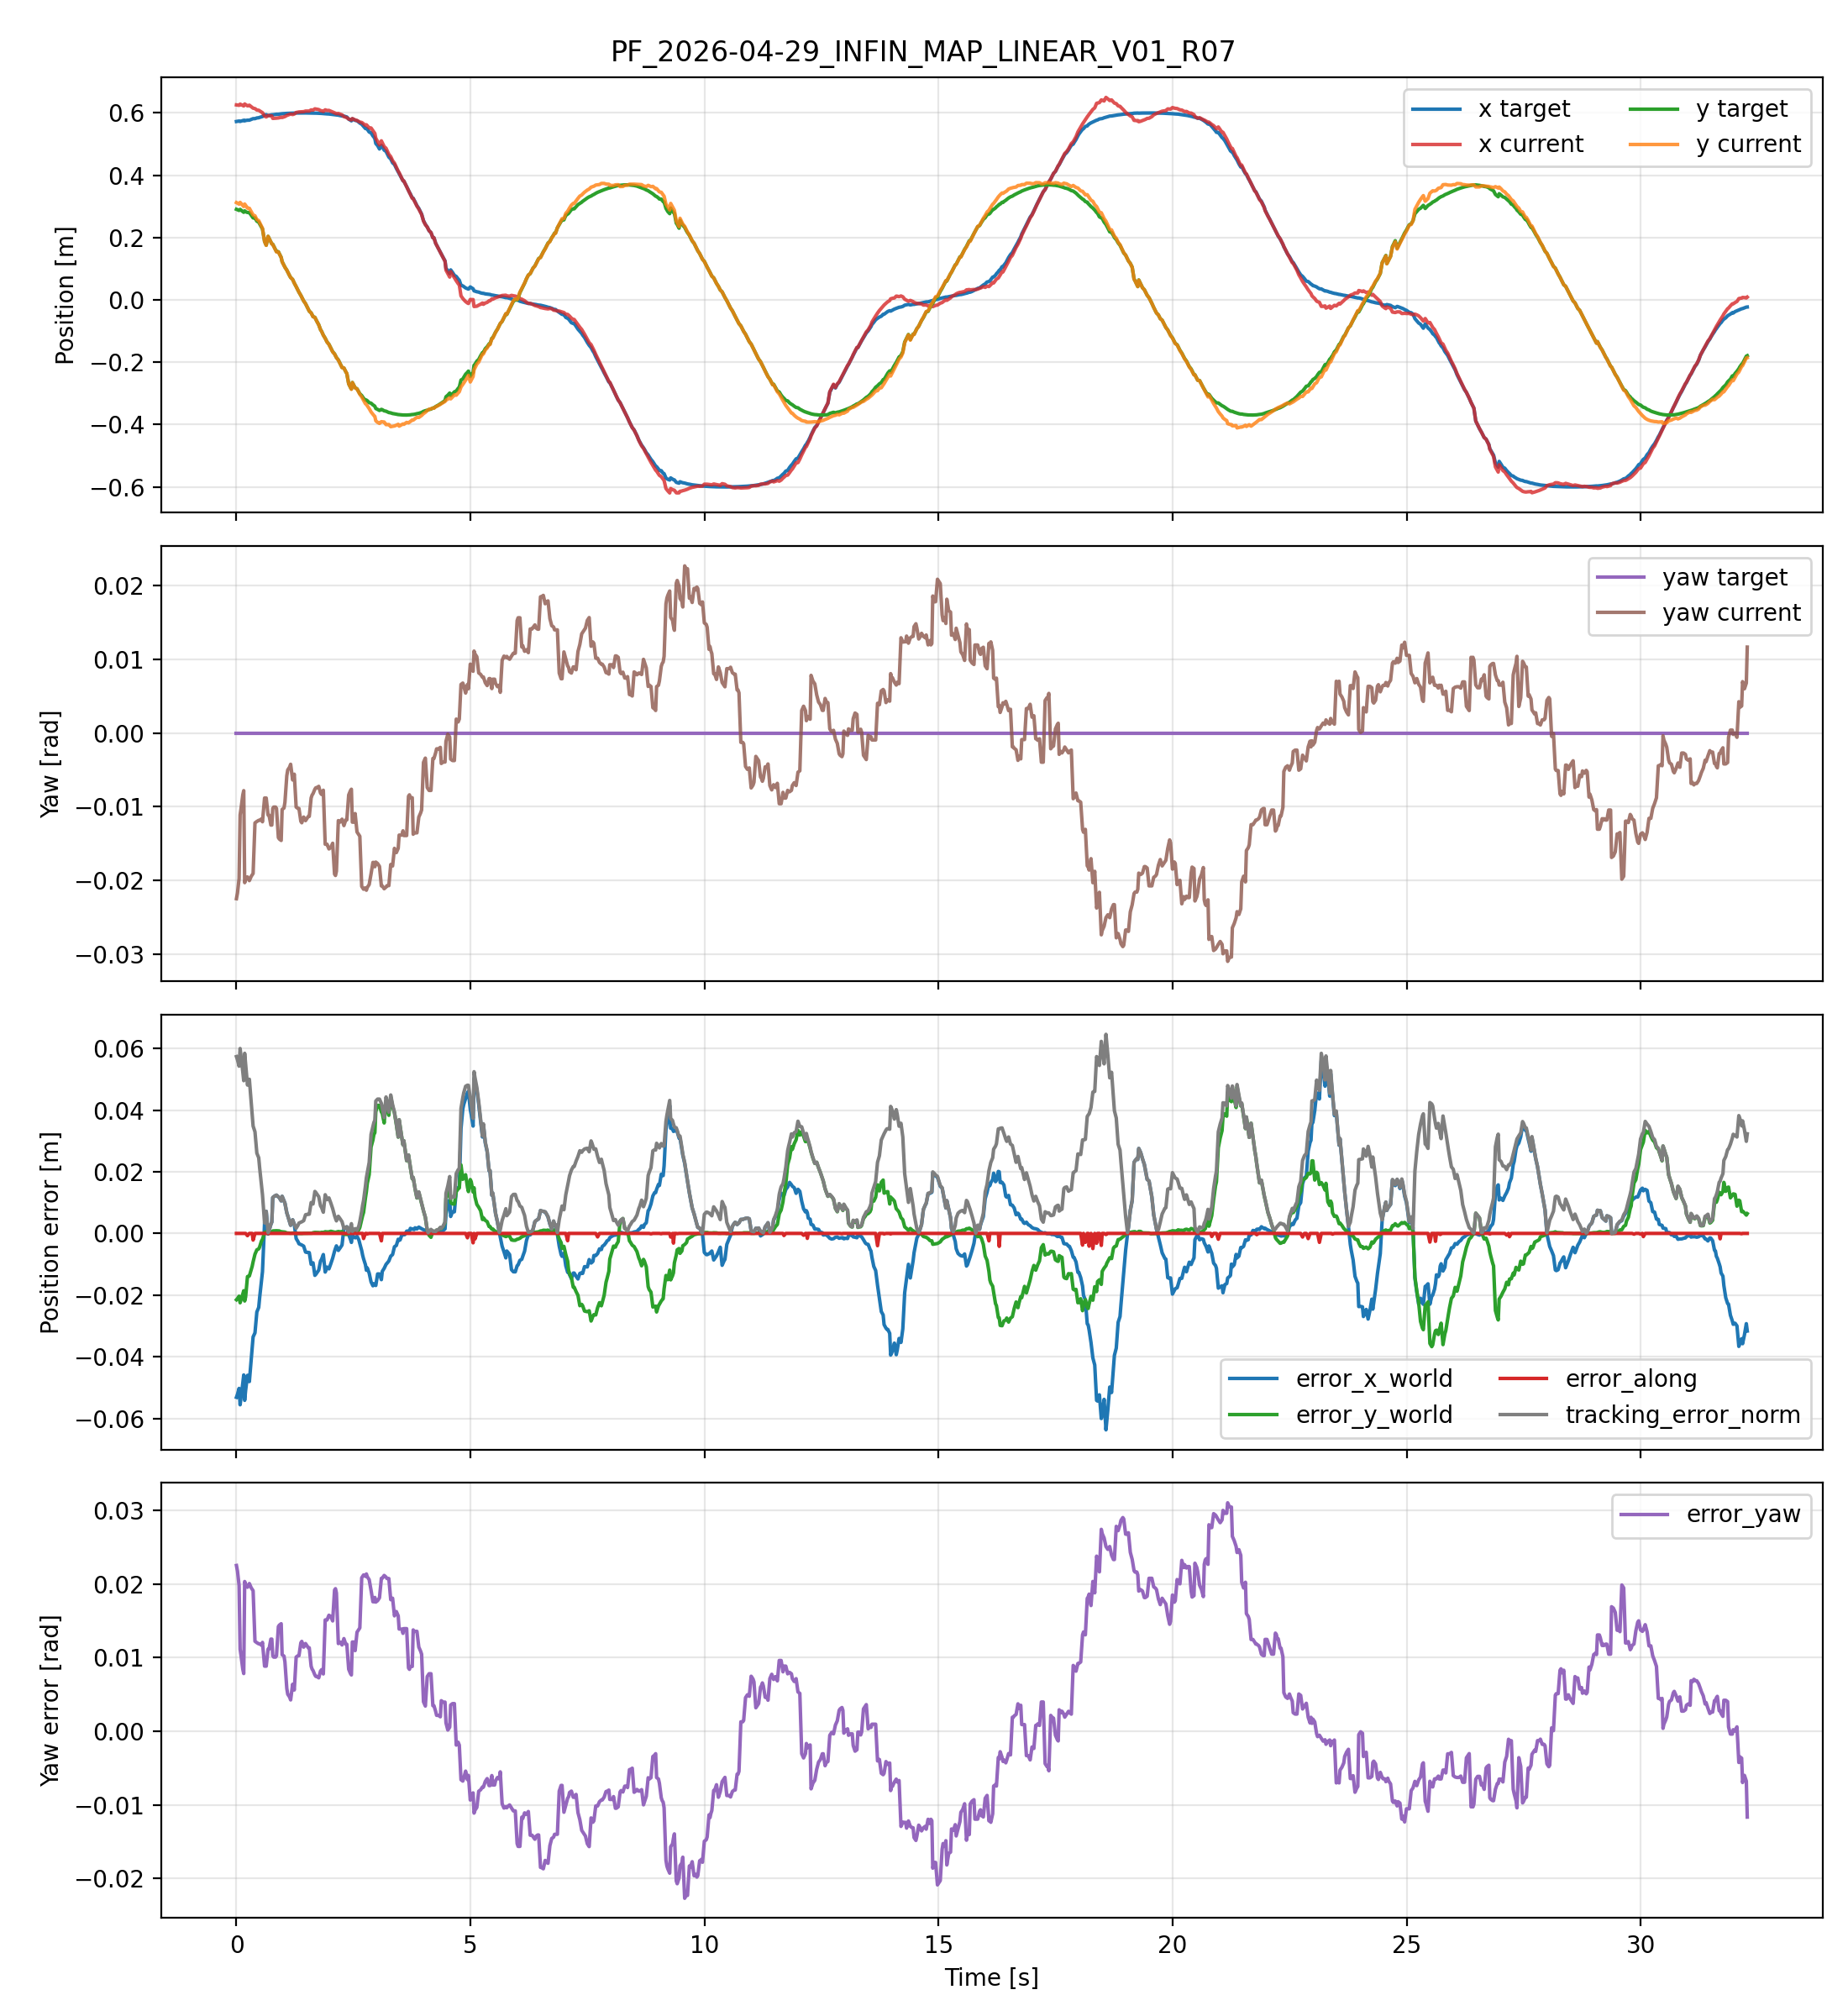
\includegraphics[width=0.7\linewidth]{IMG/controller/LIN/LIN_03_target_tracking_and_errors.png}
        \caption{LIN\_03 tracking and errors}
        \label{fig:LIN_03_tracking_and_errors}
    \end{subfigure}
    
    \vspace{0.5em}
    \caption{Experimental results for LIN\_03 scenario.} 
    \label{fig:LIN_03_general}
\end{figure}

\newpage
\begin{figure}[H]
    \centering
    \begin{subfigure}{\textwidth}
        \centering
        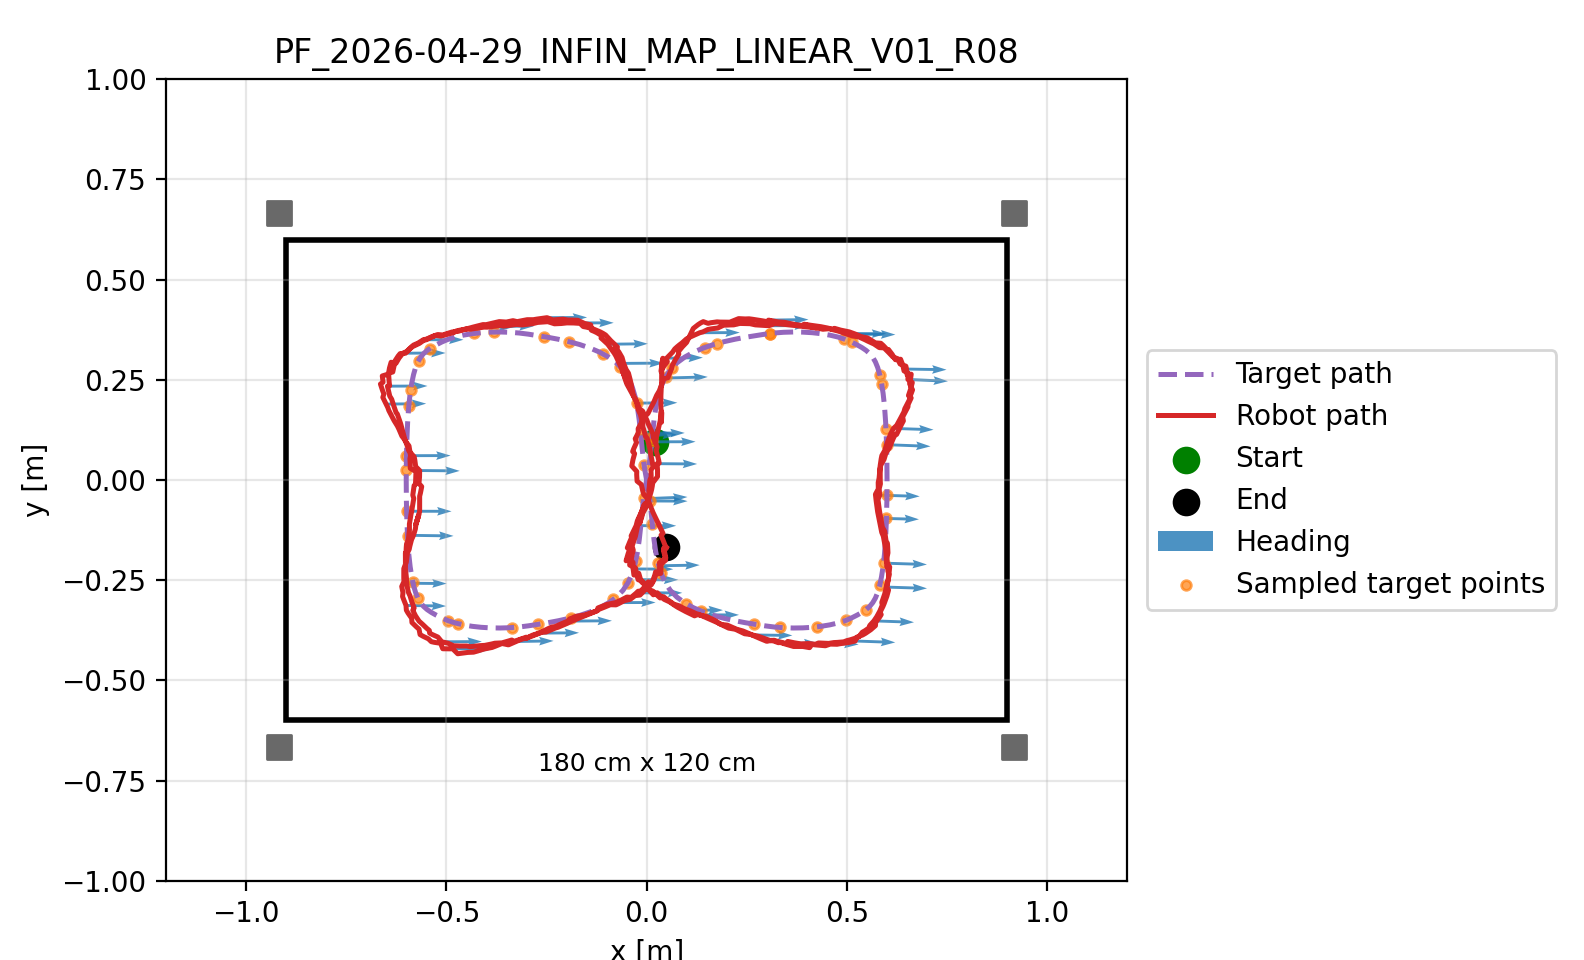
\includegraphics[width=0.7\linewidth]{IMG/controller/LIN/LIN_04_xy_map.png}
        \caption{LIN\_04 xy map}
        \label{fig:LIN_04_xy_map}
    \end{subfigure}

    \vspace{0.5em}

    \begin{subfigure}{\textwidth}
        \centering
        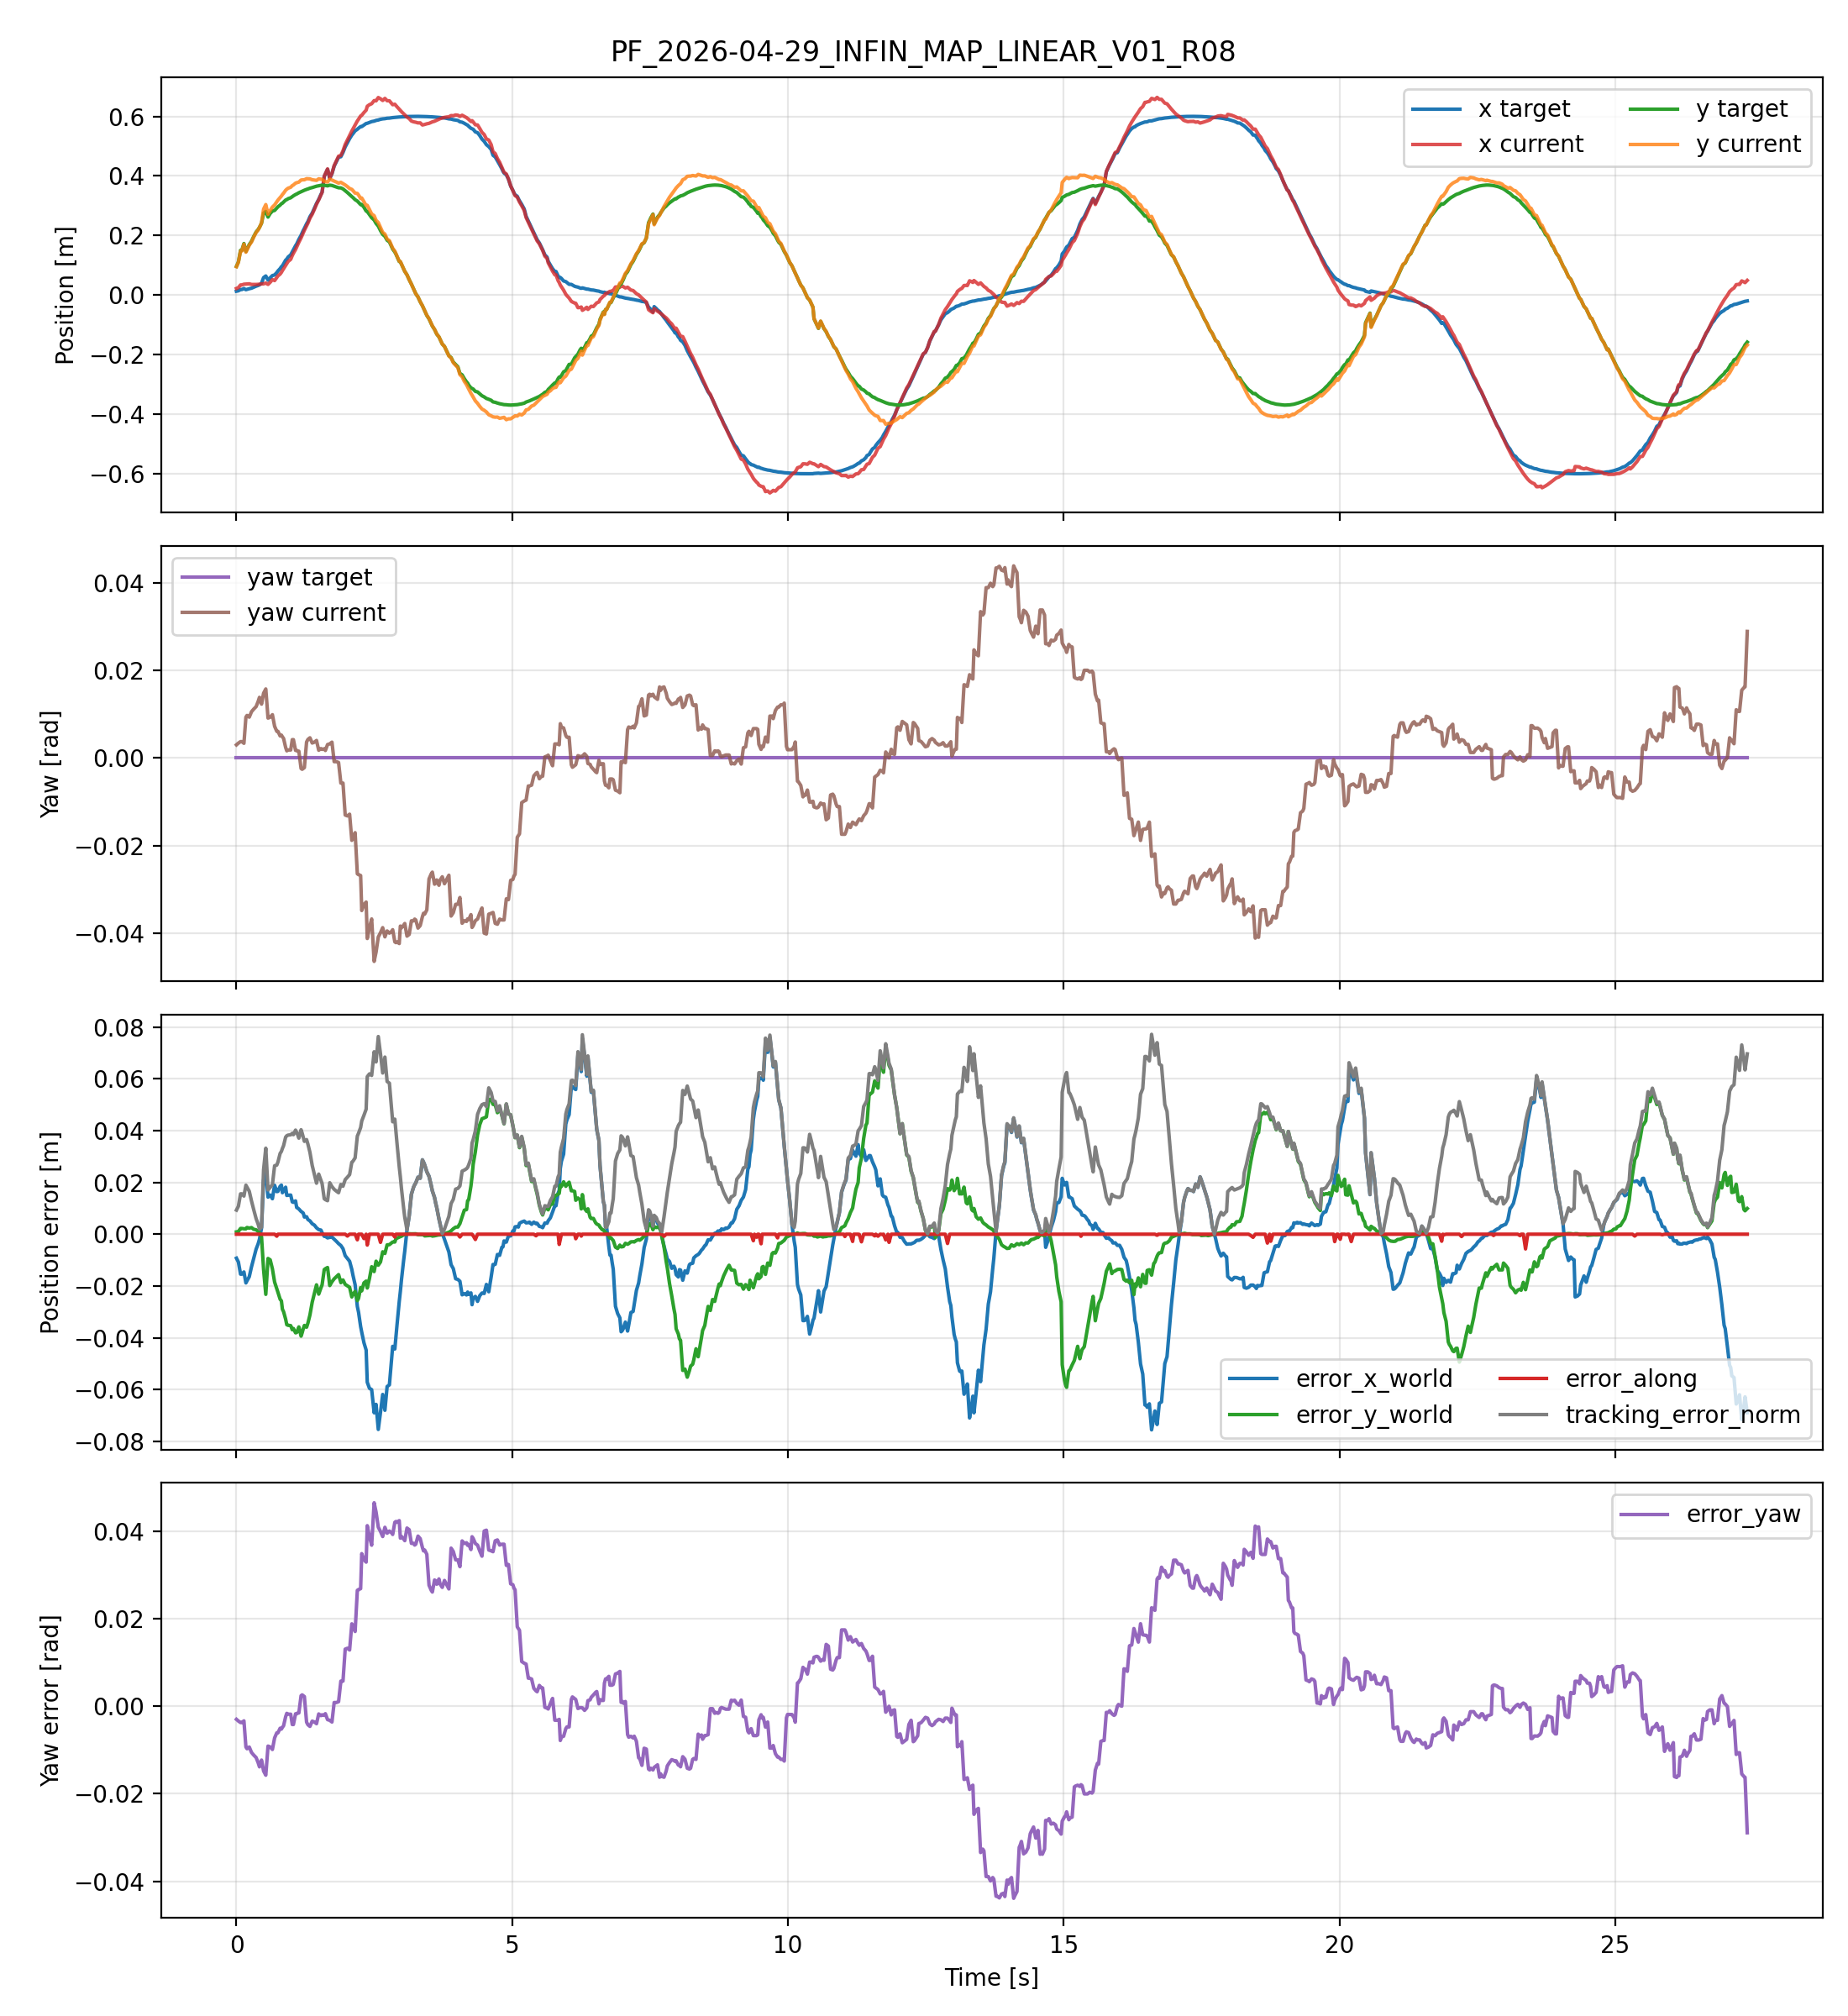
\includegraphics[width=0.7\linewidth]{IMG/controller/LIN/LIN_04_target_tracking_and_errors.png}
        \caption{LIN\_04 tracking and errors}
        \label{fig:LIN_04_tracking_and_errors}
    \end{subfigure}
    
    \vspace{0.5em}
    \caption{Experimental results for LIN\_04 scenario.} 
    \label{fig:LIN_04_general}
\end{figure}

\newpage
\begin{figure}[H]
    \centering
    \begin{subfigure}{\textwidth}
        \centering
        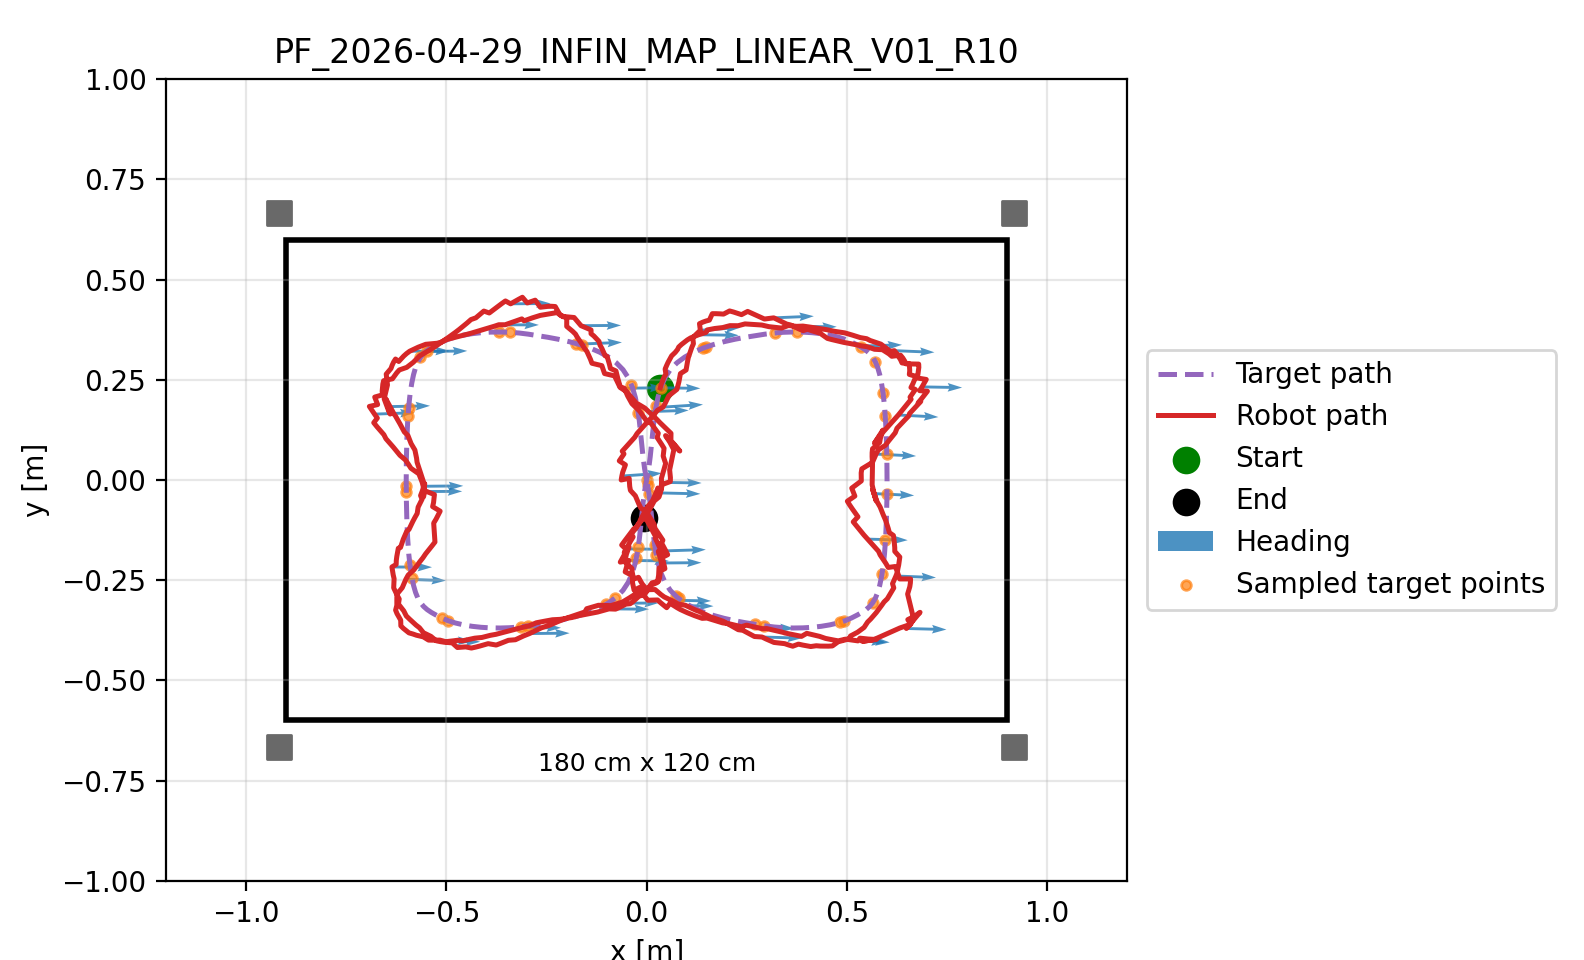
\includegraphics[width=0.7\linewidth]{IMG/controller/LIN/LIN_05_xy_map.png}
        \caption{LIN\_05 xy map}
        \label{fig:LIN_05_xy_map}
    \end{subfigure}

    \vspace{0.5em}

    \begin{subfigure}{\textwidth}
        \centering
        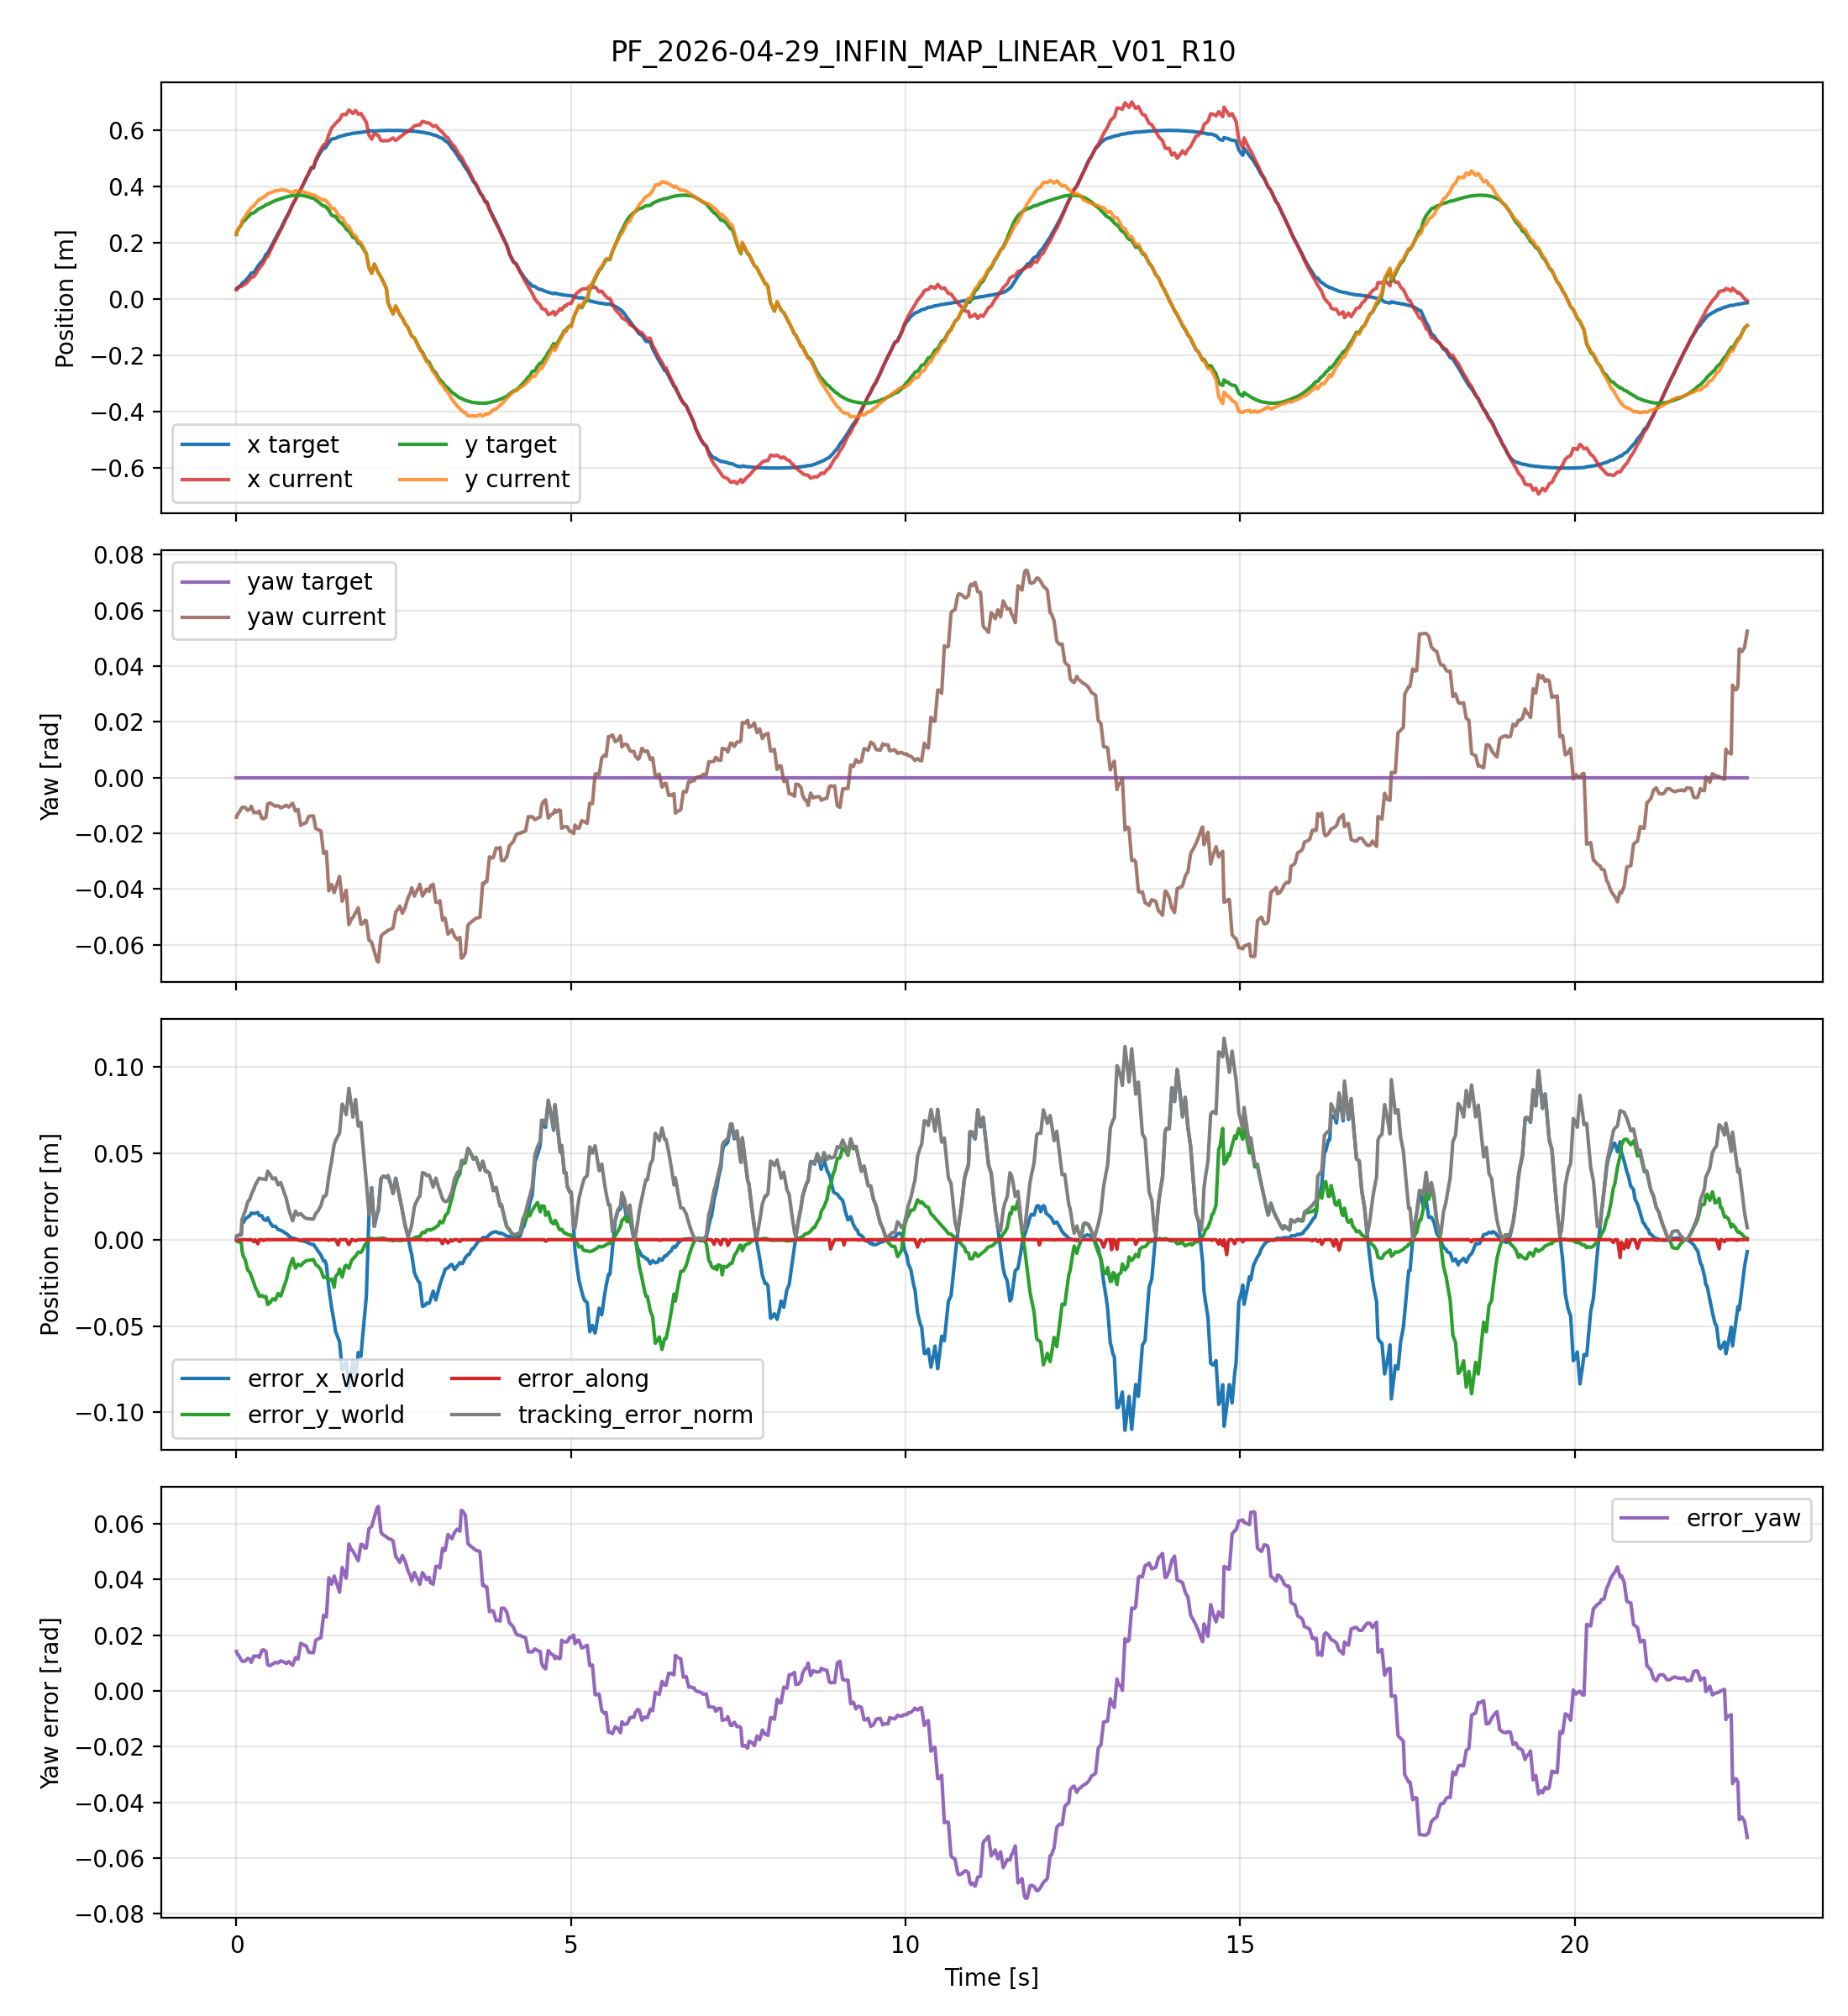
\includegraphics[width=0.7\linewidth]{IMG/controller/LIN/LIN_05_target_tracking_and_errors.png}
        \caption{LIN\_05 tracking and errors}
        \label{fig:LIN_05_tracking_and_errors}
    \end{subfigure}
    
    \vspace{0.5em}
    \caption{Experimental results for LIN\_05 scenario.} 
    \label{fig:LIN_05_general}
\end{figure}

% Section to append to Chapter 6 after the Linear Segment controller.
% Required packages: booktabs, float, subcaption.

% Section to append to Chapter 6 after the Linear Segment controller.
% Required packages: booktabs, float, subcaption.
% Code excerpts use the standard LaTeX verbatim environment.

\section{Nonlinear Model Predictive Contouring Controller}
\label{sec:nonlinear_mpcc_controller}

This section describes the predictive controller used in the experimental.  The objective of the controller is not only to
reduce the instantaneous Cartesian error with respect to a moving point, but to
choose a velocity command by considering the future evolution of the robot over a
short horizon.  This is the main difference with the previous geometric
controllers: the command is selected by balancing path accuracy, path
progression, command effort and command smoothness in the same optimization
problem.

The formulation is inspired by MPC trajectory-tracking approaches for
omnidirectional mobile robots.  In those approaches a model of the robot is used
to predict the future motion, and an optimal control problem is solved at each
control period.  Smooth parametric references, such as B-Spline trajectories, are
particularly suitable for MPC because the reference can be evaluated at any point
of the prediction horizon and the local path geometry can be used inside the
cost function.  In this work the reference is treated as a geometric path rather
than as a purely time-indexed trajectory.  The progression along the path is
represented by the curvilinear coordinate \(\gamma\), so the controller can
separate lateral path error from advancement along the curve.

The controller follows the same cascade architecture used in the rest of the
ROS2 stack.  The high-level node receives the estimated pose in the
\texttt{map} frame, evaluates the reference path, computes a planar velocity
command and publishes a \texttt{geometry\_msgs/Twist} message on
\texttt{cmd\_vel}.  The lower ROS2 driver and the ESP32 firmware then convert
this velocity reference into wheel commands and motor voltages.

\subsection{Geometric Path Representation}

The reference path is represented by a sequence of points loaded from a CSV file.
The implementation stores the cumulative distance along the polyline, which is
used as the path coordinate \(\gamma\).  Given \(\gamma\), the function
\texttt{sampleAt} finds the corresponding segment, interpolates the reference
position and computes the local tangent:

\begin{verbatim}
PathSample sampleAt(double gamma) const
{
  ...
  sample.x = a.x + ratio * (b.x - a.x);
  sample.y = a.y + ratio * (b.y - a.y);
  sample.tangent_x = (b.x - a.x) / segment_length;
  sample.tangent_y = (b.y - a.y) / segment_length;
  ...
}
\end{verbatim}

The tangent vector is therefore
\begin{equation}
    \mathbf{t}(\gamma)=
    \begin{bmatrix}
        t_x(\gamma) & t_y(\gamma)
    \end{bmatrix}^{T},
\end{equation}
while the normal vector is obtained as
\begin{equation}
    \mathbf{n}(\gamma)=
    \begin{bmatrix}
        -t_y(\gamma) & t_x(\gamma)
    \end{bmatrix}^{T}.
\end{equation}
This same geometric representation is used by the Linear Segment controller and
is the natural basis for the MPCC formulation, because contouring and lag errors
are defined with respect to the tangent and normal directions of the path.

\subsection{Predictive Model}

The predicted state is defined as
\begin{equation}
    \mathbf{x}_k =
    \begin{bmatrix}
        x_k & y_k & \psi_k & \gamma_k
    \end{bmatrix}^{T},
\end{equation}
where \((x_k,y_k,\psi_k)\) is the predicted robot pose and \(\gamma_k\) is the
predicted curvilinear coordinate along the path.  The control vector is
\begin{equation}
    \mathbf{u}_k =
    \begin{bmatrix}
        v_{x,k} & v_{y,k} & \omega_k & \dot{\gamma}_k
    \end{bmatrix}^{T}.
\end{equation}
The first three variables are the body-frame velocity command sent to the robot,
whereas \(\dot{\gamma}_k\) controls the virtual advancement of the reference
point along the path.

The prediction model is the discrete-time kinematic model of a holonomic mobile
robot:
\begin{equation}
\begin{aligned}
    x_{k+1} &= x_k + \Delta t
    \left(\cos\psi_k\,v_{x,k}-\sin\psi_k\,v_{y,k}\right), \\
    y_{k+1} &= y_k + \Delta t
    \left(\sin\psi_k\,v_{x,k}+\cos\psi_k\,v_{y,k}\right), \\
    \psi_{k+1} &= \mathrm{wrapToPi}(\psi_k + \Delta t\,\omega_k), \\
    \gamma_{k+1} &= \gamma_k + \Delta t\,\dot{\gamma}_k .
\end{aligned}
\end{equation}
This model is intentionally simple: it assumes that the omnidirectional platform
can track the commanded planar velocity directly.  Therefore, wheel dynamics,
slip, actuator dead zones and low-level loop delays are not part of the
prediction model.  In the experimental tests the prediction step is
\(\Delta t=0.08~\mathrm{s}\).  The horizon is usually \(N=12\), corresponding to
a prediction window of approximately \(0.96~\mathrm{s}\), while the final test
uses \(N=14\), corresponding to approximately \(1.12~\mathrm{s}\).

\subsection{Contouring and Lag Errors}

At each predicted step the path is sampled at \(\gamma_k\).  Let
\(\mathbf{p}_k=[x_k\;y_k]^T\) be the predicted robot position and
\(\mathbf{p}_r(\gamma_k)\) the sampled reference point.  The position error is
projected onto the tangent and normal directions:
\begin{equation}
    e_{l,k} =
    \left(\mathbf{p}_k-\mathbf{p}_r(\gamma_k)\right)^T
    \mathbf{t}(\gamma_k),
    \qquad
    e_{c,k} =
    \left(\mathbf{p}_k-\mathbf{p}_r(\gamma_k)\right)^T
    \mathbf{n}(\gamma_k).
\end{equation}
The lag error \(e_l\) measures whether the predicted robot position is ahead of
or behind the virtual reference point along the path.  The contouring error
\(e_c\) measures the lateral deviation from the path and is the most important
quantity for geometric path following.  The heading error is
\begin{equation}
    e_{\psi,k}=\mathrm{wrapToPi}(\psi_r(\gamma_k)-\psi_k).
\end{equation}

The same decomposition can be seen in the available path-following code used for
the Linear Segment controller.  The controller computes the tangent, builds the
normal vector, and projects the Cartesian error onto both directions:

\begin{verbatim}
const double normal_x = -command.target.tangent_y;
const double normal_y = command.target.tangent_x;
const double error_along =
  dx_world * command.target.tangent_x + dy_world * command.target.tangent_y;
const double error_lateral = dx_world * normal_x + dy_world * normal_y;
\end{verbatim}

For the MPCC, these same geometric quantities are evaluated not only at the
current pose, but at every predicted state along the horizon.

\subsection{Cost Function}

The stage cost minimized along the horizon is composed of tracking, progress,
effort and smoothness terms:
\begin{equation}
\begin{aligned}
    J_k =&
    q_c e_{c,k}^{2}
    + q_l e_{l,k}^{2}
    + q_{\psi} e_{\psi,k}^{2}
    - q_p \dot{\gamma}_k \\
    &+ r_{v_x} v_{x,k}^{2}
    + r_{v_y} v_{y,k}^{2}
    + r_{\omega} \omega_k^{2}
    + r_{\dot{\gamma}} \dot{\gamma}_k^{2} \\
    &+ r_{\Delta v_x}\Delta v_{x,k}^{2}
    + r_{\Delta v_y}\Delta v_{y,k}^{2}
    + r_{\Delta\omega}\Delta\omega_k^{2}
    + r_{\Delta\dot{\gamma}}\Delta\dot{\gamma}_k^{2}.
\end{aligned}
\end{equation}
The terms \(q_c\), \(q_l\) and \(q_{\psi}\) penalize geometric tracking errors.
The negative term \(-q_p\dot{\gamma}_k\) rewards advancement along the path.  The
\(r\) terms penalize large velocity commands, while the \(r_\Delta\) terms
penalize command increments.  Penalizing increments is important in practice
because it reduces abrupt changes in \texttt{cmd\_vel} without forcing the
absolute velocity to be unnecessarily small.  A terminal cost is also added to
the last predicted contouring and lag errors, so the final state of the rollout
is encouraged to remain close to the path.

\subsection{Implementation Structure}

The ROS2 path-following node is organized around a common control pipeline:
receive the pose, compute a \texttt{ControlCommand}, and publish the final
\texttt{Twist}.  In the public repository version, the dispatcher selects between
\texttt{linear\_segment} and \texttt{moving\_reference\_p}:

\begin{verbatim}
void runFollow(const rclcpp::Time & stamp, double dt)
{
  ControlCommand command = controller_mode_ == "linear_segment" ?
    computeLinearSegmentCommand() :
    computeMovingReferenceCommand(dt);
  publishCommand(stamp, dt, command);
}
\end{verbatim}

The MPCC controller follows the same interface: it must return a
\texttt{ControlCommand} containing the selected body-frame velocities and the
predicted path advancement.  Conceptually, the dispatcher becomes:

\begin{verbatim}
if (controller_mode_ == "linear_segment") {
  command = computeLinearSegmentCommand();
} else if (controller_mode_ == "moving_reference_p") {
  command = computeMovingReferenceCommand(dt);
} else if (controller_mode_ == "nonlinear_mpcc") {
  command = computeNonlinearMpccCommand(dt);
}
\end{verbatim}

The sampled MPCC implementation can be summarized by the following pseudo-code:

\begin{verbatim}
best_cost = +infinity
best_command = previous_command

for vx in sampled_vx:
  for vy in sampled_vy:
    for omega in sampled_omega:
      for gamma_dot in sampled_gamma_dot:
        x_pred = current_x
        y_pred = current_y
        psi_pred = current_yaw
        gamma_pred = current_gamma
        cost = 0

        for k = 0 ... N-1:
          sample = sampleAt(gamma_pred)
          t = sample.tangent
          n = [-t.y, t.x]

          e_l = dot([x_pred,y_pred] - sample.position, t)
          e_c = dot([x_pred,y_pred] - sample.position, n)
          e_psi = wrapToPi(sample.yaw - psi_pred)

          cost += stageCost(e_c, e_l, e_psi,
                            vx, vy, omega, gamma_dot,
                            previous_command)

          x_pred += dt * (cos(psi_pred)*vx - sin(psi_pred)*vy)
          y_pred += dt * (sin(psi_pred)*vx + cos(psi_pred)*vy)
          psi_pred = wrapToPi(psi_pred + dt * omega)
          gamma_pred += dt * gamma_dot

        cost += terminalCost(e_c, e_l)

        if cost < best_cost:
          best_cost = cost
          best_command = [vx, vy, omega, gamma_dot]
\end{verbatim}

After the best candidate is selected, it is published through the same output
stage used by the other controllers.  The current node adds feedforward and
feedback terms, saturates the velocities and publishes \texttt{cmd\_vel}:

\begin{verbatim}
cmd.linear.x = clamp(cmd_vx_raw, -max_linear_x_, max_linear_x_);
cmd.linear.y = clamp(cmd_vy_raw, -max_linear_y_, max_linear_y_);
cmd.angular.z = clamp(cmd_w_raw, -max_angular_z_, max_angular_z_);
pub_cmd_vel_->publish(cmd);
\end{verbatim}

This implementation choice avoids the need for an external nonlinear optimizer
and is deterministic, but the result depends on the sampling resolution.  A
coarse grid is computationally cheap but may produce quantized commands, whereas
a dense grid improves the approximation at the cost of a higher computation
time.

\subsection{Limitations and Possible Improvements}

The main limitations of this first predictive formulation are:
\begin{itemize}
    \item the prediction model neglects wheel dynamics, actuator delay, wheel
    slip, friction and the transient response of the low-level velocity loop;
    \item the command is selected on a finite grid, so the solution is only an
    approximation of the continuous optimum;
    \item the same candidate command is kept constant during the whole rollout,
    which reduces computation time but limits the richness of the predicted
    control sequence;
    \item the controller depends directly on the pose estimate, so localization
    drift appears as contouring and lag error;
    \item obstacle constraints are not included, therefore the controller is a
    path-following controller and not a complete local planner.
\end{itemize}

Future work should focus on a continuous nonlinear solver, optimization of a full
command sequence instead of a constant command, curvature-dependent velocity
limits, adaptive progress weights, explicit actuator-delay compensation and
uncertainty-aware localization handling.  The current implementation is
therefore best interpreted as an experimental predictive baseline: it shows how
tracking, progress and smoothness can be traded off explicitly, but it still
requires further tuning before it can be considered superior to a simpler and
well-tuned geometric controller in all metrics.

\subsection{Test Parameters and Results}

\noindent
\textbf{Test legend:}
\begin{itemize}
    \item \textbf{MPC-01}: \texttt{PF\_2026-05-11\_INFIN\_MAP\_MPCC\_V01\_R01};
    \item \textbf{MPC-02}: \texttt{PF\_2026-05-11\_INFIN\_MAP\_MPCC\_V01\_R02};
    \item \textbf{MPC-03}: \texttt{PF\_2026-05-11\_INFIN\_MAP\_MPCC\_V01\_R03};
    \item \textbf{MPC-04}: \texttt{PF\_2026-05-11\_INFIN\_MAP\_MPCC\_V01\_R04};
    \item \textbf{MPC-05}: \texttt{PF\_2026-05-11\_INFIN\_MAP\_MPCC\_V01\_R05};
    \item \textbf{MPC-06}: \texttt{PF\_2026-05-11\_INFIN\_MAP\_MPCC\_V01\_R06}.
\end{itemize}

The following parameters are common to all tests: path \texttt{INFIN}, reference frame
\texttt{MAP}, controller mode \texttt{nonlinear\_mpcc}, fixed heading mode.

\begin{table}[H]
\centering
\caption{Main characteristic parameters of the selected MPCC tests.}
\label{tab:mpcc_characteristic_parameters}
\scriptsize
\setlength{\tabcolsep}{3pt}
\renewcommand{\arraystretch}{1.05}
\begin{tabular}{lcccccc}
\toprule
\textbf{Parameter} &
\textbf{MPC-01} &
\textbf{MPC-02} &
\textbf{MPC-03} &
\textbf{MPC-04} &
\textbf{MPC-05} &
\textbf{MPC-06} \\
\midrule
Main configuration 
& Baseline 
& Slow/stable 
& Aggressive 
& Very aggressive 
& Aggressive curves 
& Extreme \\
\midrule
\(v_{x,\max}\) [m/s]          
& 0.25 & 0.18 & 0.35 & 0.50 & 0.60 & 0.70 \\
\(v_{y,\max}\) [m/s]          
& 0.25 & 0.18 & 0.35 & 0.50 & 0.60 & 0.70 \\
\(\omega_{\max}\) [rad/s]     
& 0.45 & 0.35 & 0.60 & 0.60 & 0.60 & 0.80 \\
\(\dot{\gamma}_{\max}\) [m/s] 
& 0.30 & 0.20 & 0.40 & 0.40 & 0.40 & 0.70 \\
\midrule
\(a_{x,\max}\) [m/s\(^2\)]    
& 0.60 & 0.40 & 0.90 & 0.90 & 0.90 & 1.80 \\
\(a_{y,\max}\) [m/s\(^2\)]    
& 0.60 & 0.40 & 0.90 & 0.90 & 0.90 & 1.80 \\
\(\dot{\omega}_{\max}\) [rad/s\(^2\)] 
& 1.20 & 0.80 & 1.60 & 1.60 & 1.60 & 2.50 \\
\(\ddot{\gamma}_{\max}\) [m/s\(^2\)] 
& 0.80 & 0.50 & 1.20 & 1.20 & 1.20 & 2.50 \\
\midrule
\(q_p\)                       
& 0.40 & 0.25 & 0.60 & 0.60 & 0.90 & 1.60 \\
\(q_c\)                       
& 20 & 20 & 20 & 20 & 20 & 18 \\
\(q_l\)                       
& 2 & 2 & 2 & 2 & 2 & 1 \\
\(q_{\psi}\)                  
& 1.0 & 1.0 & 1.0 & 1.0 & 1.0 & 0.6 \\
\midrule
\(r_{v_x}, r_{v_y}\)          
& 0.15 & 0.15 & 0.15 & 0.15 & 0.15 & 0.07 \\
\(r_{\omega}\)                
& 0.10 & 0.10 & 0.10 & 0.10 & 0.10 & 0.05 \\
\(r_{\dot{\gamma}}\)          
& 0.05 & 0.05 & 0.05 & 0.05 & 0.05 & 0.02 \\
\(r_{\Delta v_x}, r_{\Delta v_y}\) 
& 0.50 & 0.50 & 0.50 & 0.50 & 0.70 & 0.25 \\
\(r_{\Delta \omega}\)         
& 0.20 & 0.20 & 0.20 & 0.20 & 0.20 & 0.10 \\
\(r_{\Delta \dot{\gamma}}\)   
& 0.10 & 0.10 & 0.10 & 0.10 & 0.10 & 0.30 \\
\midrule
\(N\)                         
& 12 & 12 & 12 & 12 & 12 & 14 \\
\(\dot{\gamma}\) samples      
& 5 & 5 & 5 & 5 & 5 & 7 \\
\bottomrule
\end{tabular}
\end{table}

\begin{table}[H]
\centering
\caption{Compact notation used for vector parameters.}
\label{tab:mpcc_vector_parameters}
\scriptsize
\setlength{\tabcolsep}{4pt}
\renewcommand{\arraystretch}{1.05}
\begin{tabular}{ll}
\toprule
\textbf{Code} & \textbf{Values} \\
\midrule
A & \((r_{v_x}, r_{v_y}, r_{\omega}, r_{\dot{\gamma}})=(0.15,0.15,0.10,0.05)\) \\
B & \((r_{v_x}, r_{v_y}, r_{\omega}, r_{\dot{\gamma}})=(0.07,0.07,0.05,0.02)\) \\
C & \((r_{\Delta v_x}, r_{\Delta v_y}, r_{\Delta \omega}, r_{\Delta\dot{\gamma}})=(0.50,0.50,0.20,0.10)\) \\
D & \((r_{\Delta v_x}, r_{\Delta v_y}, r_{\Delta \omega}, r_{\Delta\dot{\gamma}})=(0.25,0.25,0.10,0.30)\) \\
S1 & \((v_x,v_y,\omega,\dot{\gamma})_{\mathrm{samples}}=(5,5,5,5)\) \\
S2 & \((v_x,v_y,\omega,\dot{\gamma})_{\mathrm{samples}}=(5,5,5,7)\) \\
\bottomrule
\end{tabular}
\end{table}

\begin{table}[H]
\centering
\caption{Nonlinear MPCC controller: experimental results of the selected tests.}
\label{tab:mpcc_experimental_results}
\scriptsize
\begin{tabular}{lcccccc}
\toprule
\textbf{Metric} &
\textbf{MPC-01} &
\textbf{MPC-02} &
\textbf{MPC-03} &
\textbf{MPC-04} &
\textbf{MPC-05} &
\textbf{MPC-06} \\
\midrule
Duration [s] & 54.46 & 32.39 & 50.40 & 29.53 & 35.39 & 21.53 \\
Samples & 818 & 487 & 757 & 444 & 532 & 324 \\
Mean sample time [s] & 0.0667 & 0.0667 & 0.0667 & 0.0667 & 0.0667 & 0.0667 \\
Real path length [m] & 9.5826 & 7.1290 & 7.0083 & 6.8210 & 9.4391 & 6.2836 \\
Final \(\gamma\) [m] & 2.1353 & 4.5252 & 4.5341 & 2.2472 & 2.2663 & 4.4428 \\
Path progress ratio \(r_{\gamma}\) & 0.4688 & 0.9935 & 0.9955 & 0.4934 & 0.4976 & 0.9754 \\
\(\mathrm{RMSE}_x\) [m] & 0.0202 & 0.0272 & 0.0153 & 0.0291 & 0.0368 & 0.0677 \\
\(\mathrm{RMSE}_y\) [m] & 0.0317 & 0.0440 & 0.0228 & 0.0487 & 0.0583 & 0.0934 \\
\(\mathrm{RMSE}_{\|e\|}\) [m] & 0.0376 & 0.0517 & 0.0274 & 0.0568 & 0.0689 & 0.1154 \\
Mean \(\|e\|\) [m] & 0.0333 & 0.0463 & 0.0253 & 0.0479 & 0.0614 & 0.1085 \\
Max \(\|e\|\) [m] & 0.0851 & 0.0970 & 0.0693 & 0.1323 & 0.1467 & 0.2102 \\
\(\mathrm{RMSE}_{\psi}\) [rad] & 0.0067 & 0.0092 & 0.0046 & 0.0108 & 0.0139 & 0.0294 \\
\(\mathrm{RMSE}_{e_{\parallel}}\) [m] & 0.0366 & 0.0503 & 0.0268 & 0.0552 & 0.0668 & 0.1104 \\
\(\mathrm{MAE}_{e_{\parallel}}\) [m] & 0.0321 & 0.0445 & 0.0244 & 0.0458 & 0.0589 & 0.1038 \\
\(\max |e_{\parallel}|\) [m] & 0.0851 & 0.0964 & 0.0693 & 0.1318 & 0.1455 & 0.2032 \\
\(\mathrm{IAE}_{e_{\parallel}}\) & 1.7487 & 1.4376 & 1.2276 & 1.3506 & 2.0827 & 2.2351 \\
\(\max |e_{\psi}|\) [rad] & 0.0413 & 0.0538 & 0.0151 & 0.0376 & 0.0473 & 0.0710 \\
Saturation ratio \(v_x\) & 0.0000 & 0.0000 & 0.0000 & 0.0000 & 0.0000 & 0.0000 \\
Saturation ratio \(v_y\) & 0.0000 & 0.0000 & 0.0000 & 0.0000 & 0.0000 & 0.0000 \\
Saturation ratio \(\omega\) & 0.0000 & 0.0000 & 0.0000 & 0.0000 & 0.0000 & 0.0000 \\
\bottomrule
\end{tabular}
\end{table}

The six MPCC tests show a clear progression in tuning.  \textbf{MPC-01} uses the
most conservative velocity limits and progress weight.  It remains stable and
has no command saturation, but it covers less than half of the path
\((r_{\gamma}=0.4688)\).  \textbf{MPC-02} and \textbf{MPC-03} increase the path
progression weight and the allowed velocity limits.  Both runs almost complete
the path, with \(r_{\gamma}=0.9935\) and \(r_{\gamma}=0.9955\), respectively.
Among all MPCC tests, \textbf{MPC-03} provides the best compromise in terms of
tracking accuracy, with \(\mathrm{RMSE}_x=0.0153~\mathrm{m}\),
\(\mathrm{RMSE}_y=0.0228~\mathrm{m}\), and the lowest yaw error
\(\mathrm{RMSE}_{\psi}=0.0046~\mathrm{rad}\).

\textbf{MPC-04} and \textbf{MPC-05} do not improve the tracking behaviour.  Even
though the actuator limits are increased, the path progression remains close to
half of the path and the position errors increase.  This suggests that simply
raising the available command range is not sufficient: the cost weights and the
prediction behaviour must remain balanced.  \textbf{MPC-06} is the most
aggressive configuration.  It uses a longer horizon, larger velocity limits,
lower effort penalties, and a much higher progress reward.  The robot again
covers almost the entire path \((r_{\gamma}=0.9754)\), but the tracking error
increases substantially, reaching \(\mathrm{RMSE}_{\|e\|}=0.1154~\mathrm{m}\).
This run is useful because it identifies the practical limit of this first MPCC
tuning: encouraging too much progression produces faster motion but degrades the
geometric quality of the trajectory.

\subsection{Experimental Figures}

\newpage
\begin{figure}[H]
    \centering
    \begin{subfigure}{\textwidth}
        \centering
        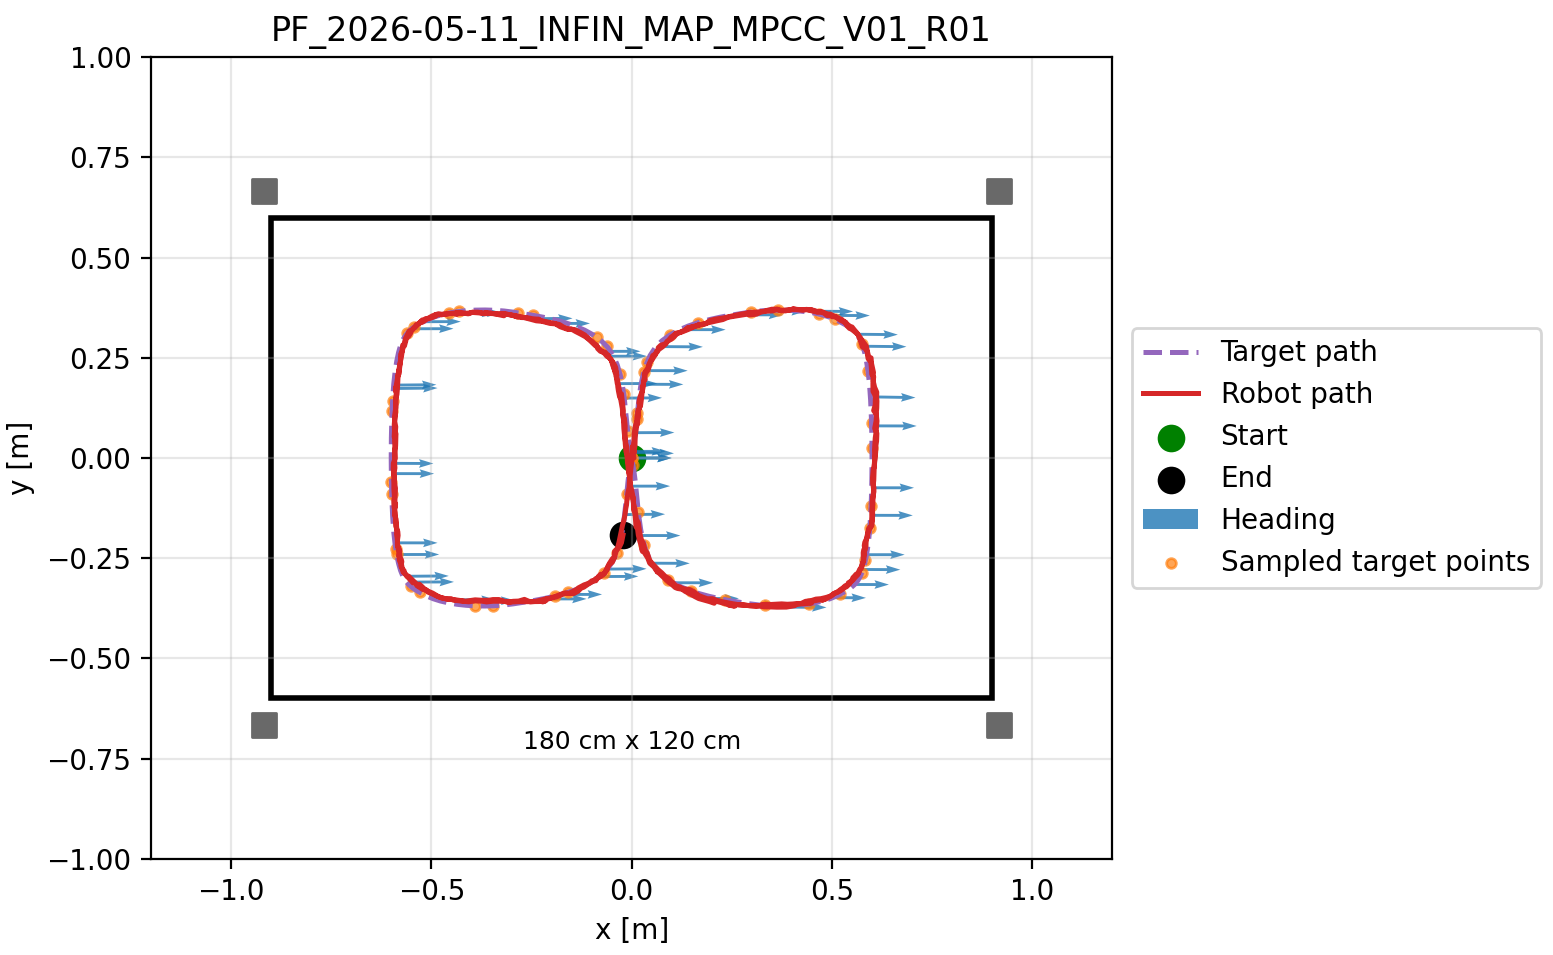
\includegraphics[width=0.7\linewidth]{IMG/controller/MPC/MPC_01_xy_map.png}
        \caption{MPC\_01 xy map}
        \label{fig:MPC_01_xy_map}
    \end{subfigure}

    \vspace{0.5em}

    \begin{subfigure}{\textwidth}
        \centering
        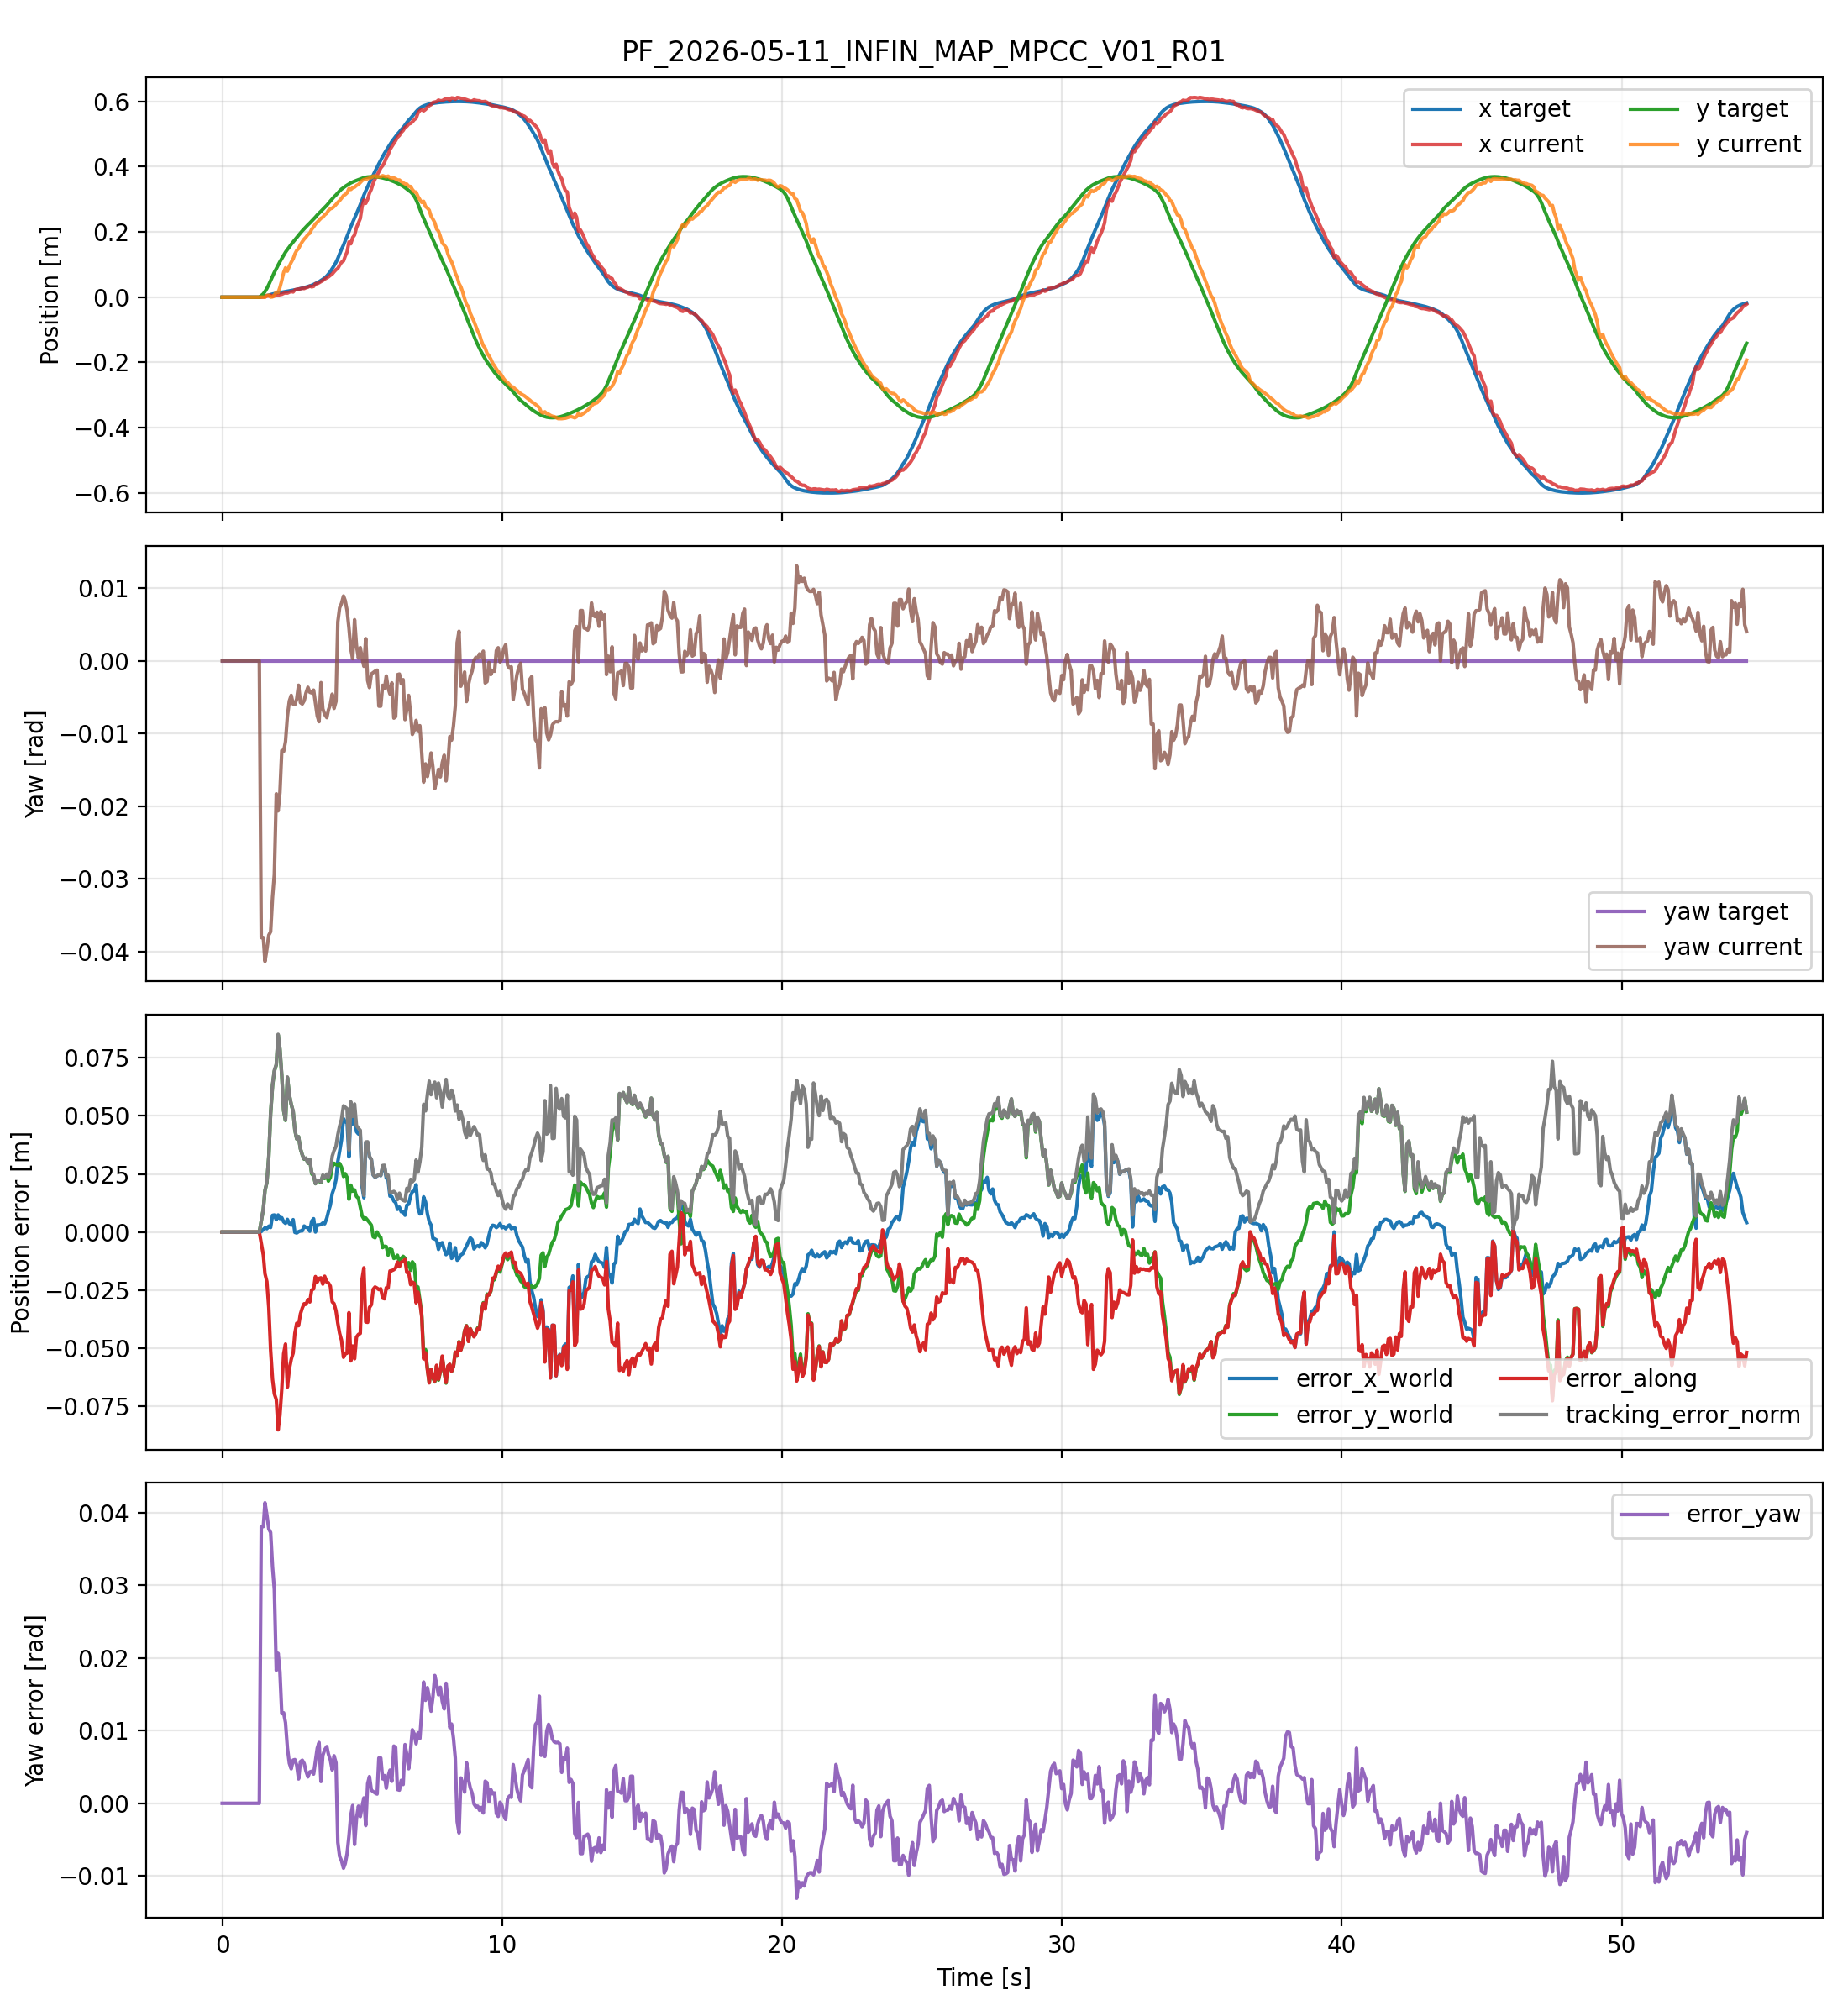
\includegraphics[width=0.7\linewidth]{IMG/controller/MPC/MPC_01_track_error.png}
        \caption{MPC\_01 tracking and errors}
        \label{fig:MPC_01_tracking_and_errors}
    \end{subfigure}
    \caption{Experimental results for MPC\_01 scenario.}
    \label{fig:MPC_01_general}
\end{figure}

\newpage
\begin{figure}[H]
    \centering
    \begin{subfigure}{\textwidth}
        \centering
        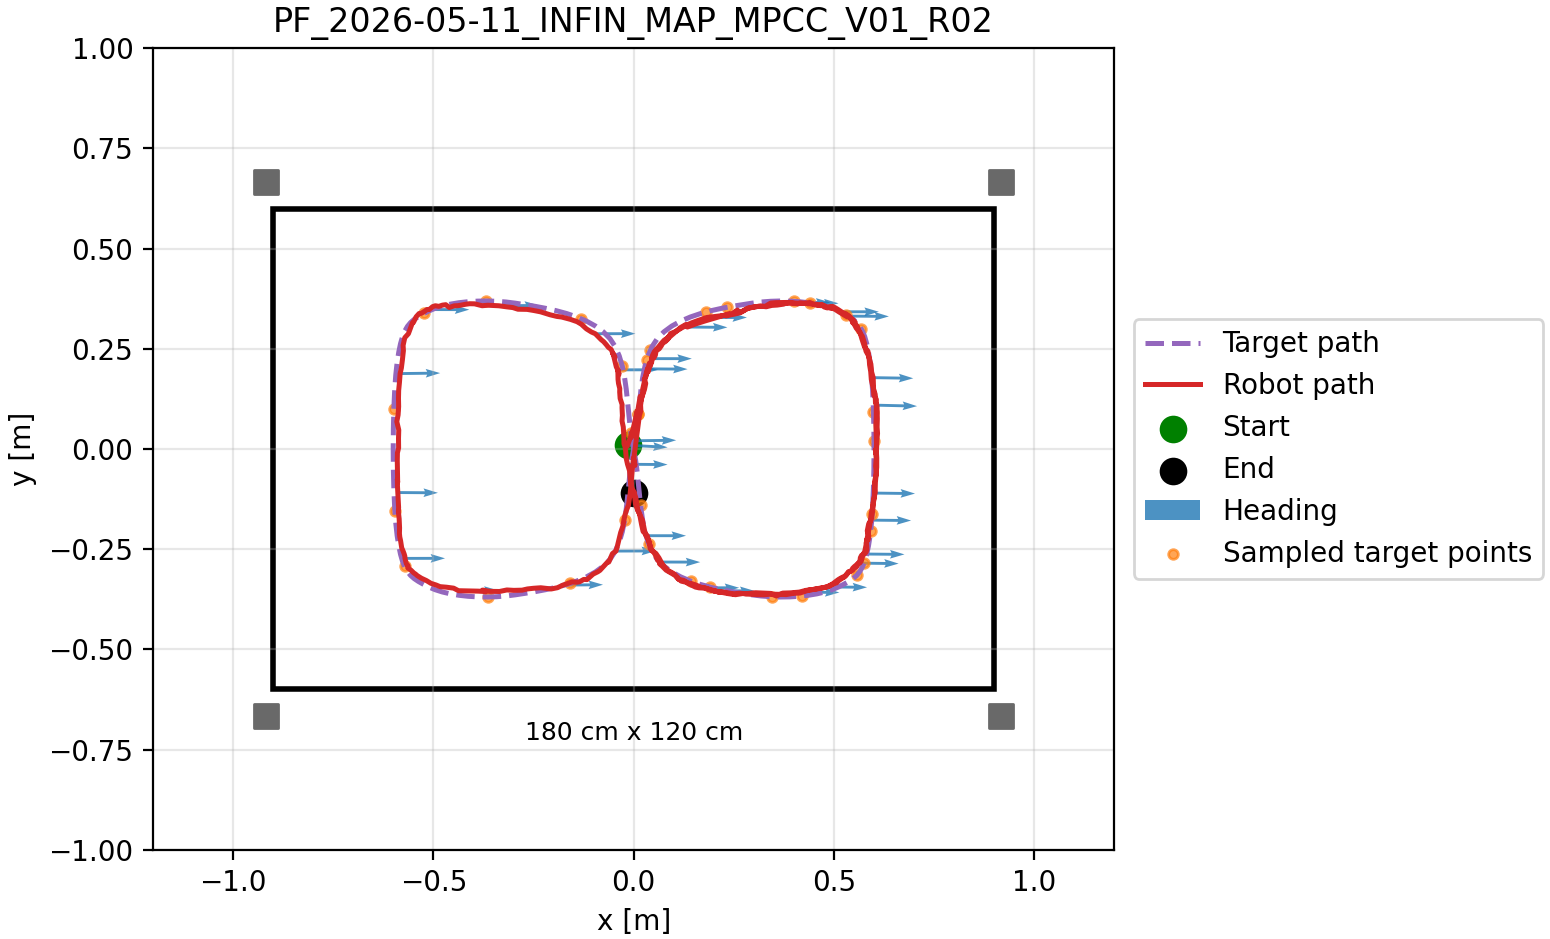
\includegraphics[width=0.7\linewidth]{IMG/controller/MPC/MPC_02_xy_map.png}
        \caption{MPC\_02 xy map}
        \label{fig:MPC_02_xy_map}
    \end{subfigure}

    \vspace{0.5em}

    \begin{subfigure}{\textwidth}
        \centering
        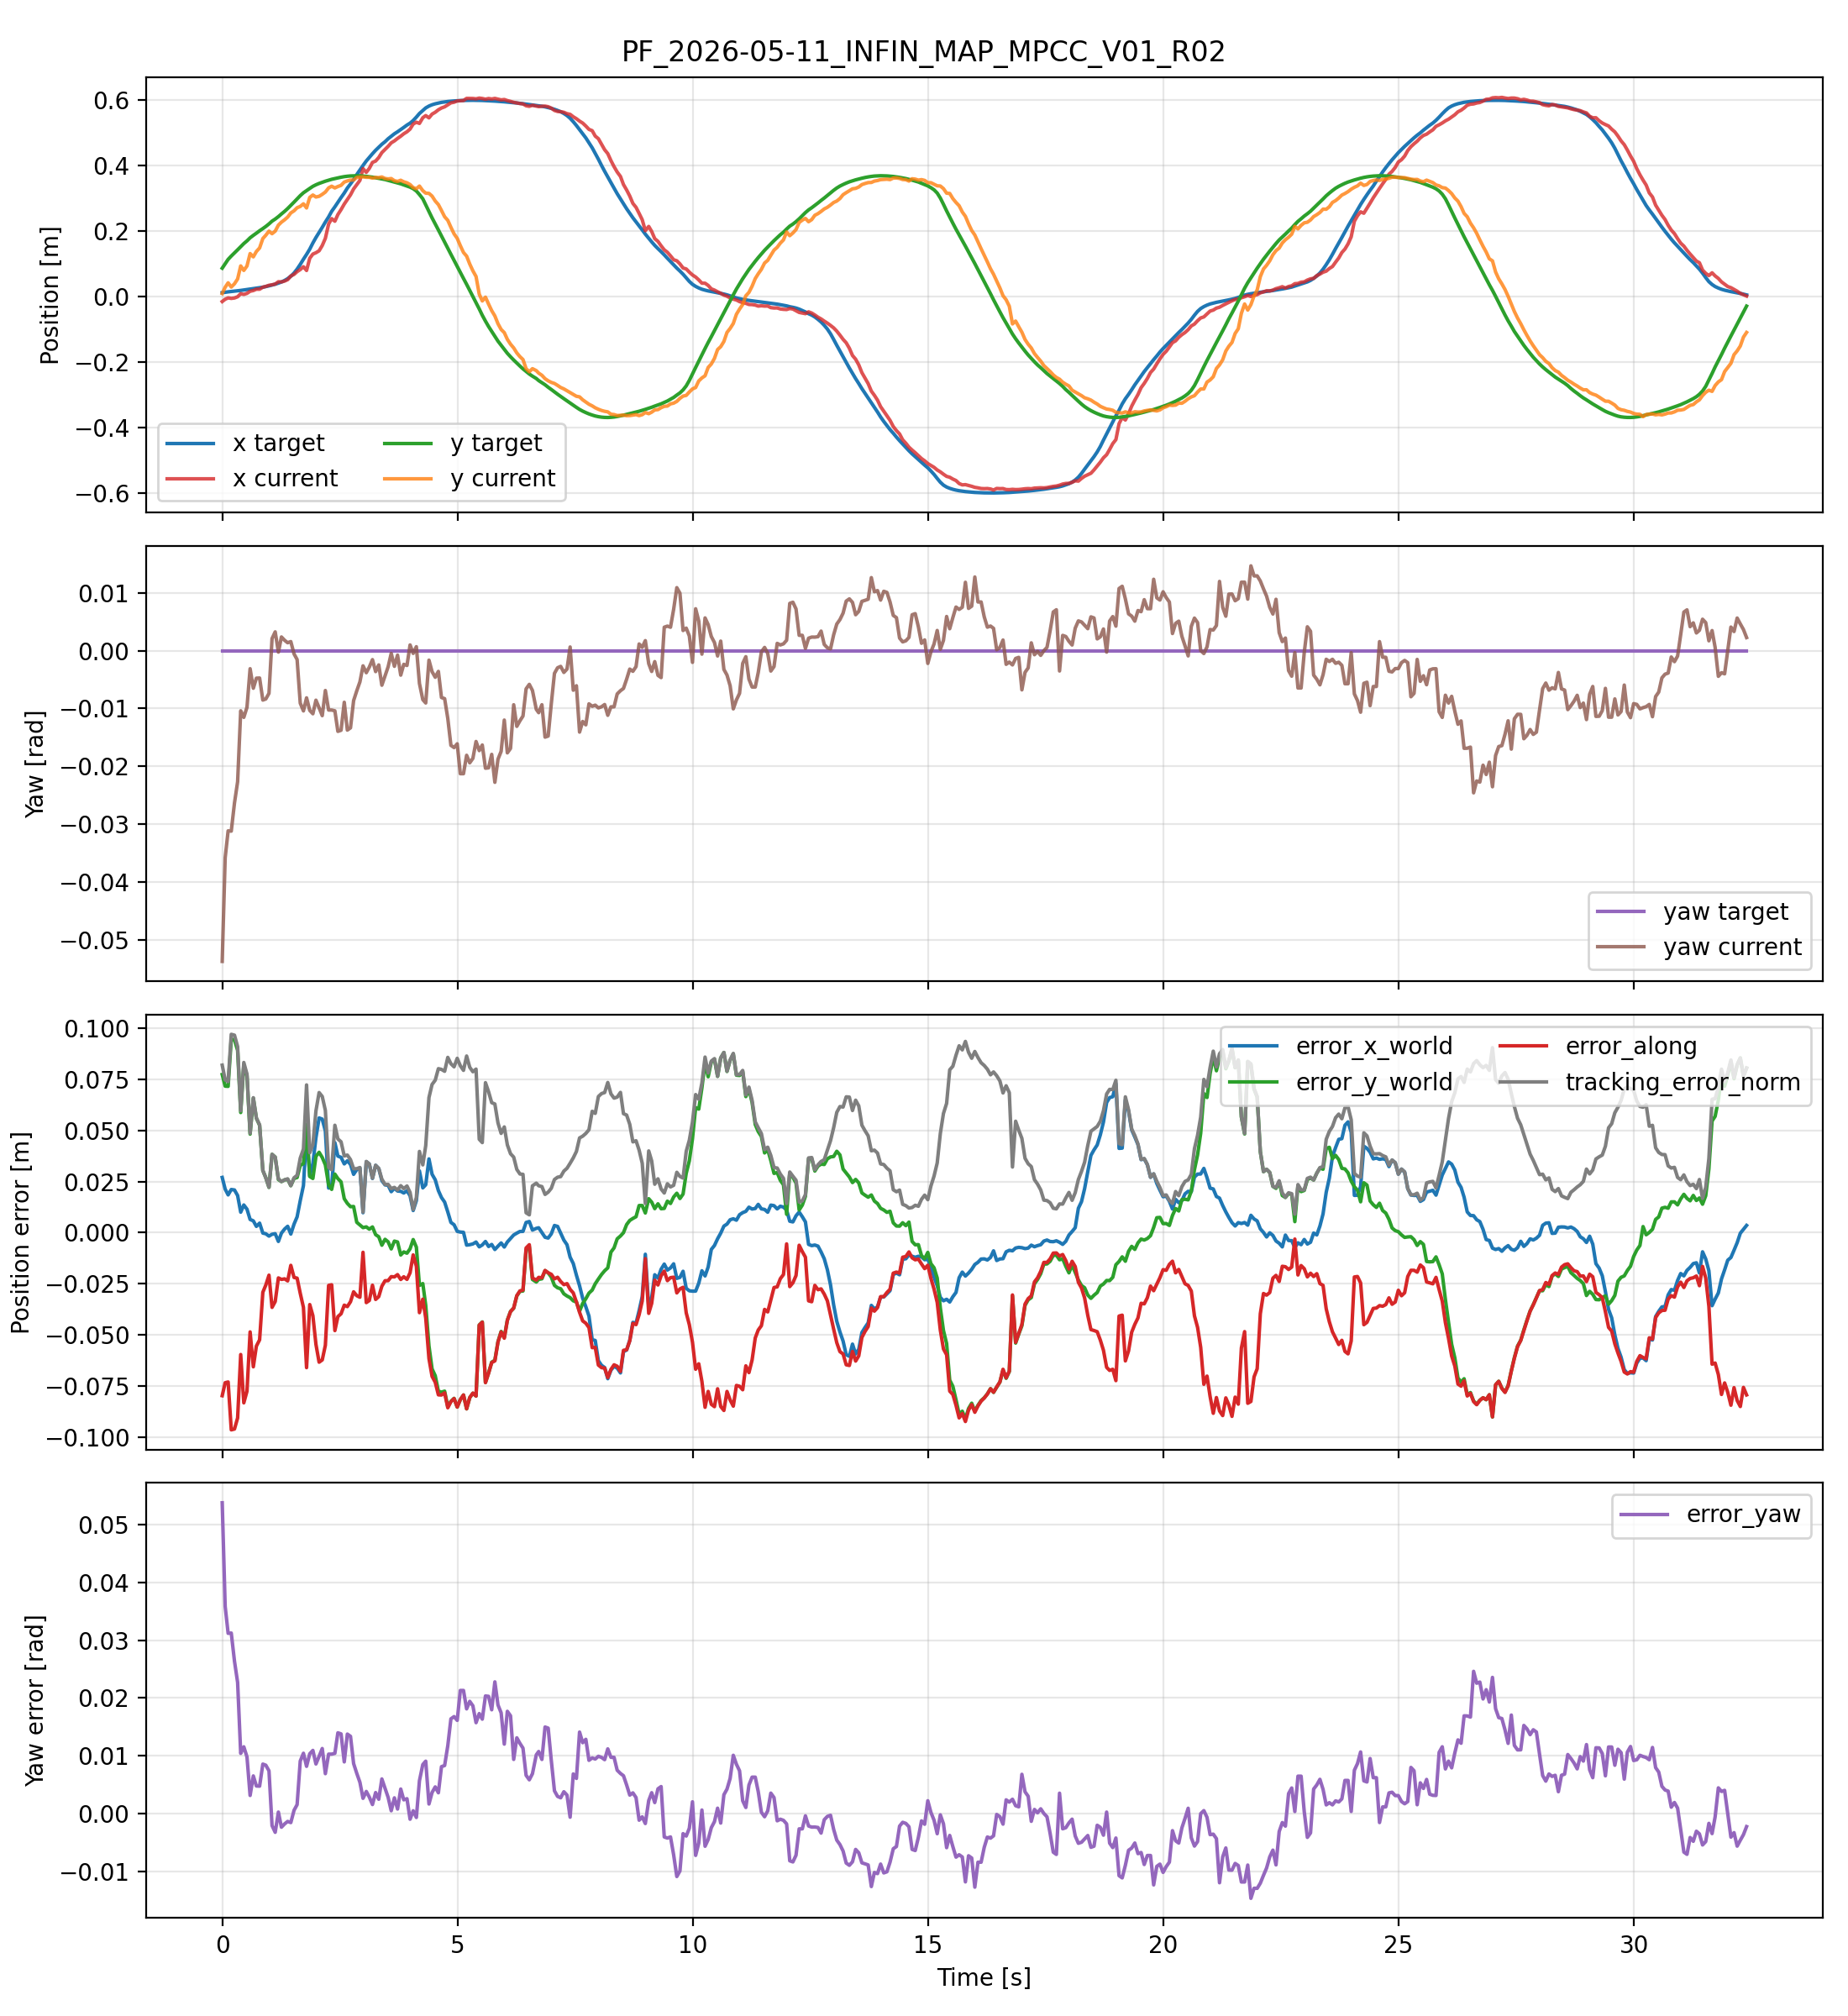
\includegraphics[width=0.7\linewidth]{IMG/controller/MPC/MPC_02_track_error.png}
        \caption{MPC\_02 tracking and errors}
        \label{fig:MPC_02_tracking_and_errors}
    \end{subfigure}
    \caption{Experimental results for MPC\_02 scenario.}
    \label{fig:MPC_02_general}
\end{figure}

\newpage
\begin{figure}[H]
    \centering
    \begin{subfigure}{\textwidth}
        \centering
        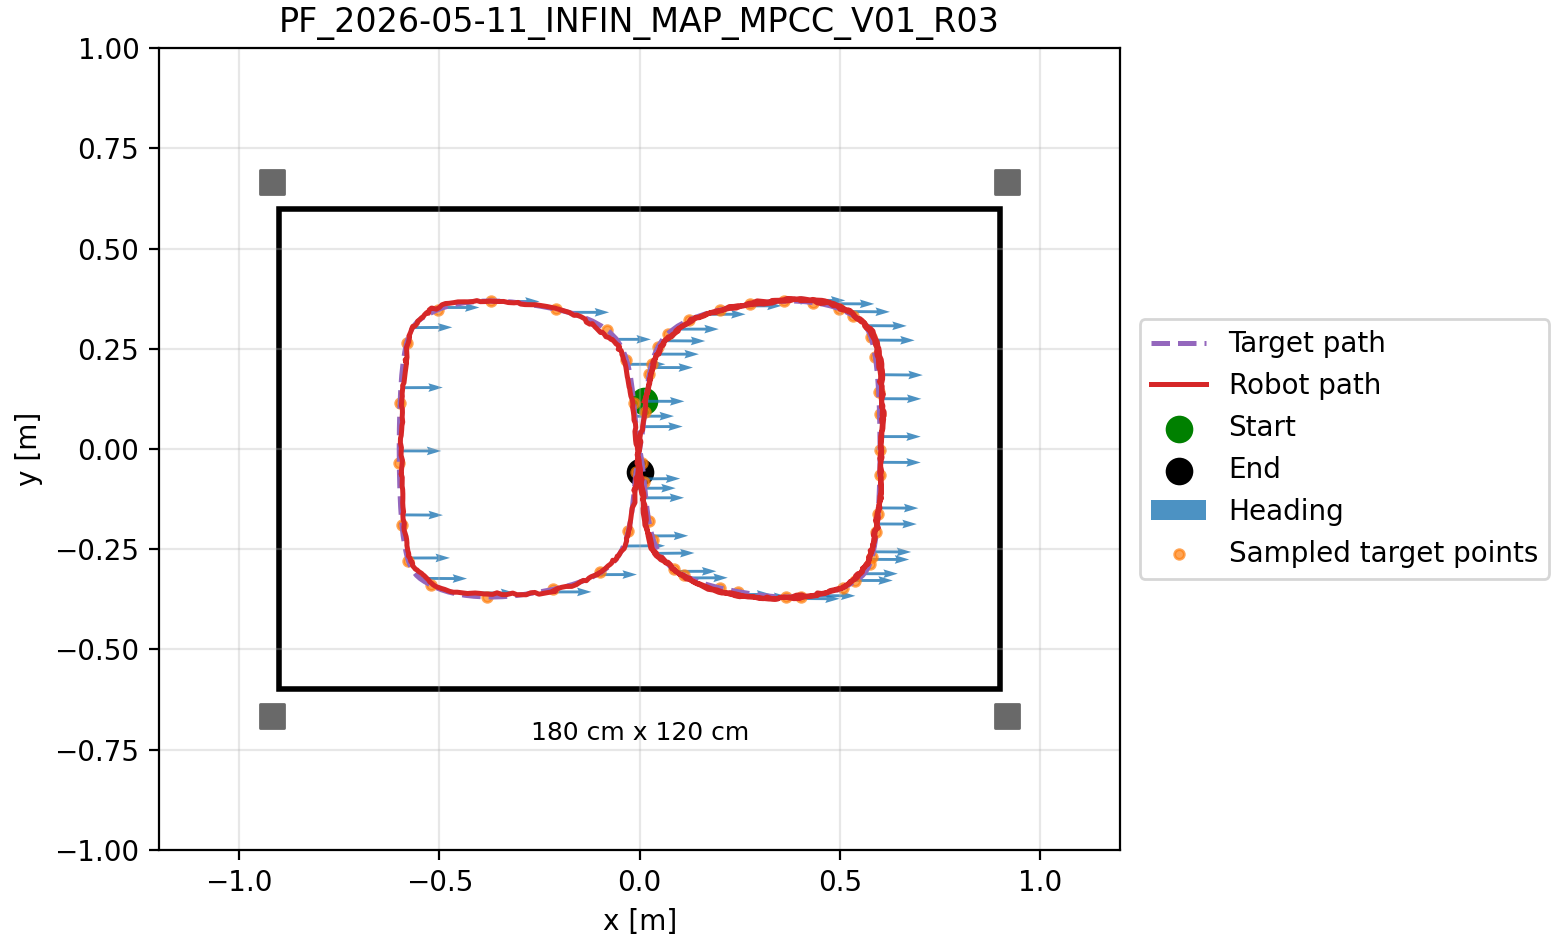
\includegraphics[width=0.7\linewidth]{IMG/controller/MPC/MPC_03_xy_map.png}
        \caption{MPC\_03 xy map}
        \label{fig:MPC_03_xy_map}
    \end{subfigure}

    \vspace{0.5em}

    \begin{subfigure}{\textwidth}
        \centering
        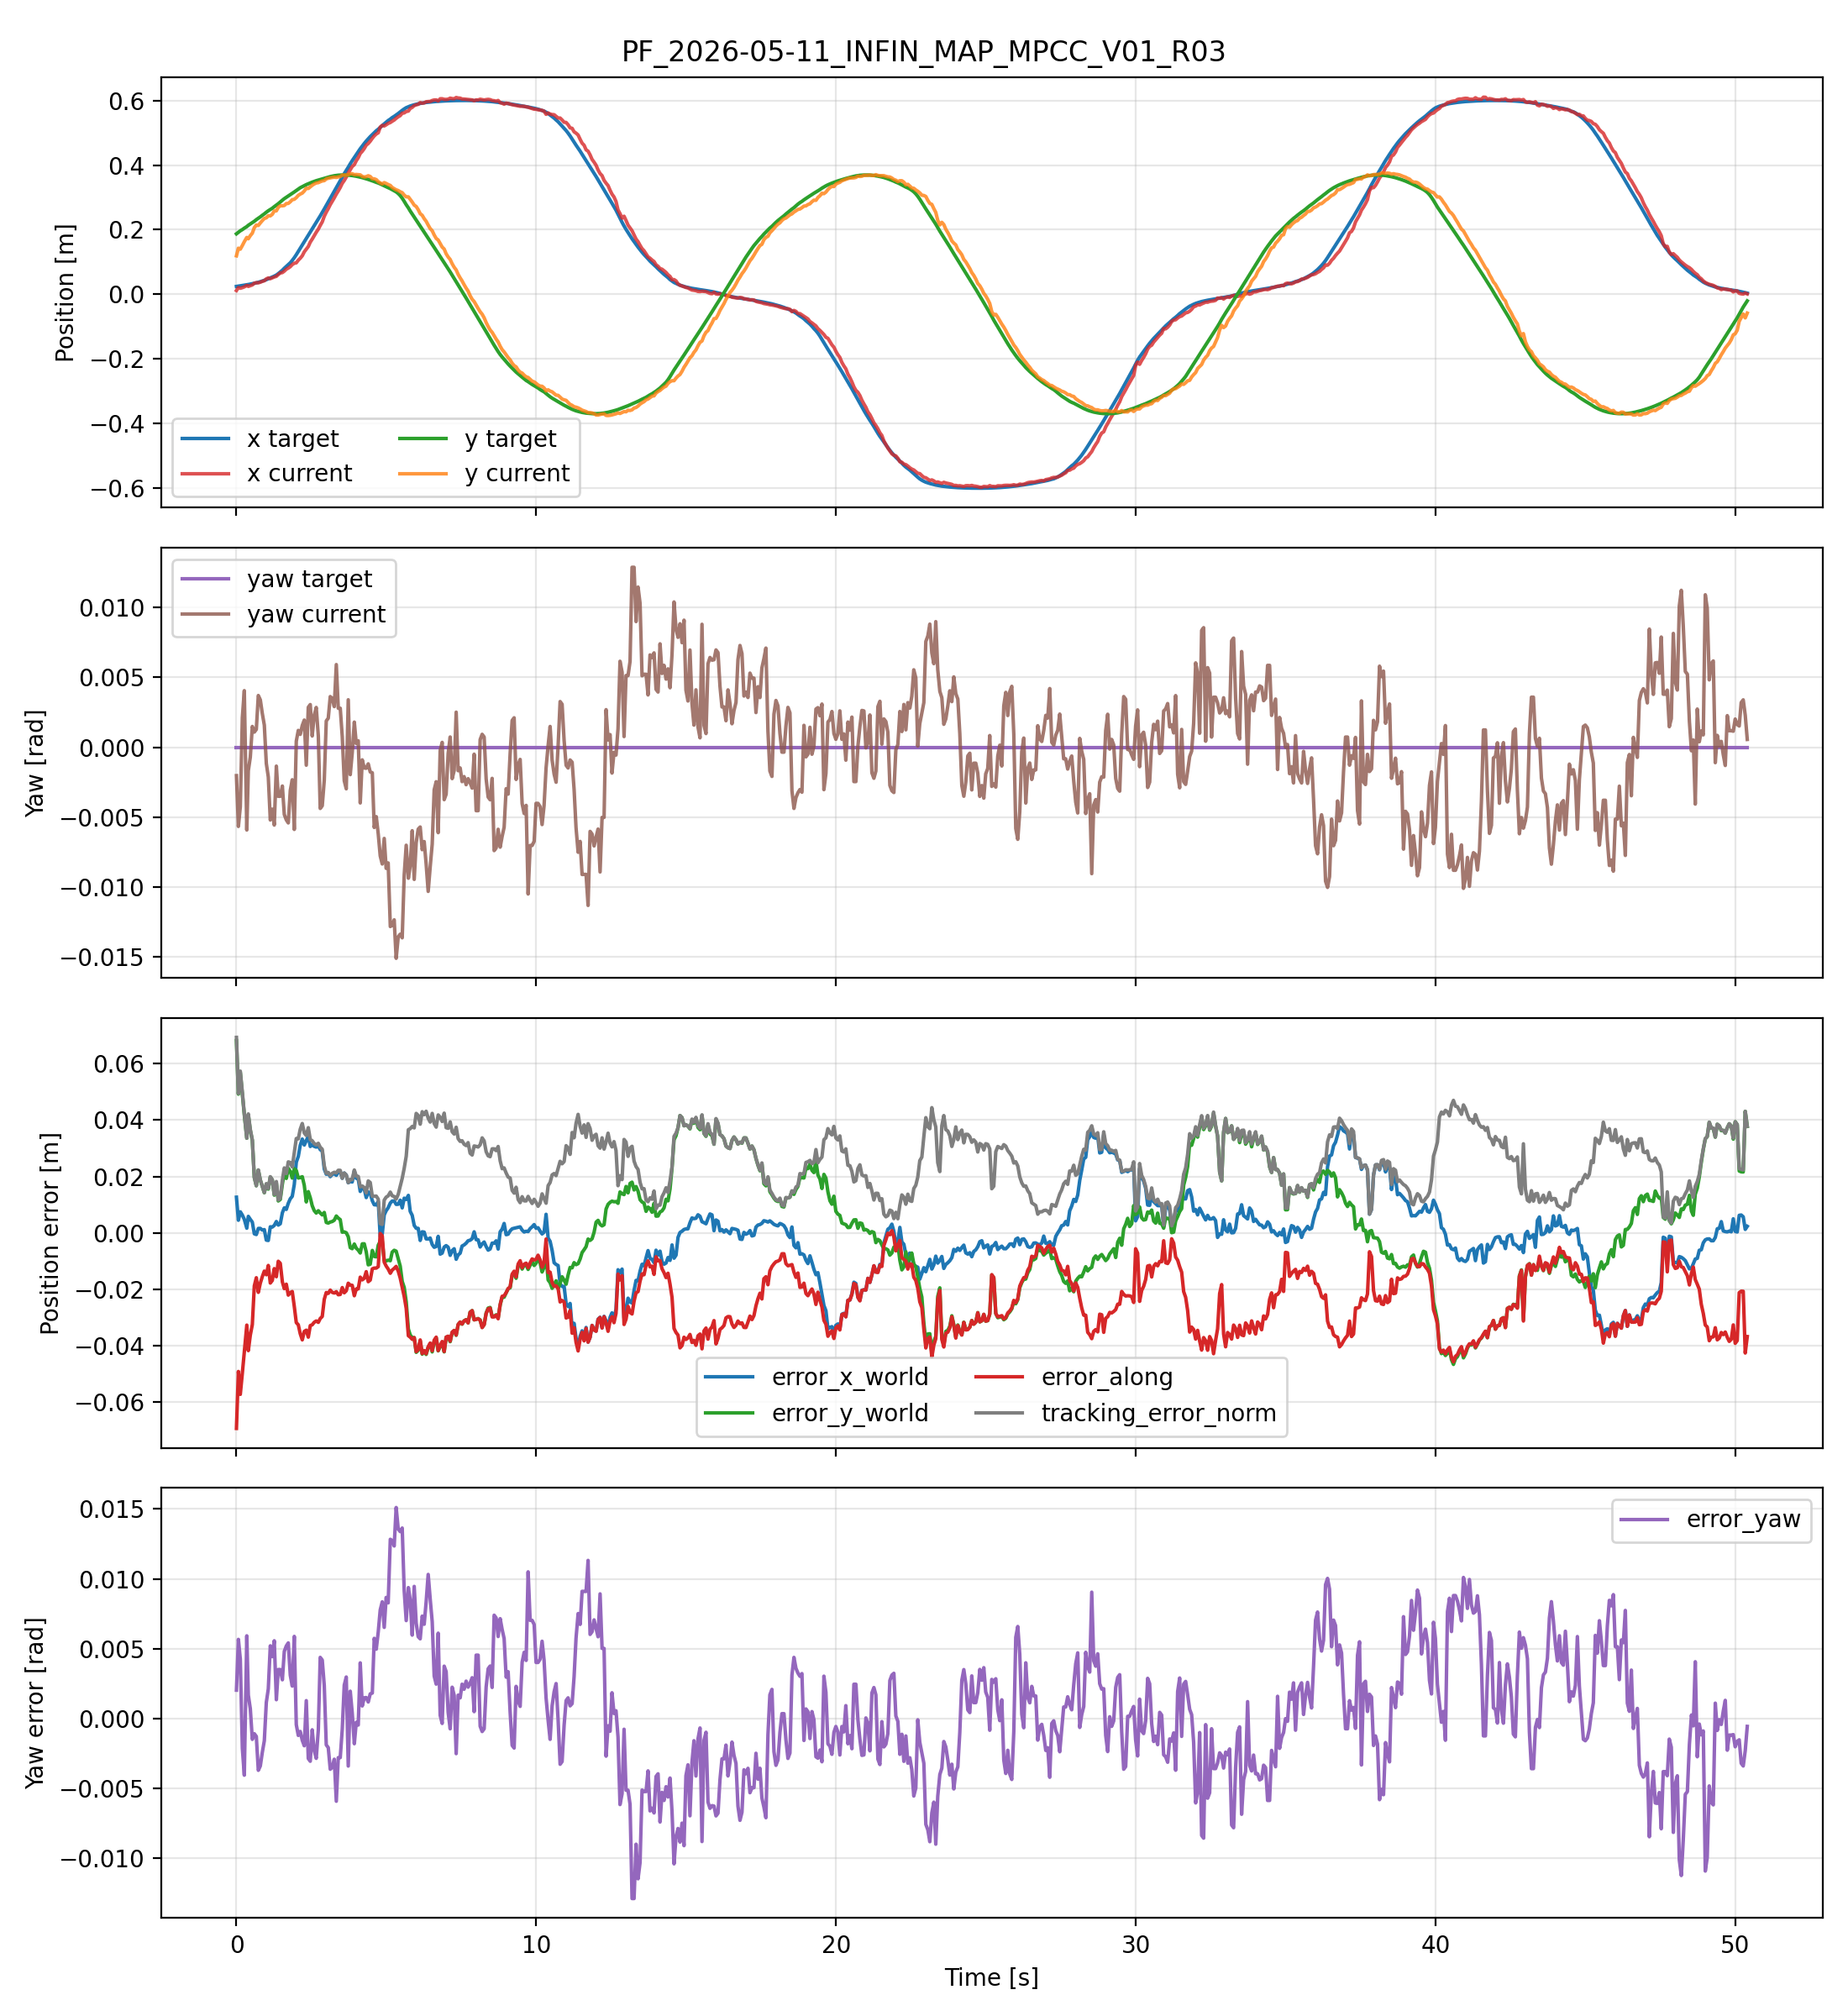
\includegraphics[width=0.7\linewidth]{IMG/controller/MPC/MPC_03_track_error.png}
        \caption{MPC\_03 tracking and errors}
        \label{fig:MPC_03_tracking_and_errors}
    \end{subfigure}
    \caption{Experimental results for MPC\_03 scenario.}
    \label{fig:MPC_03_general}
\end{figure}

\newpage
\begin{figure}[H]
    \centering
    \begin{subfigure}{\textwidth}
        \centering
        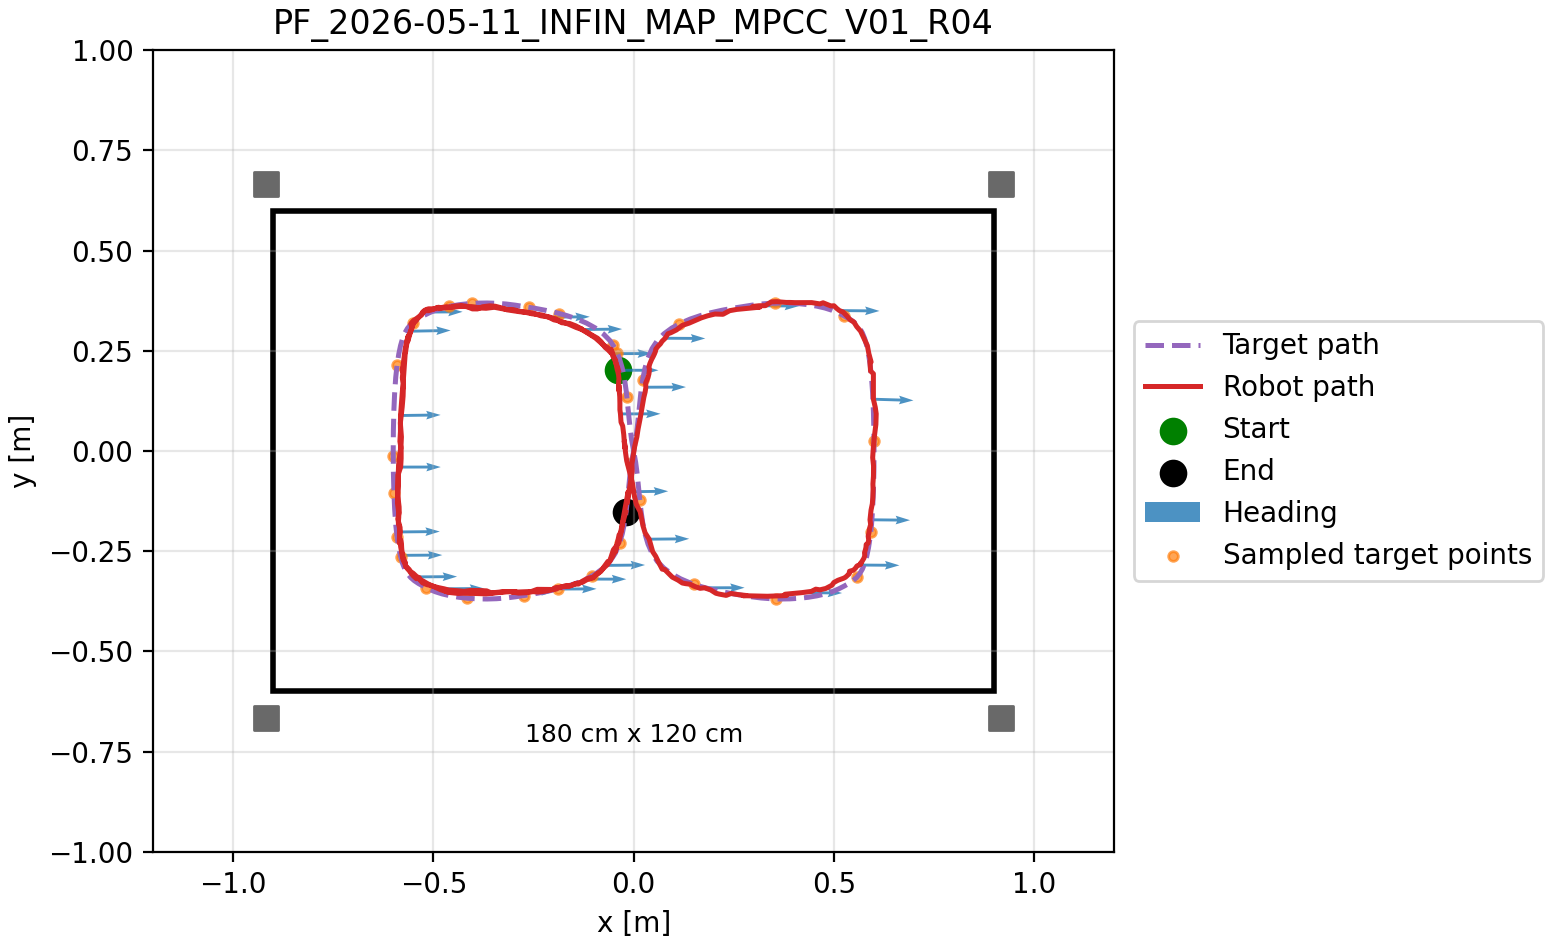
\includegraphics[width=0.7\linewidth]{IMG/controller/MPC/MPC_04_xy_map.png}
        \caption{MPC\_04 xy map}
        \label{fig:MPC_04_xy_map}
    \end{subfigure}

    \vspace{0.5em}

    \begin{subfigure}{\textwidth}
        \centering
        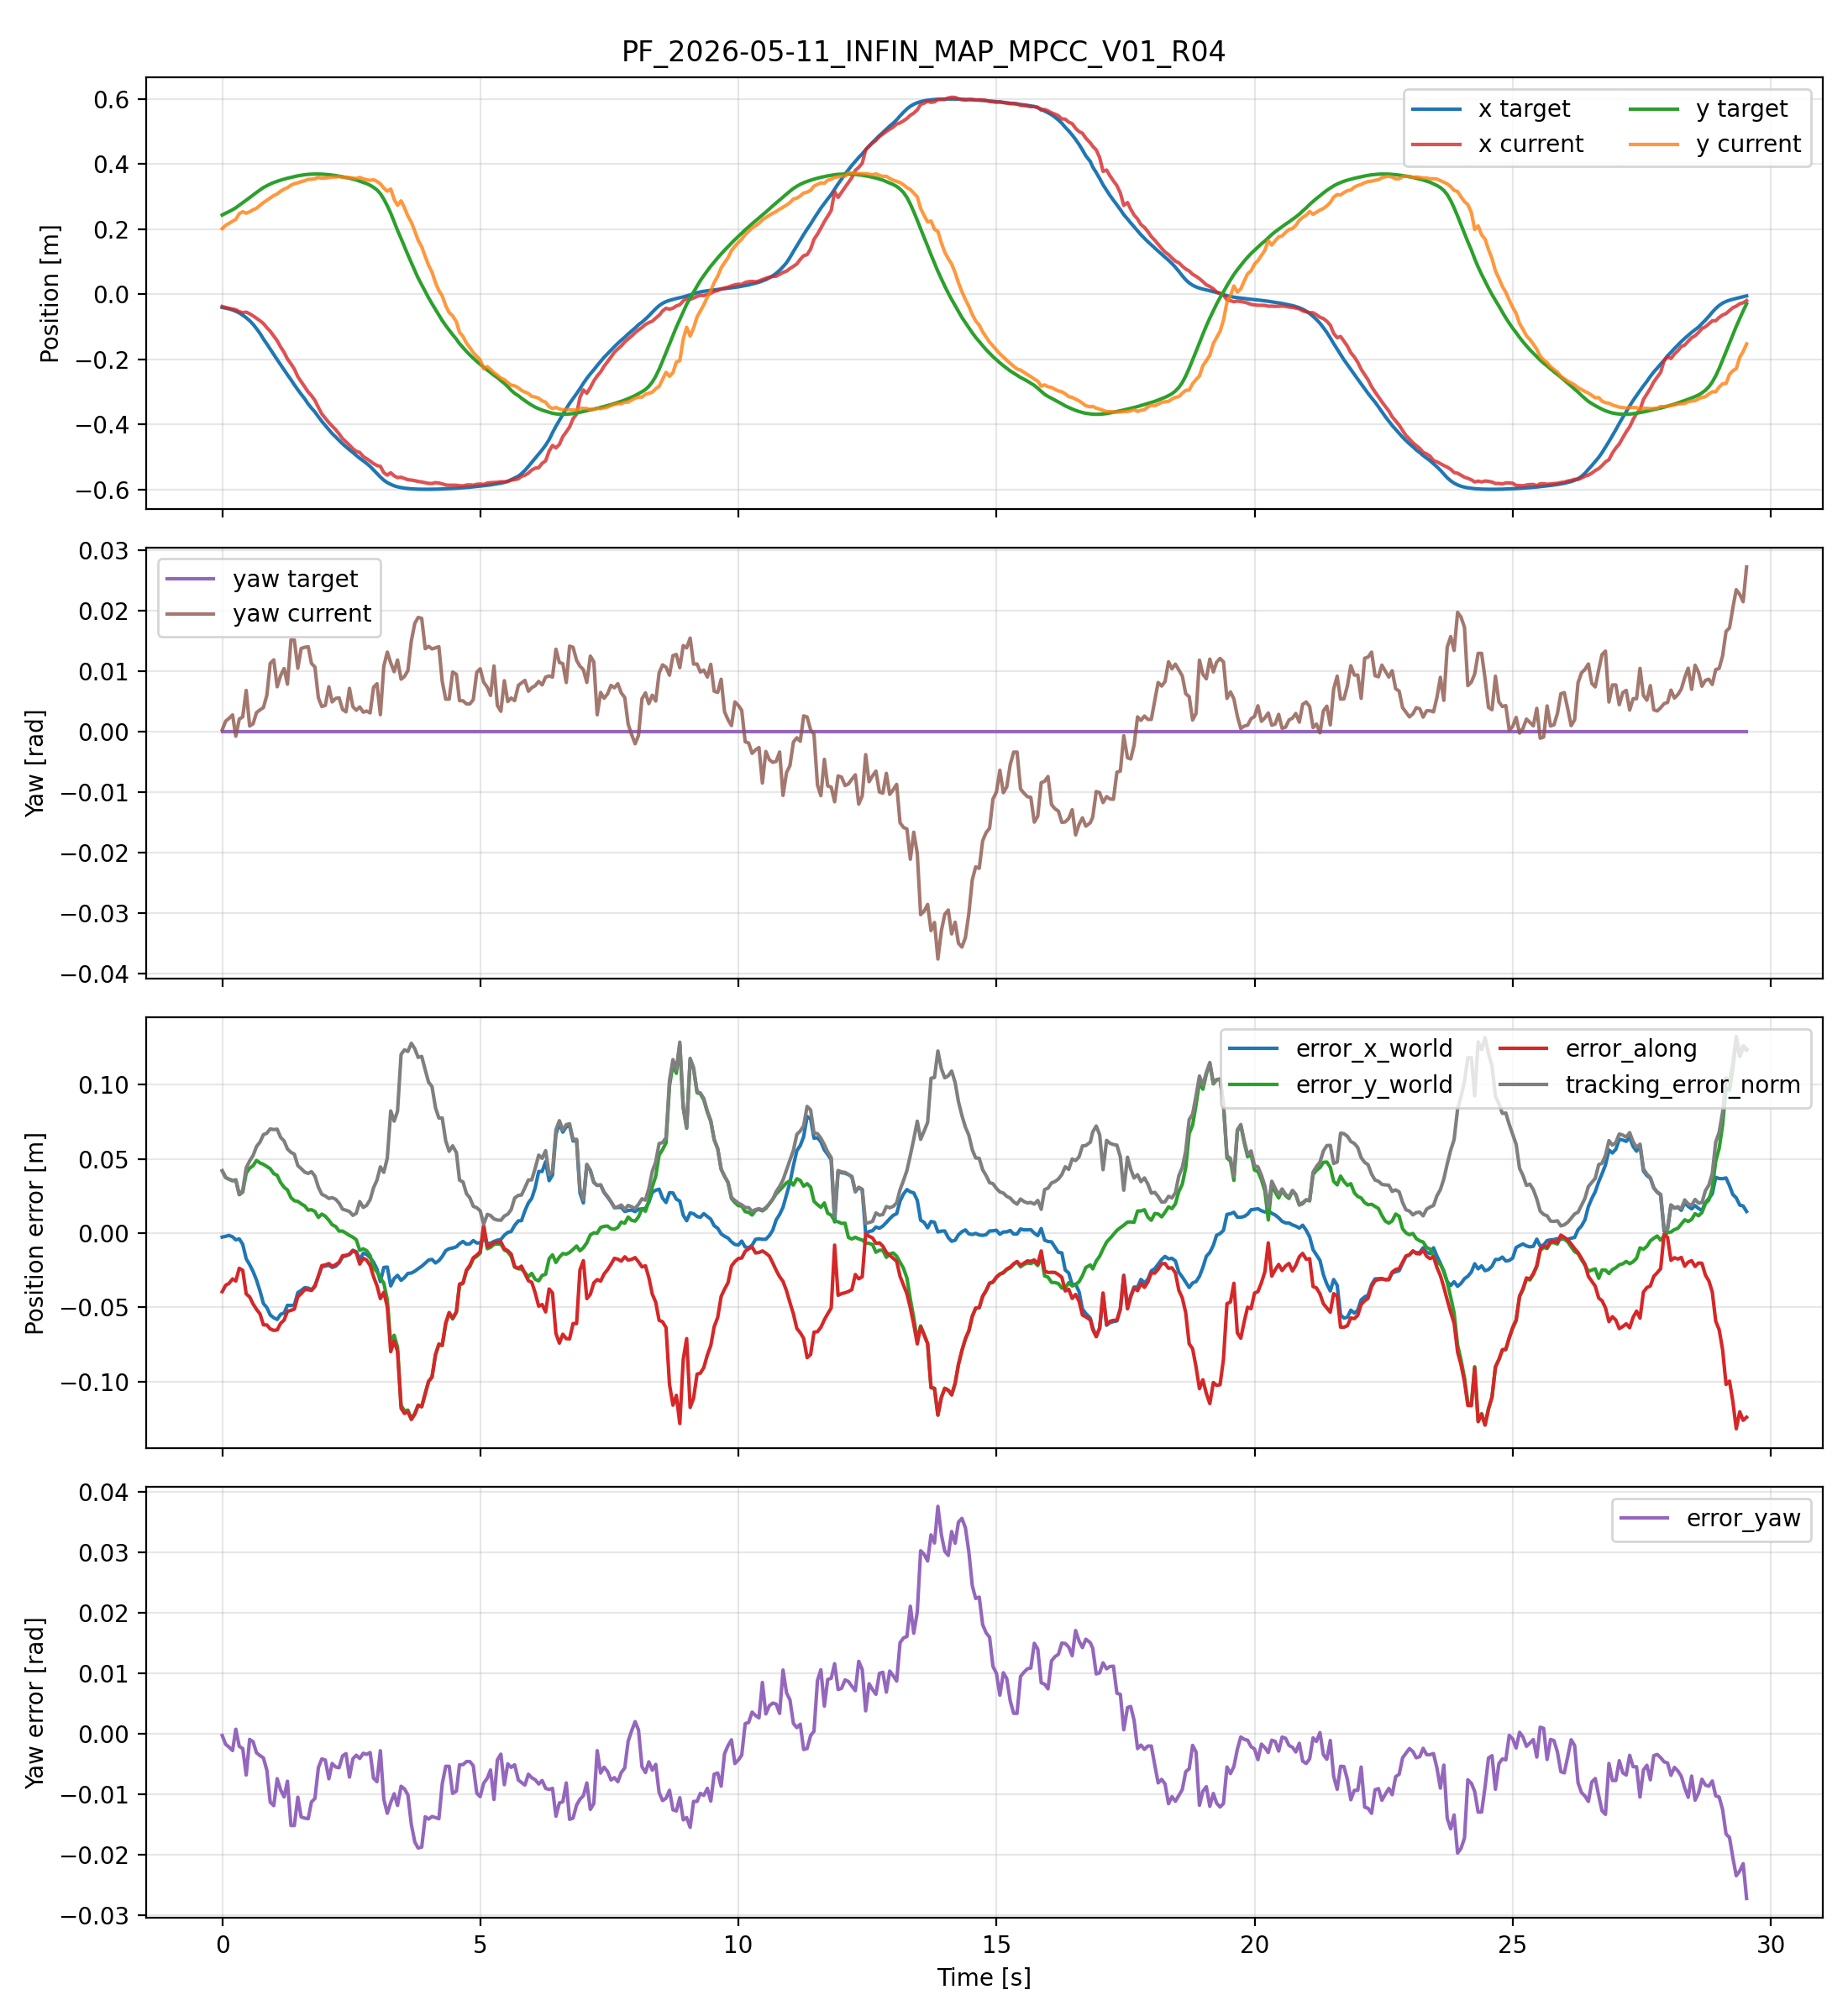
\includegraphics[width=0.7\linewidth]{IMG/controller/MPC/MPC_04_track_error.png}
        \caption{MPC\_04 tracking and errors}
        \label{fig:MPC_04_tracking_and_errors}
    \end{subfigure}
    \caption{Experimental results for MPC\_04 scenario.}
    \label{fig:MPC_04_general}
\end{figure}

\newpage
\begin{figure}[H]
    \centering
    \begin{subfigure}{\textwidth}
        \centering
        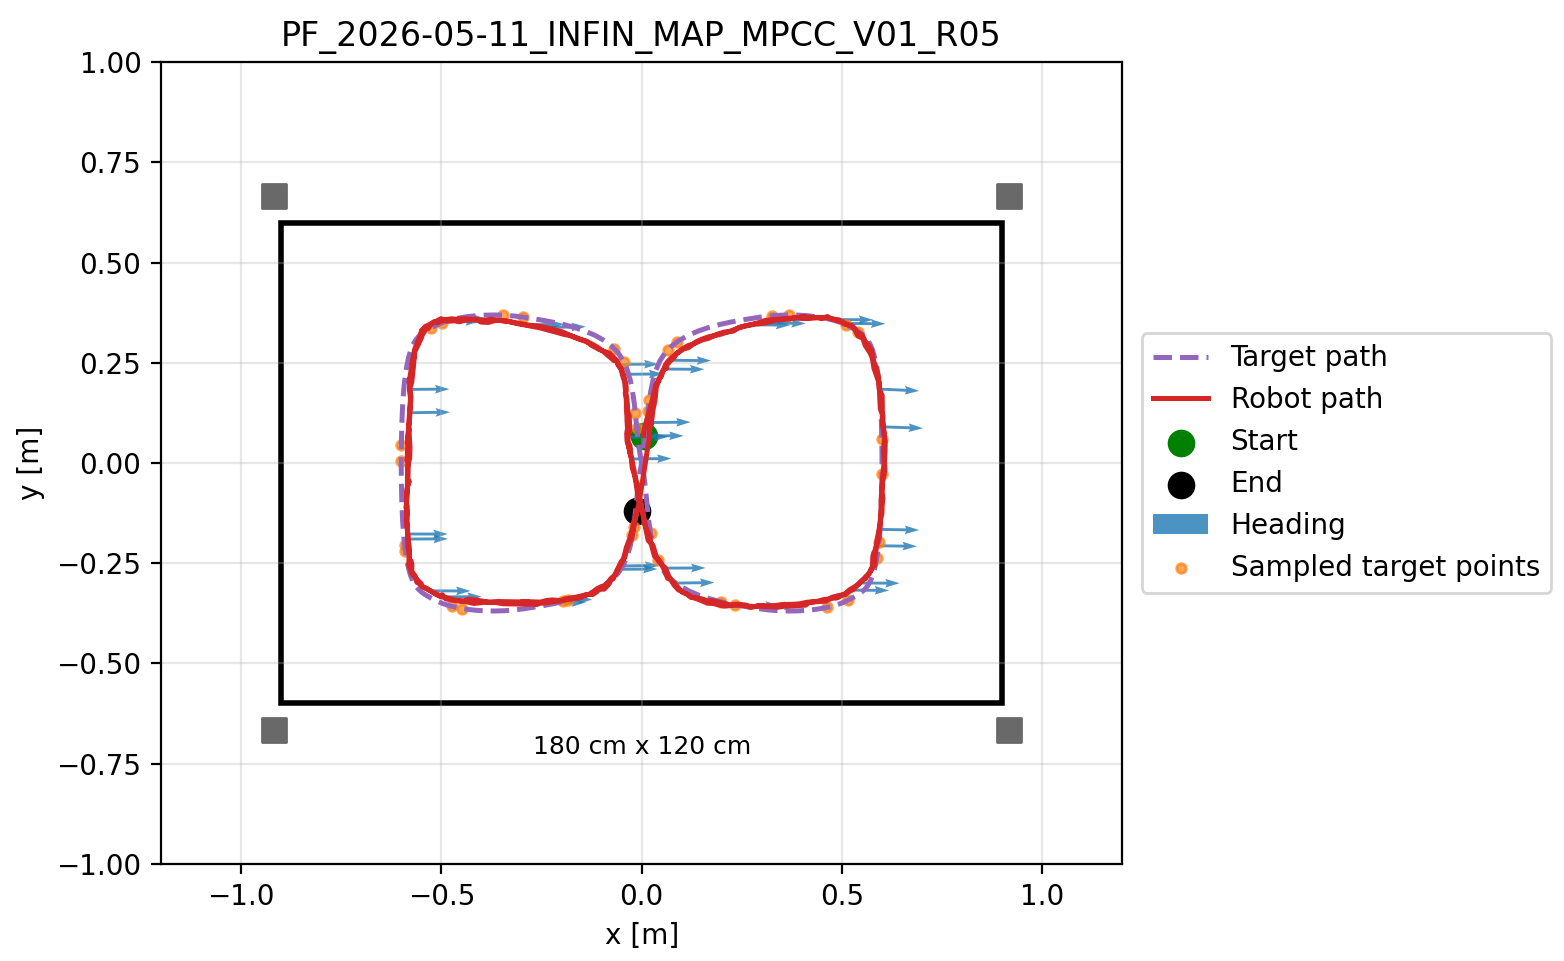
\includegraphics[width=0.7\linewidth]{IMG/controller/MPC/MPC_05_xy_map.png}
        \caption{MPC\_05 xy map}
        \label{fig:MPC_05_xy_map}
    \end{subfigure}

    \vspace{0.5em}

    \begin{subfigure}{\textwidth}
        \centering
        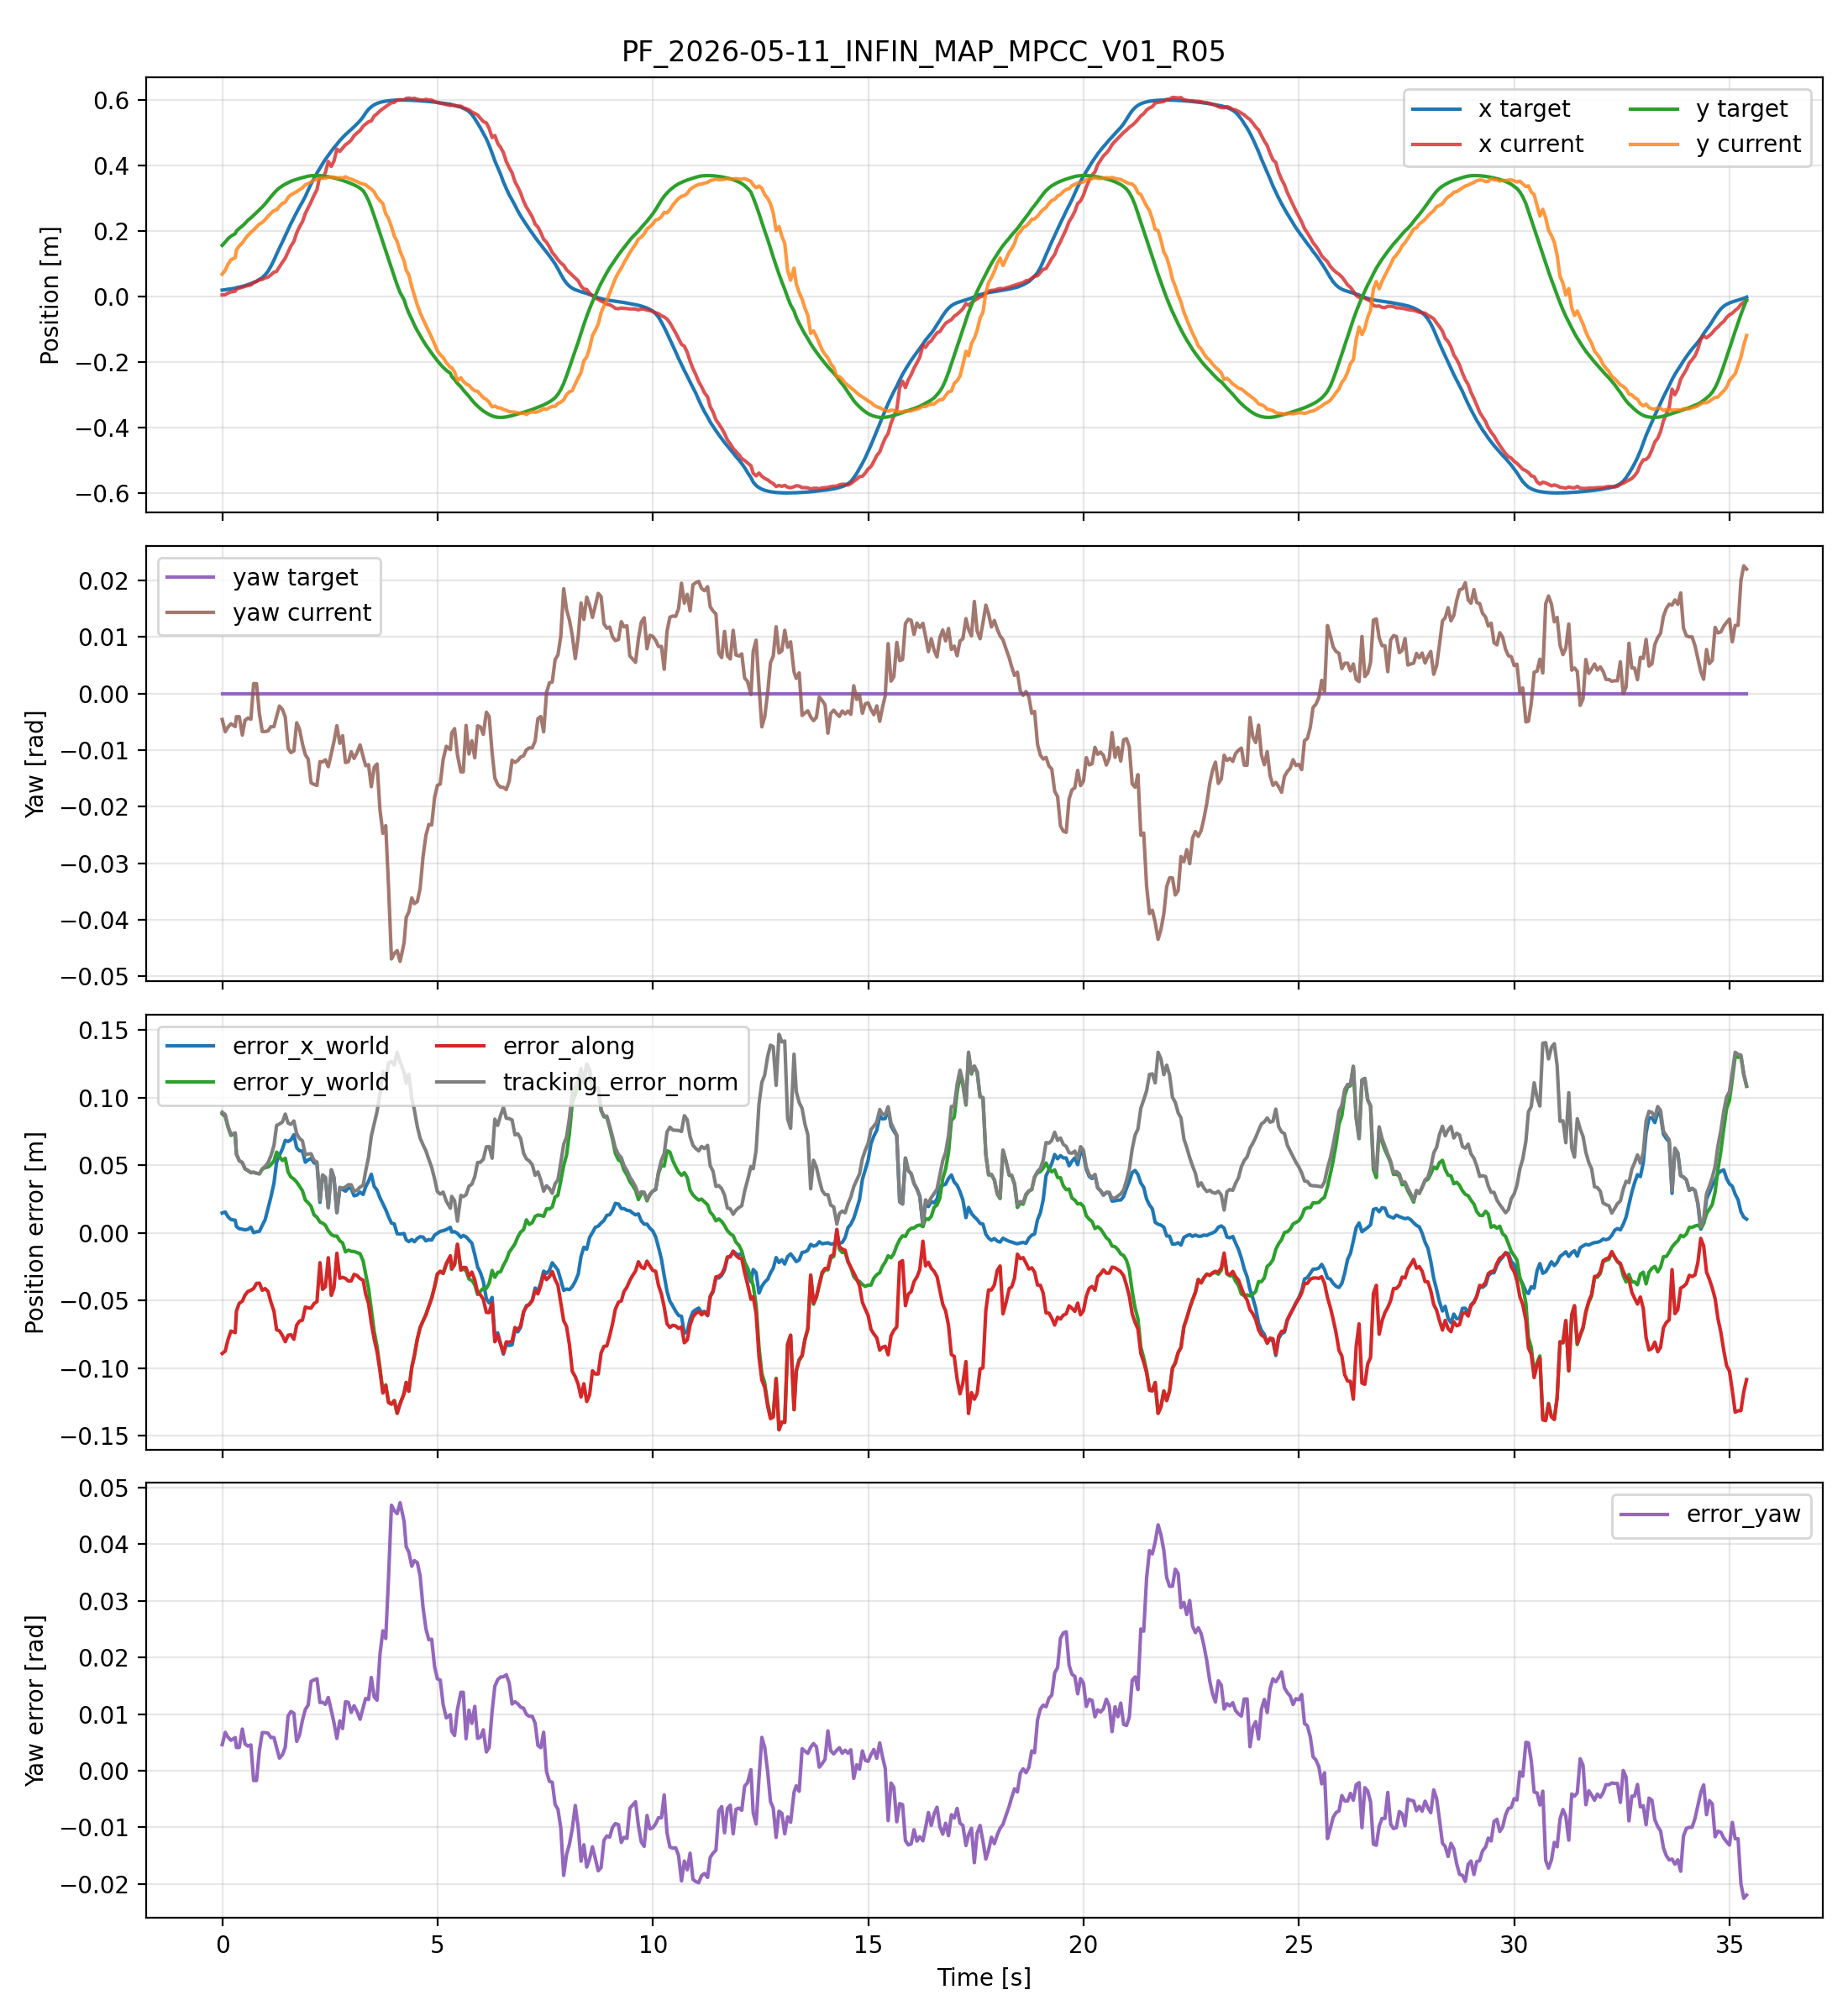
\includegraphics[width=0.7\linewidth]{IMG/controller/MPC/MPC_05_track_error.png}
        \caption{MPC\_05 tracking and errors}
        \label{fig:MPC_05_tracking_and_errors}
    \end{subfigure}
    \caption{Experimental results for MPC\_05 scenario.}
    \label{fig:MPC_05_general}
\end{figure}

\newpage
\begin{figure}[H]
    \centering
    \begin{subfigure}{\textwidth}
        \centering
        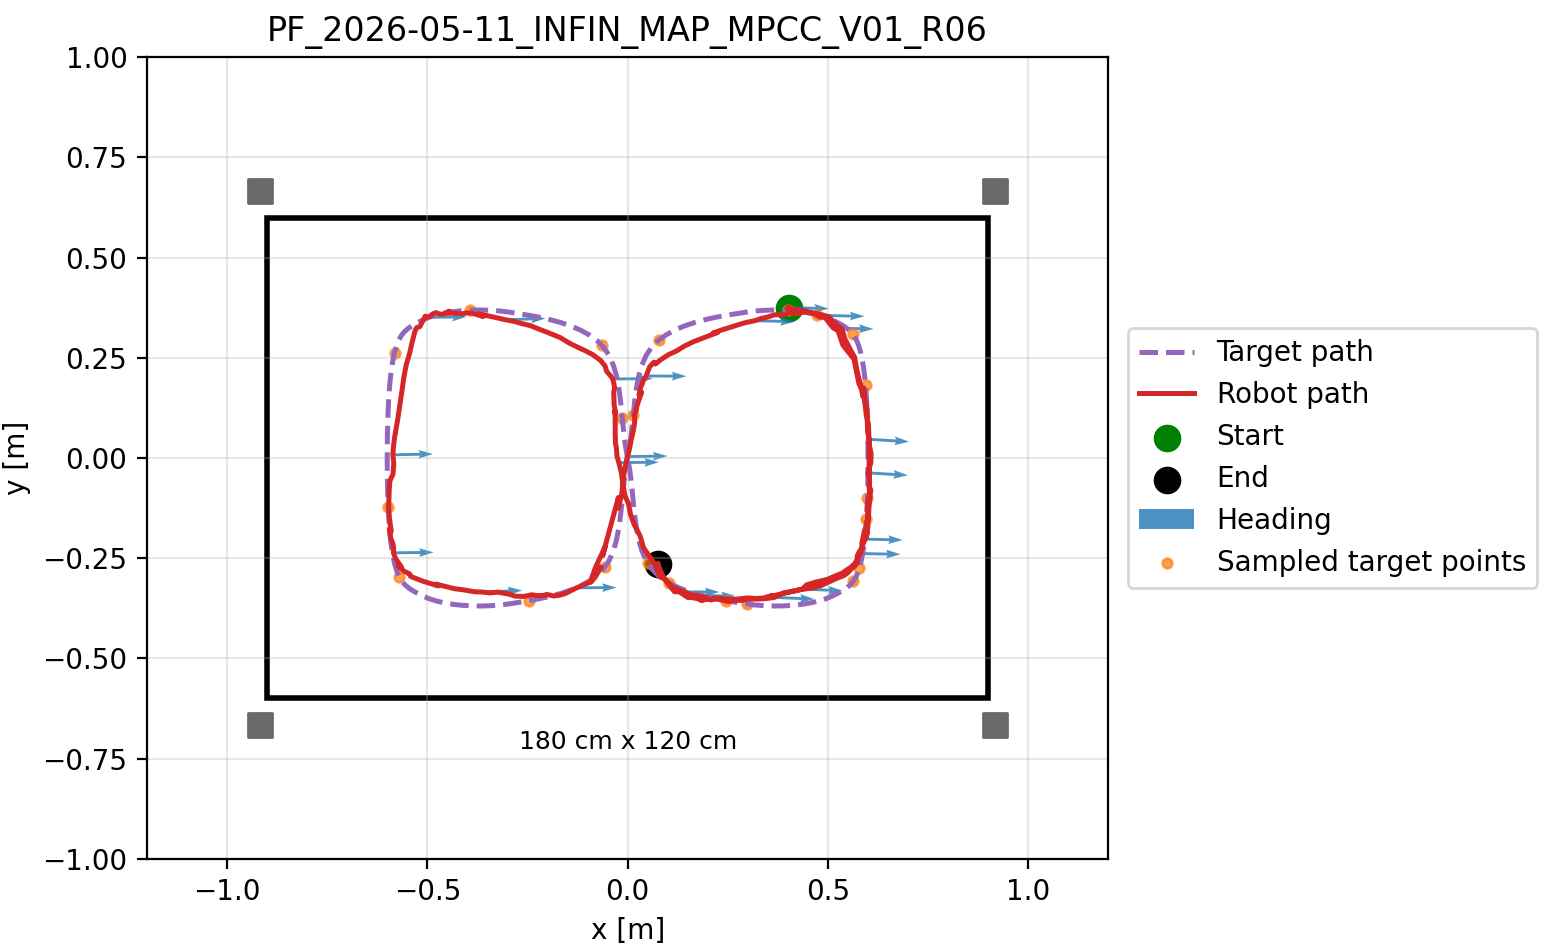
\includegraphics[width=0.7\linewidth]{IMG/controller/MPC/MPC_06_xy_map.png}
        \caption{MPC\_06 xy map}
        \label{fig:MPC_06_xy_map}
    \end{subfigure}

    \vspace{0.5em}

    \begin{subfigure}{\textwidth}
        \centering
        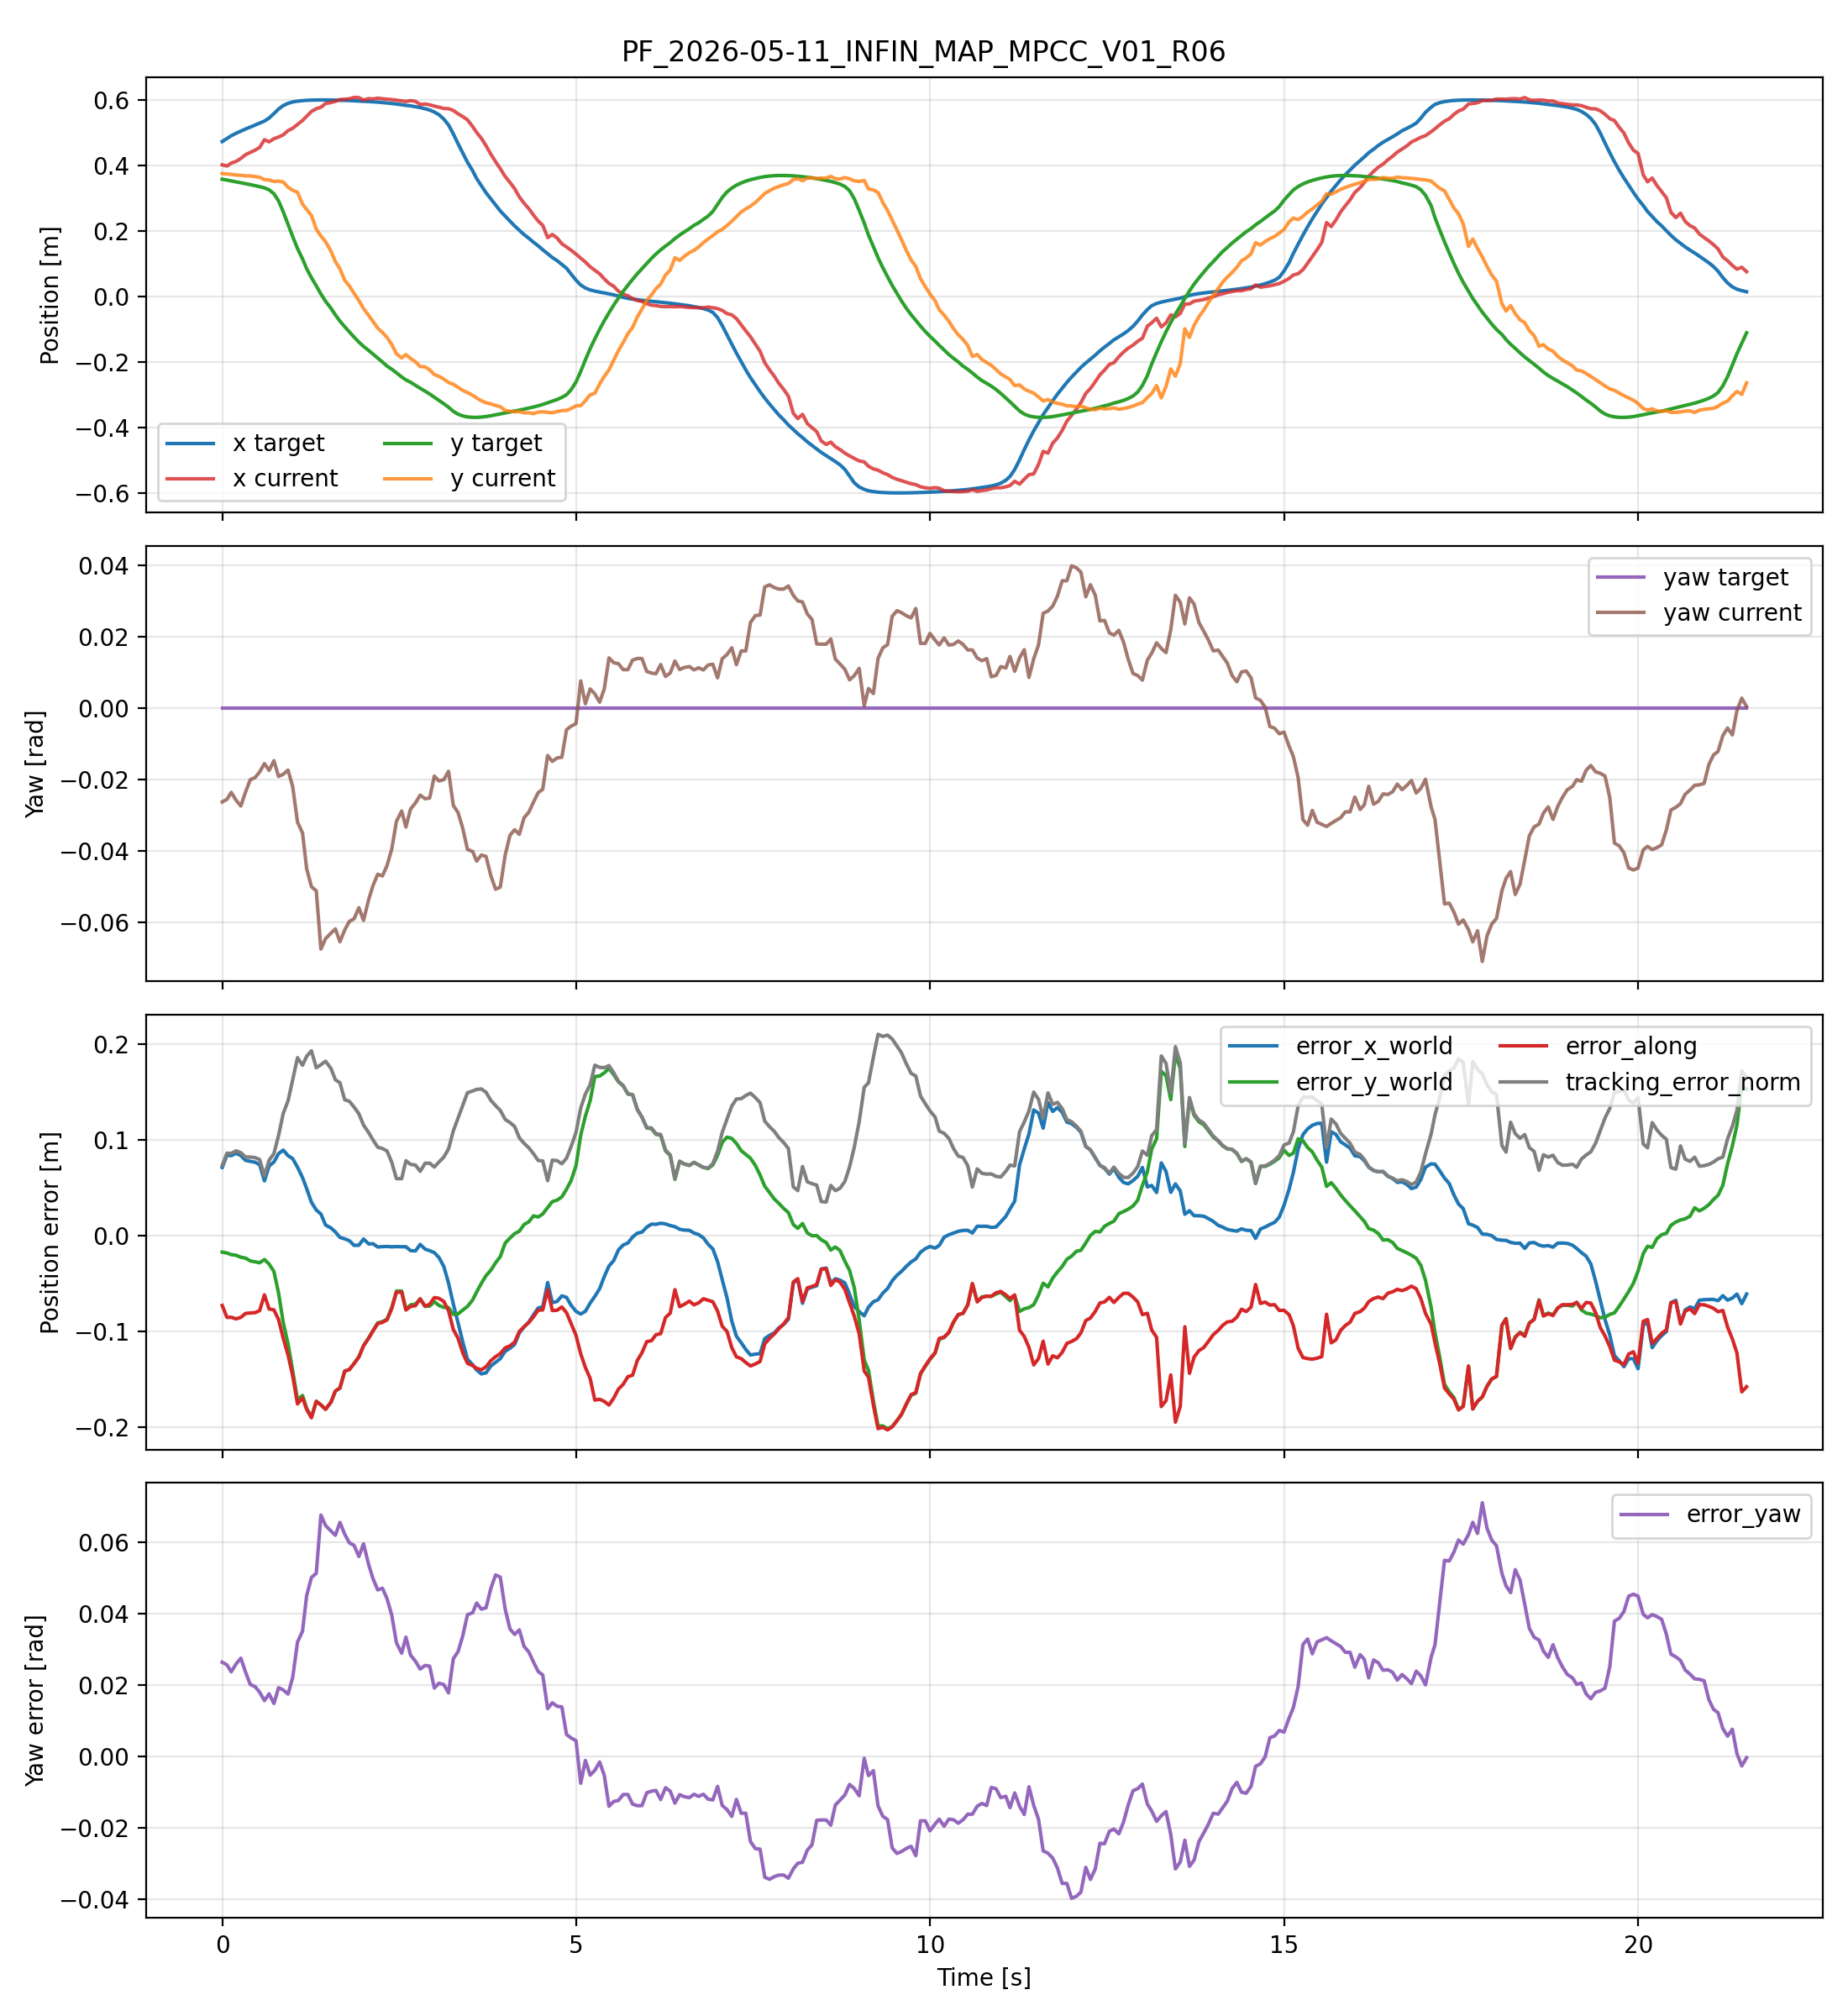
\includegraphics[width=0.7\linewidth]{IMG/controller/MPC/MPC_06_track_error.png}
        \caption{MPC\_06 tracking and errors}
        \label{fig:MPC_06_tracking_and_errors}
    \end{subfigure}
    \caption{Experimental results for MPC\_06 scenario.}
    \label{fig:MPC_06_general}
\end{figure}

\subsection{Comparison Between Linear Segment and MPCC}
  \label{subsec:common_segment_comparison}

  The previous tables evaluate each experiment over its full recorded duration.
  This is useful to understand whether a controller is able to complete the path,
  but it is not always the fairest way to compare tracking quality.  In fact, two
  tests may cover different portions of the infinity-shaped trajectory, and the
  tracking errors computed over the full run may therefore refer to different path
  segments.  For this reason, a final comparison was performed by evaluating each
  pair of tests only over the common portion of the path covered by both runs.

  The comparison was computed using the curvilinear coordinate \(\gamma\).  For a
  set of selected runs, the common interval is defined as:
  \begin{equation}
      \gamma_{\min}^{c}
      =
      \max_j \gamma_{\min,j},
      \qquad
      \gamma_{\max}^{c}
      =
      \min_j \gamma_{\max,j}.
  \end{equation}
  Only the samples satisfying
  \begin{equation}
      \gamma \in
      \left[
          \gamma_{\min}^{c},
          \gamma_{\max}^{c}
      \right]
  \end{equation}
  are used in the final comparison.  This makes the evaluation independent of the
  different total path progress reached by each controller.

  The error is not computed with respect to the internal target point published by
  each controller.  Instead, each measured robot position is compared with the same
  geometric reference path, interpolated at the recorded value of \(\gamma\).  Let
  \(\mathbf{p}=[x\;y]^T\) be the measured robot position and
  \(\mathbf{p}_r(\gamma)=[x_r(\gamma)\;y_r(\gamma)]^T\) the reference point on the
  path.  The position error is:
  \begin{equation}
      \mathbf{e}
      =
      \mathbf{p}
      -
      \mathbf{p}_r(\gamma).
  \end{equation}
  Using the local tangent and normal vectors:
  \begin{equation}
      \mathbf{t}(\gamma)
      =
      \begin{bmatrix}
          \cos\psi_r(\gamma) \\
          \sin\psi_r(\gamma)
      \end{bmatrix},
      \qquad
      \mathbf{n}(\gamma)
      =
      \begin{bmatrix}
          -\sin\psi_r(\gamma) \\
          \cos\psi_r(\gamma)
      \end{bmatrix},
  \end{equation}
  the error is decomposed into lag and contouring components:
  \begin{equation}
      e_l
      =
      \mathbf{e}^T \mathbf{t}(\gamma),
      \qquad
      e_c
      =
      \mathbf{e}^T \mathbf{n}(\gamma).
  \end{equation}
  The contouring error \(e_c\) measures the lateral distance from the path and is
  the most relevant quantity for geometric path-following accuracy.  The lag error
  \(e_l\) measures whether the robot is ahead of or behind the reference point
  along the path direction.  For this final comparison, the reported metrics are:
  \begin{equation}
      \mathrm{RMSE}_{e_c}
      =
      \sqrt{
          \frac{1}{N}
          \sum_{i=1}^{N} e_{c,i}^{2}
      },
      \qquad
      \mathrm{MAE}_{e_c}
      =
      \frac{1}{N}
      \sum_{i=1}^{N} |e_{c,i}|,
  \end{equation}
  \begin{equation}
      \max |e_c|
      =
      \max_{i=1,\dots,N} |e_{c,i}|,
      \qquad
      \mathrm{RMSE}_{e_l}
      =
      \sqrt{
          \frac{1}{N}
          \sum_{i=1}^{N} e_{l,i}^{2}
      },
      \qquad
      \mathrm{MAE}_{e_l}
      =
      \frac{1}{N}
      \sum_{i=1}^{N} |e_{l,i}|.
  \end{equation}
  The path progress ratio and the velocity saturation ratios are not included in
this final comparison, because the objective here is to isolate the tracking
quality on the same path segment.

\begin{table}[H]
\centering
\caption{Common-segment comparison between selected Linear Segment and MPCC
tests.}
\label{tab:common_segment_comparison}
\scriptsize
\setlength{\tabcolsep}{3pt}
\renewcommand{\arraystretch}{1.05}
\begin{tabular}{lccccccc}
\toprule
\textbf{Run} &
\shortstack{\textbf{Common}\\\textbf{segment [m]}} &
\textbf{Duration [s]} &
\(\mathrm{RMSE}_{e_c}\) [m] &
\(\mathrm{MAE}_{e_c}\) [m] &
\(\max |e_c|\) [m] &
\(\mathrm{RMSE}_{e_l}\) [m] &
\(\mathrm{MAE}_{e_l}\) [m] \\
\midrule
LIN-04 & 4.548 & 50.14 & 0.0115 & 0.0086 & 0.0367 & 0.0003 & 0.0002 \\
LIN-05 & 4.548 & 38.86 & 0.0259 & 0.0210 & 0.0646 & 0.0010 & 0.0005 \\
\midrule
MPC-05 & 4.534 & 35.39 & 0.0170 & 0.0144 & 0.0357 & 0.0666 & 0.0587 \\
MPC-06 & 4.534 & 21.53 & 0.0330 & 0.0257 & 0.0705 & 0.1105 & 0.1039 \\
\midrule
LIN-05 & 4.534 & 22.58 & 0.0469 & 0.0391 & 0.1166 & 0.0011 & 0.0006 \\
MPC-06 & 4.534 & 21.53 & 0.0330 & 0.0257 & 0.0705 & 0.1105 & 0.1039 \\
\bottomrule
\end{tabular}
\end{table}

The first comparison considers two Linear Segment runs. The slower configuration
LIN-R05 achieves the best contouring performance. Increasing the velocity in
LIN-R06 reduces the duration from \(50.14~\mathrm{s}\) to
\(38.86~\mathrm{s}\), but the maximum contouring error increases from
\(0.0367~\mathrm{m}\) to \(0.0646~\mathrm{m}\), which is almost doubled.
This confirms that the Linear Segment controller is very accurate at moderate
speed, but its lateral tracking quality degrades as the motion becomes more
aggressive.

The second comparison considers two MPCC runs. MPC-R05 provides better geometric
tracking, with \(\mathrm{RMSE}_{e_c}=0.0170~\mathrm{m}\) and
\(\max |e_c|=0.0357~\mathrm{m}\). MPC-R06 is faster, completing the common
segment in \(21.53~\mathrm{s}\), but the contouring error increases to
\(\mathrm{RMSE}_{e_c}=0.0330~\mathrm{m}\), with a maximum contouring error of
\(0.0705~\mathrm{m}\). The lag error also increases significantly, from
\(\mathrm{RMSE}_{e_l}=0.0666~\mathrm{m}\) to
\(\mathrm{RMSE}_{e_l}=0.1105~\mathrm{m}\). This indicates that the aggressive
MPCC configuration favours path advancement, but introduces a larger mismatch
between the robot motion and the virtual path coordinate.

The final cross-comparison evaluates the aggressive Linear Segment run LIN-R10
against MPC-R06 over the same \(4.534~\mathrm{m}\) common segment. In this case,
MPC-R06 achieves better lateral path-following accuracy:
\[
    \mathrm{RMSE}_{e_c}
    =
    0.0330~\mathrm{m}
    \quad \text{against} \quad
    0.0469~\mathrm{m}
\]
for LIN-R10. The maximum contouring error is also lower for MPC-R06:
\[
    \max |e_c|
    =
    0.0705~\mathrm{m}
    \quad \text{against} \quad
    0.1166~\mathrm{m}.
\]
However, the lag error remains much larger for MPC-R06
\((\mathrm{RMSE}_{e_l}=0.1105~\mathrm{m})\) than for the Linear Segment
controller \((\mathrm{RMSE}_{e_l}=0.0011~\mathrm{m})\). Therefore, the MPCC
shows better lateral geometric tracking in the aggressive comparison, but still
requires further tuning of the lag penalty and path advancement dynamics. The
Linear Segment controller remains simpler and very effective when its velocity
is moderate, while the MPCC becomes more promising when higher-speed geometric
path following is required.

  \begin{figure}[H]
      \centering
      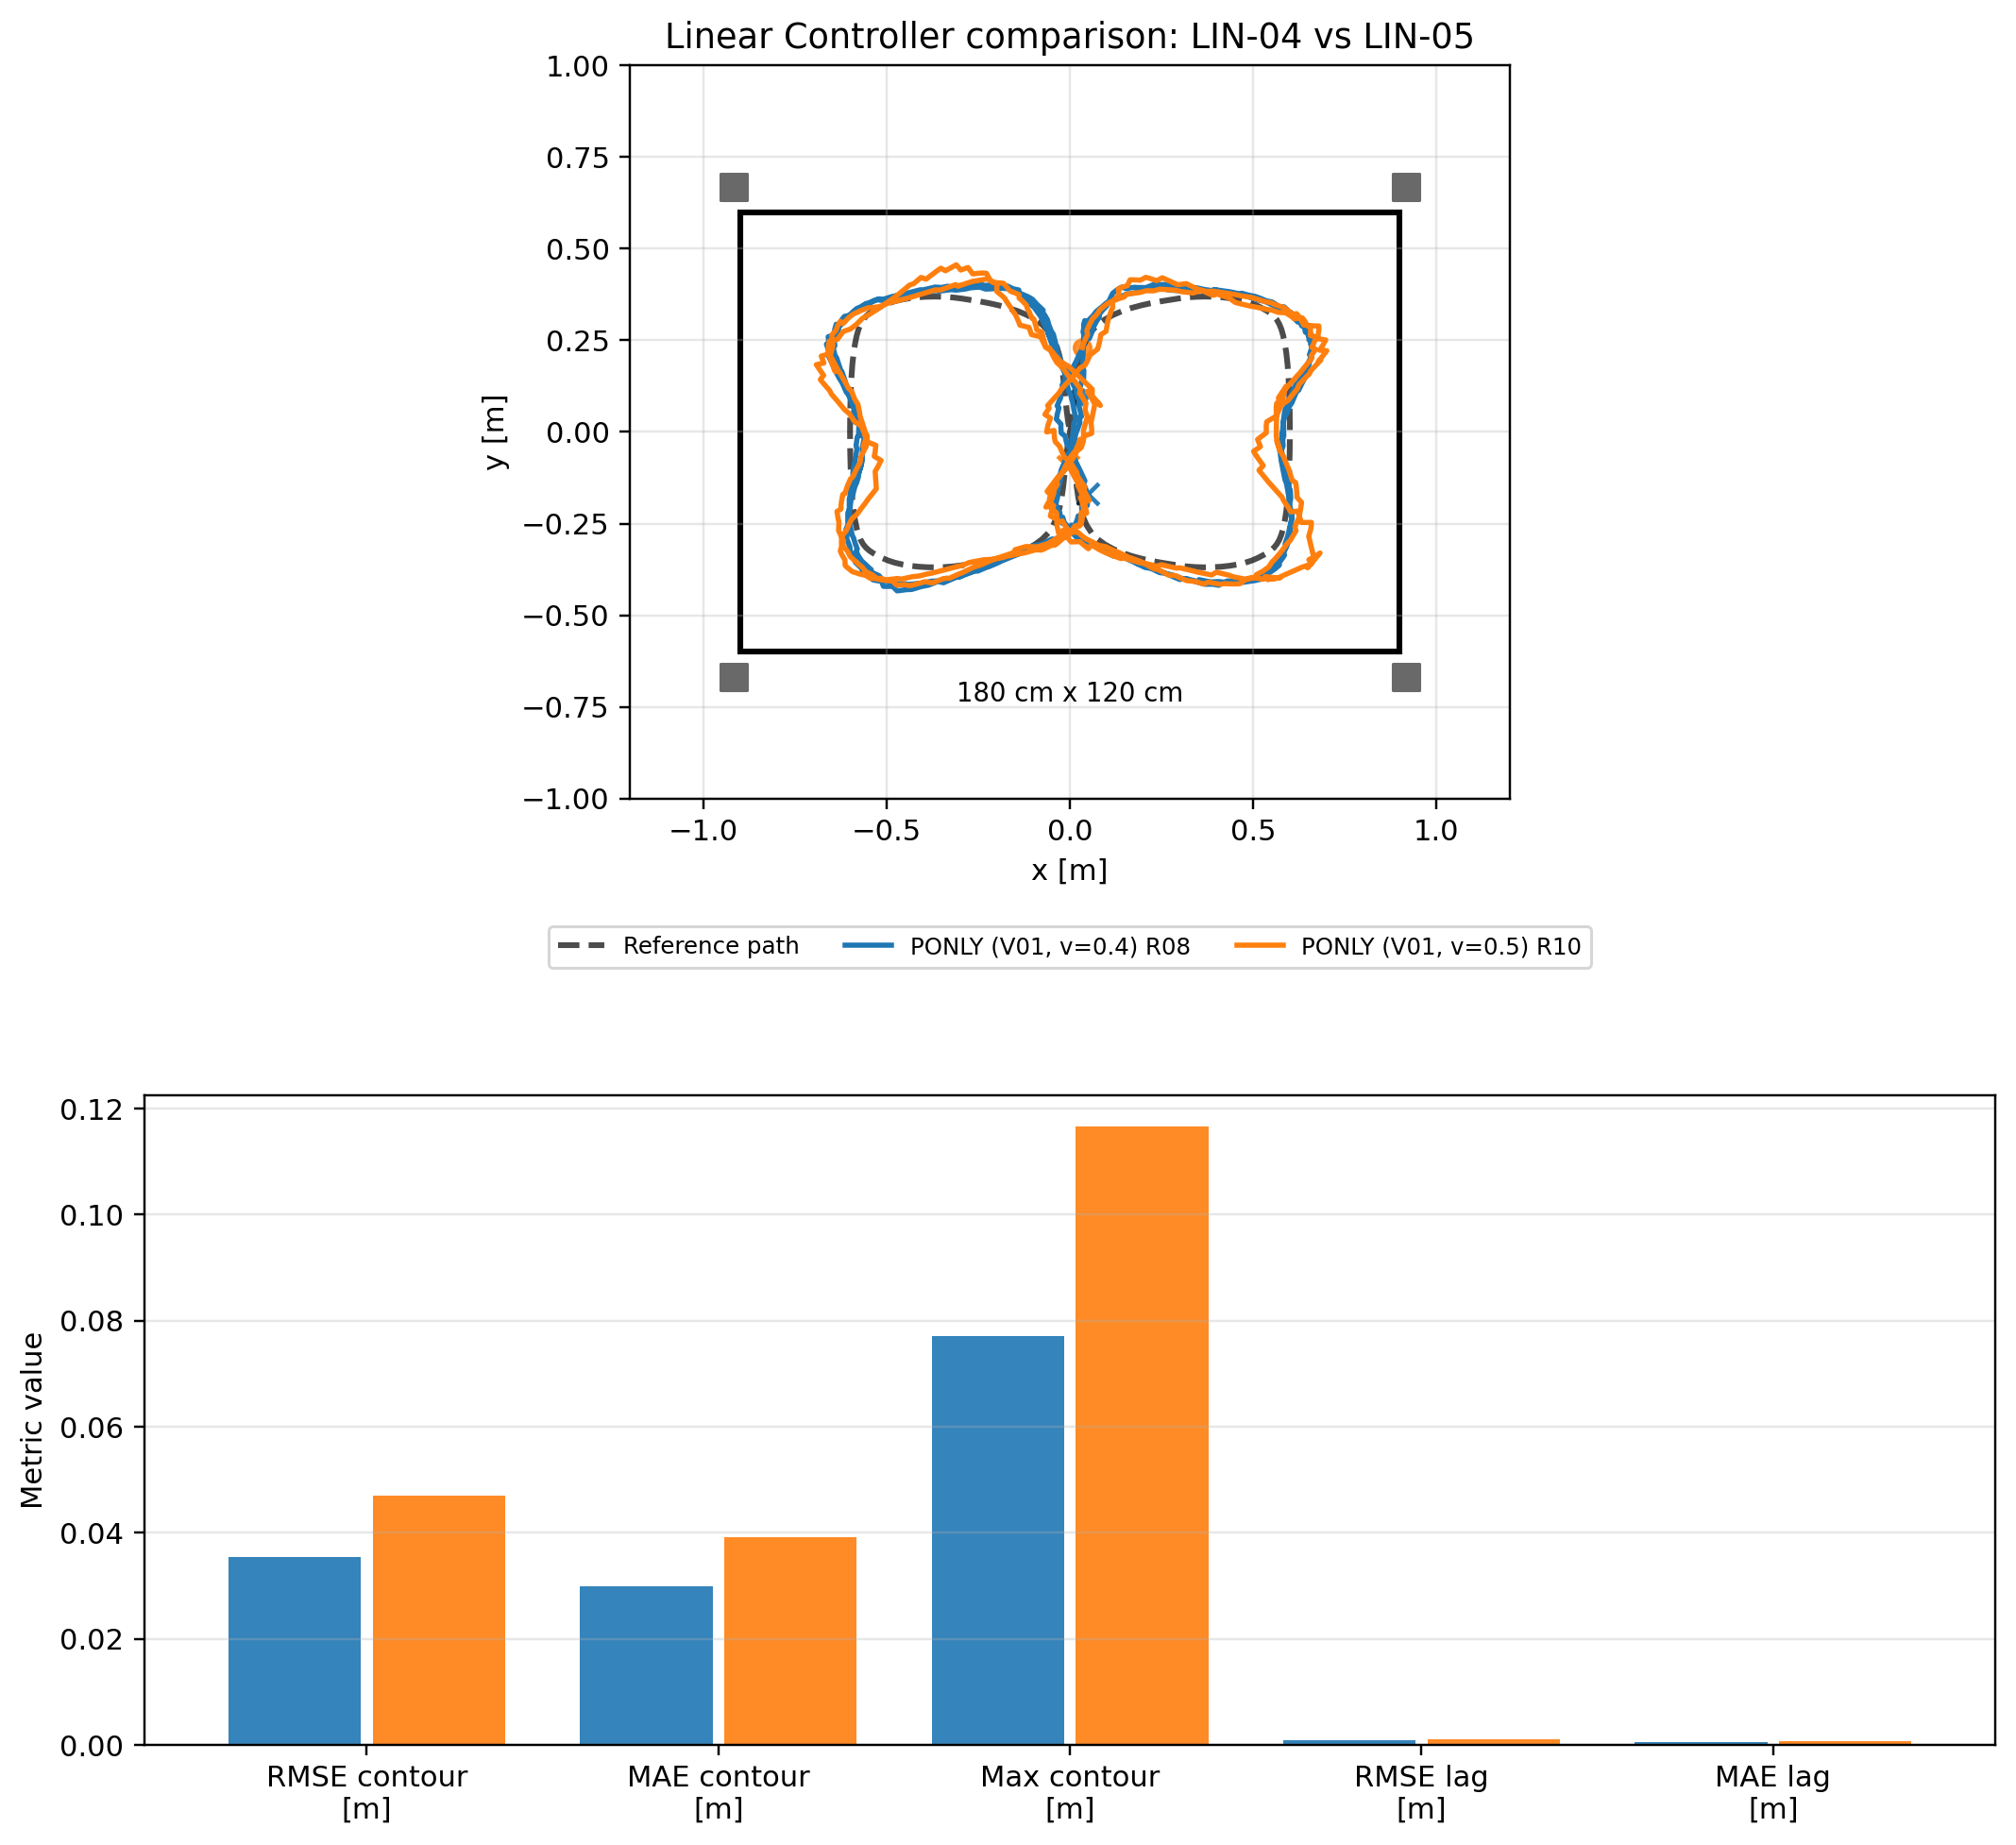
\includegraphics[width=0.95\linewidth]{IMG/controller/COMPARISON/compare_LIN05_LIN06.png}
      \caption{Common-segment comparison between two Linear Segment runs.  The
  upper plot shows the overlapped \(xy\) trajectories, while the lower plot reports
  the contouring and lag error metrics.}
      \label{fig:compare_lin05_lin06}
  \end{figure}

  \begin{figure}[H]
      \centering
      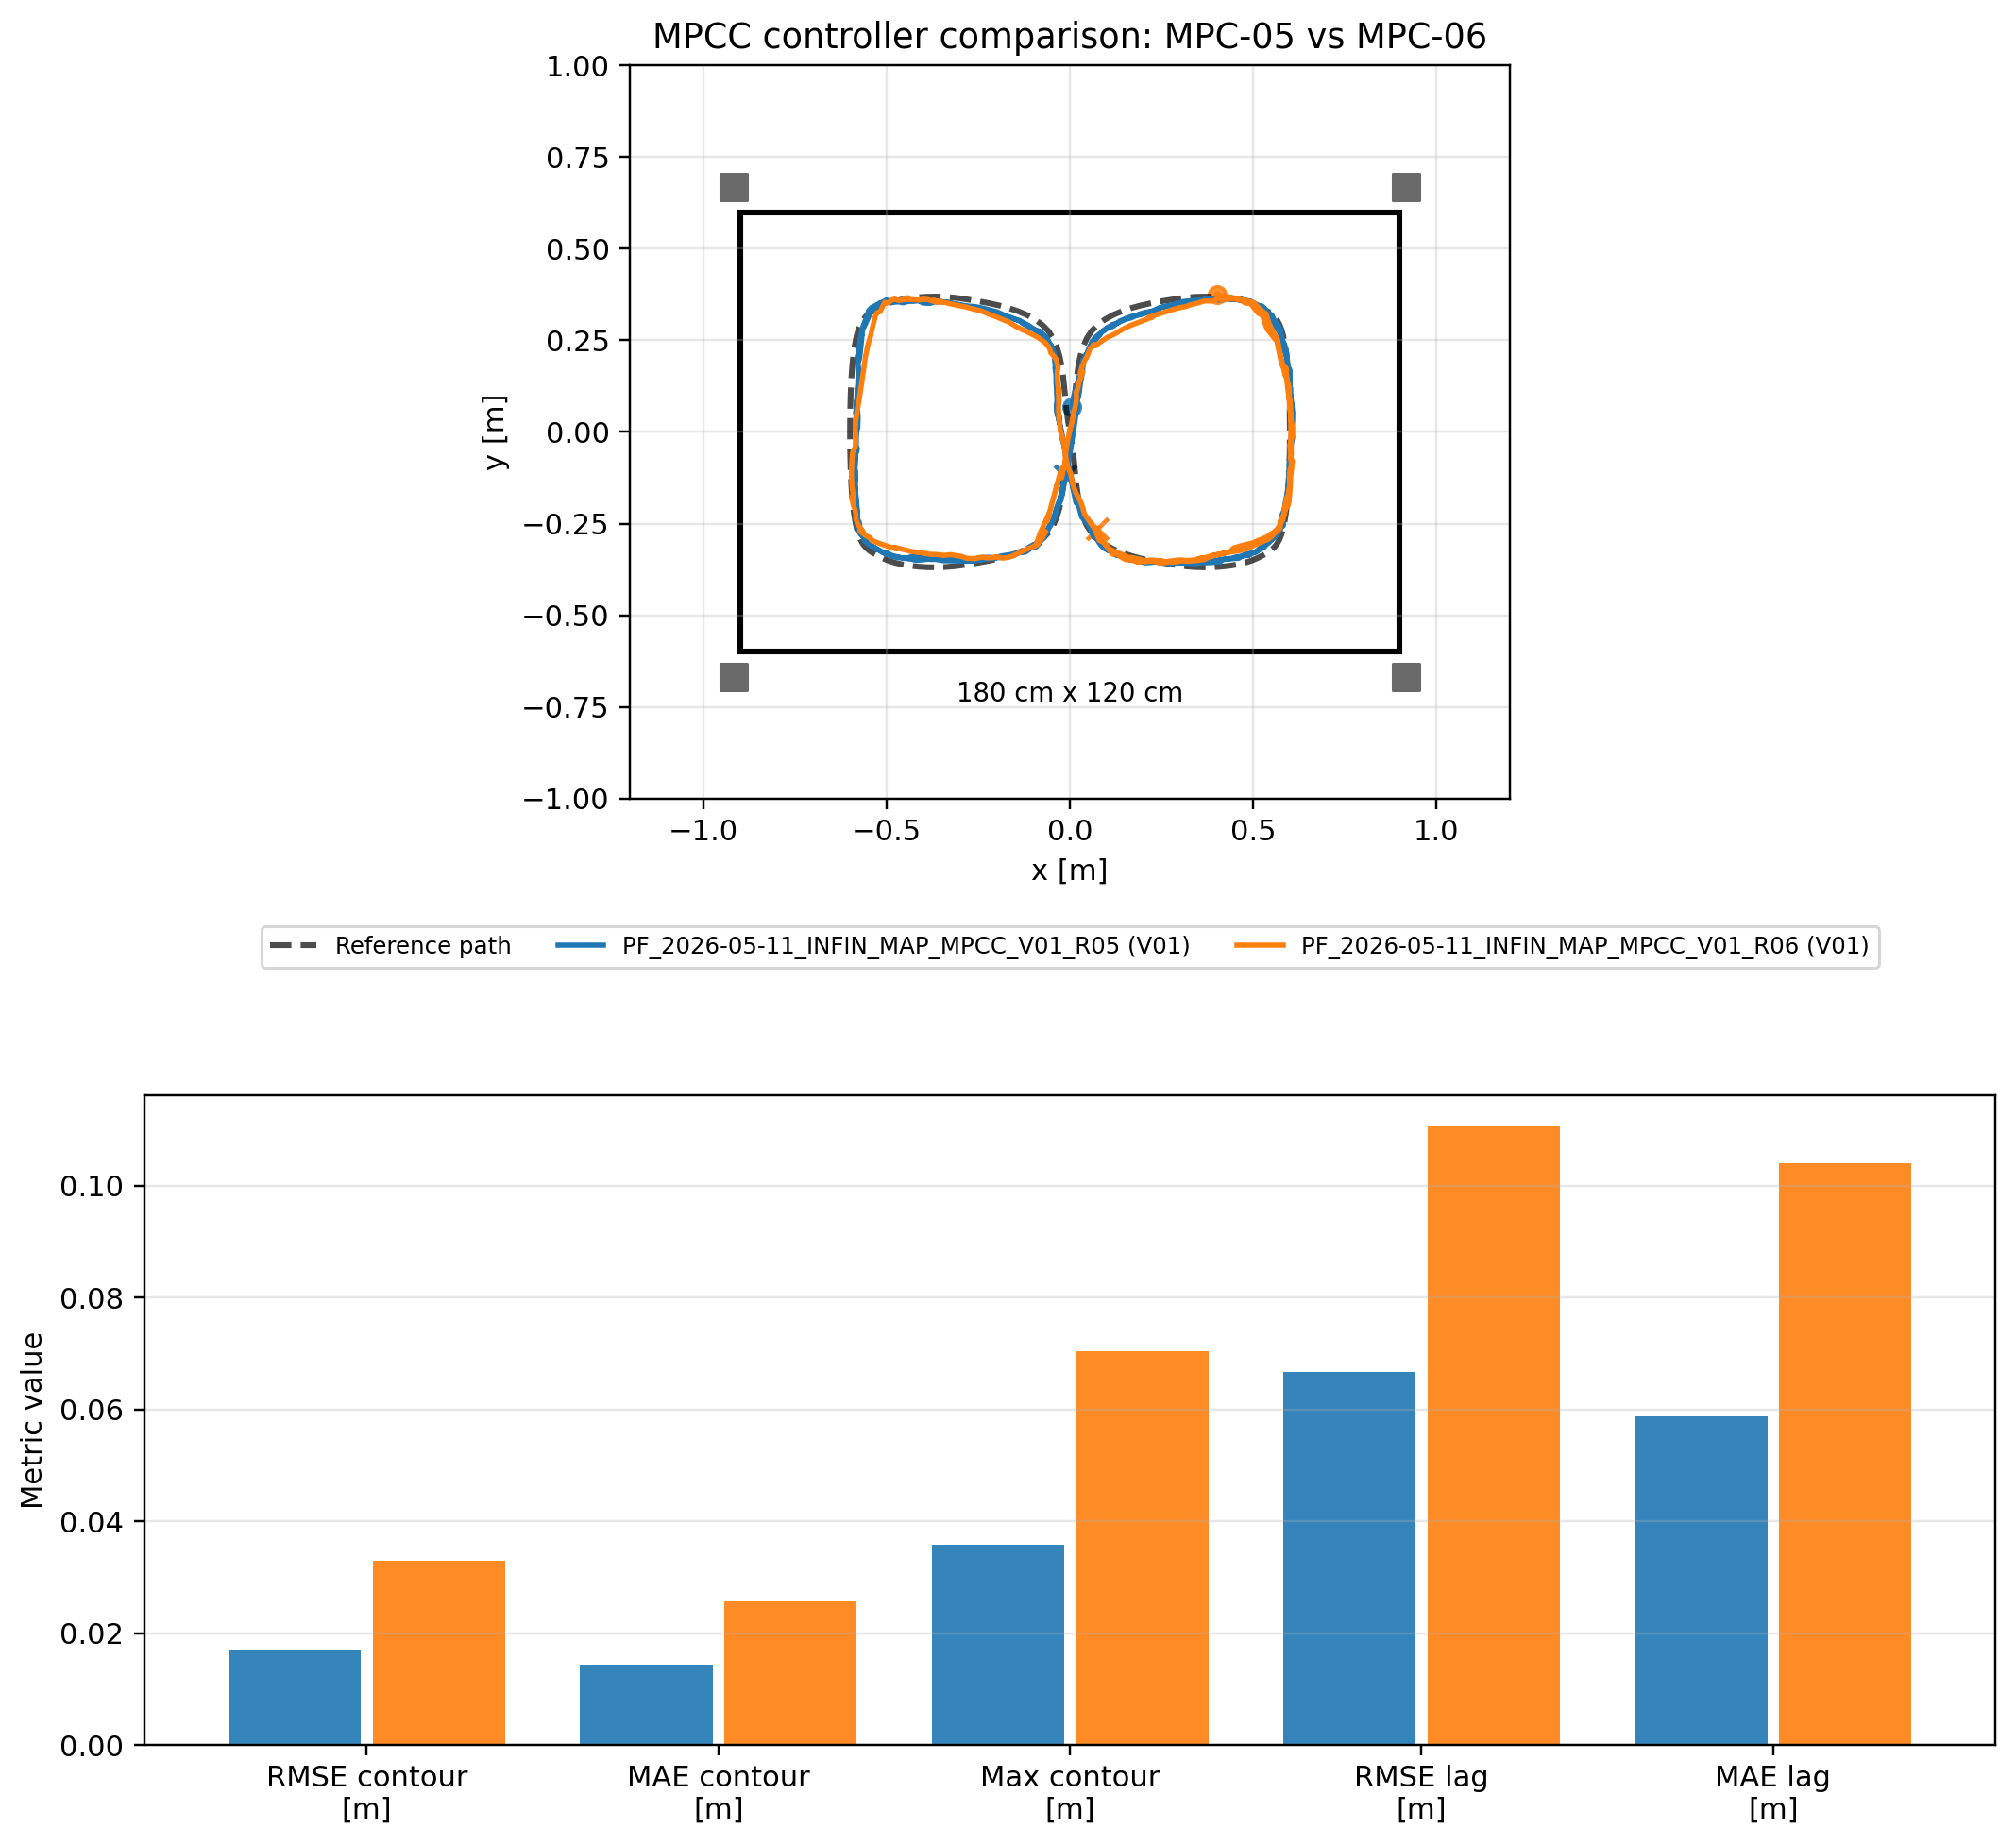
\includegraphics[width=0.95\linewidth]{IMG/controller/COMPARISON/compare_MPC05_MPC06.png}
      \caption{Common-segment comparison between two MPCC runs.  The figure
  highlights the loss of contouring accuracy and the increase in lag error when
  moving from MPC-05 to the more aggressive MPC-06 configuration.}
      \label{fig:compare_mpc05_mpc06}
  \end{figure}

\begin{figure}[H]
    \centering
    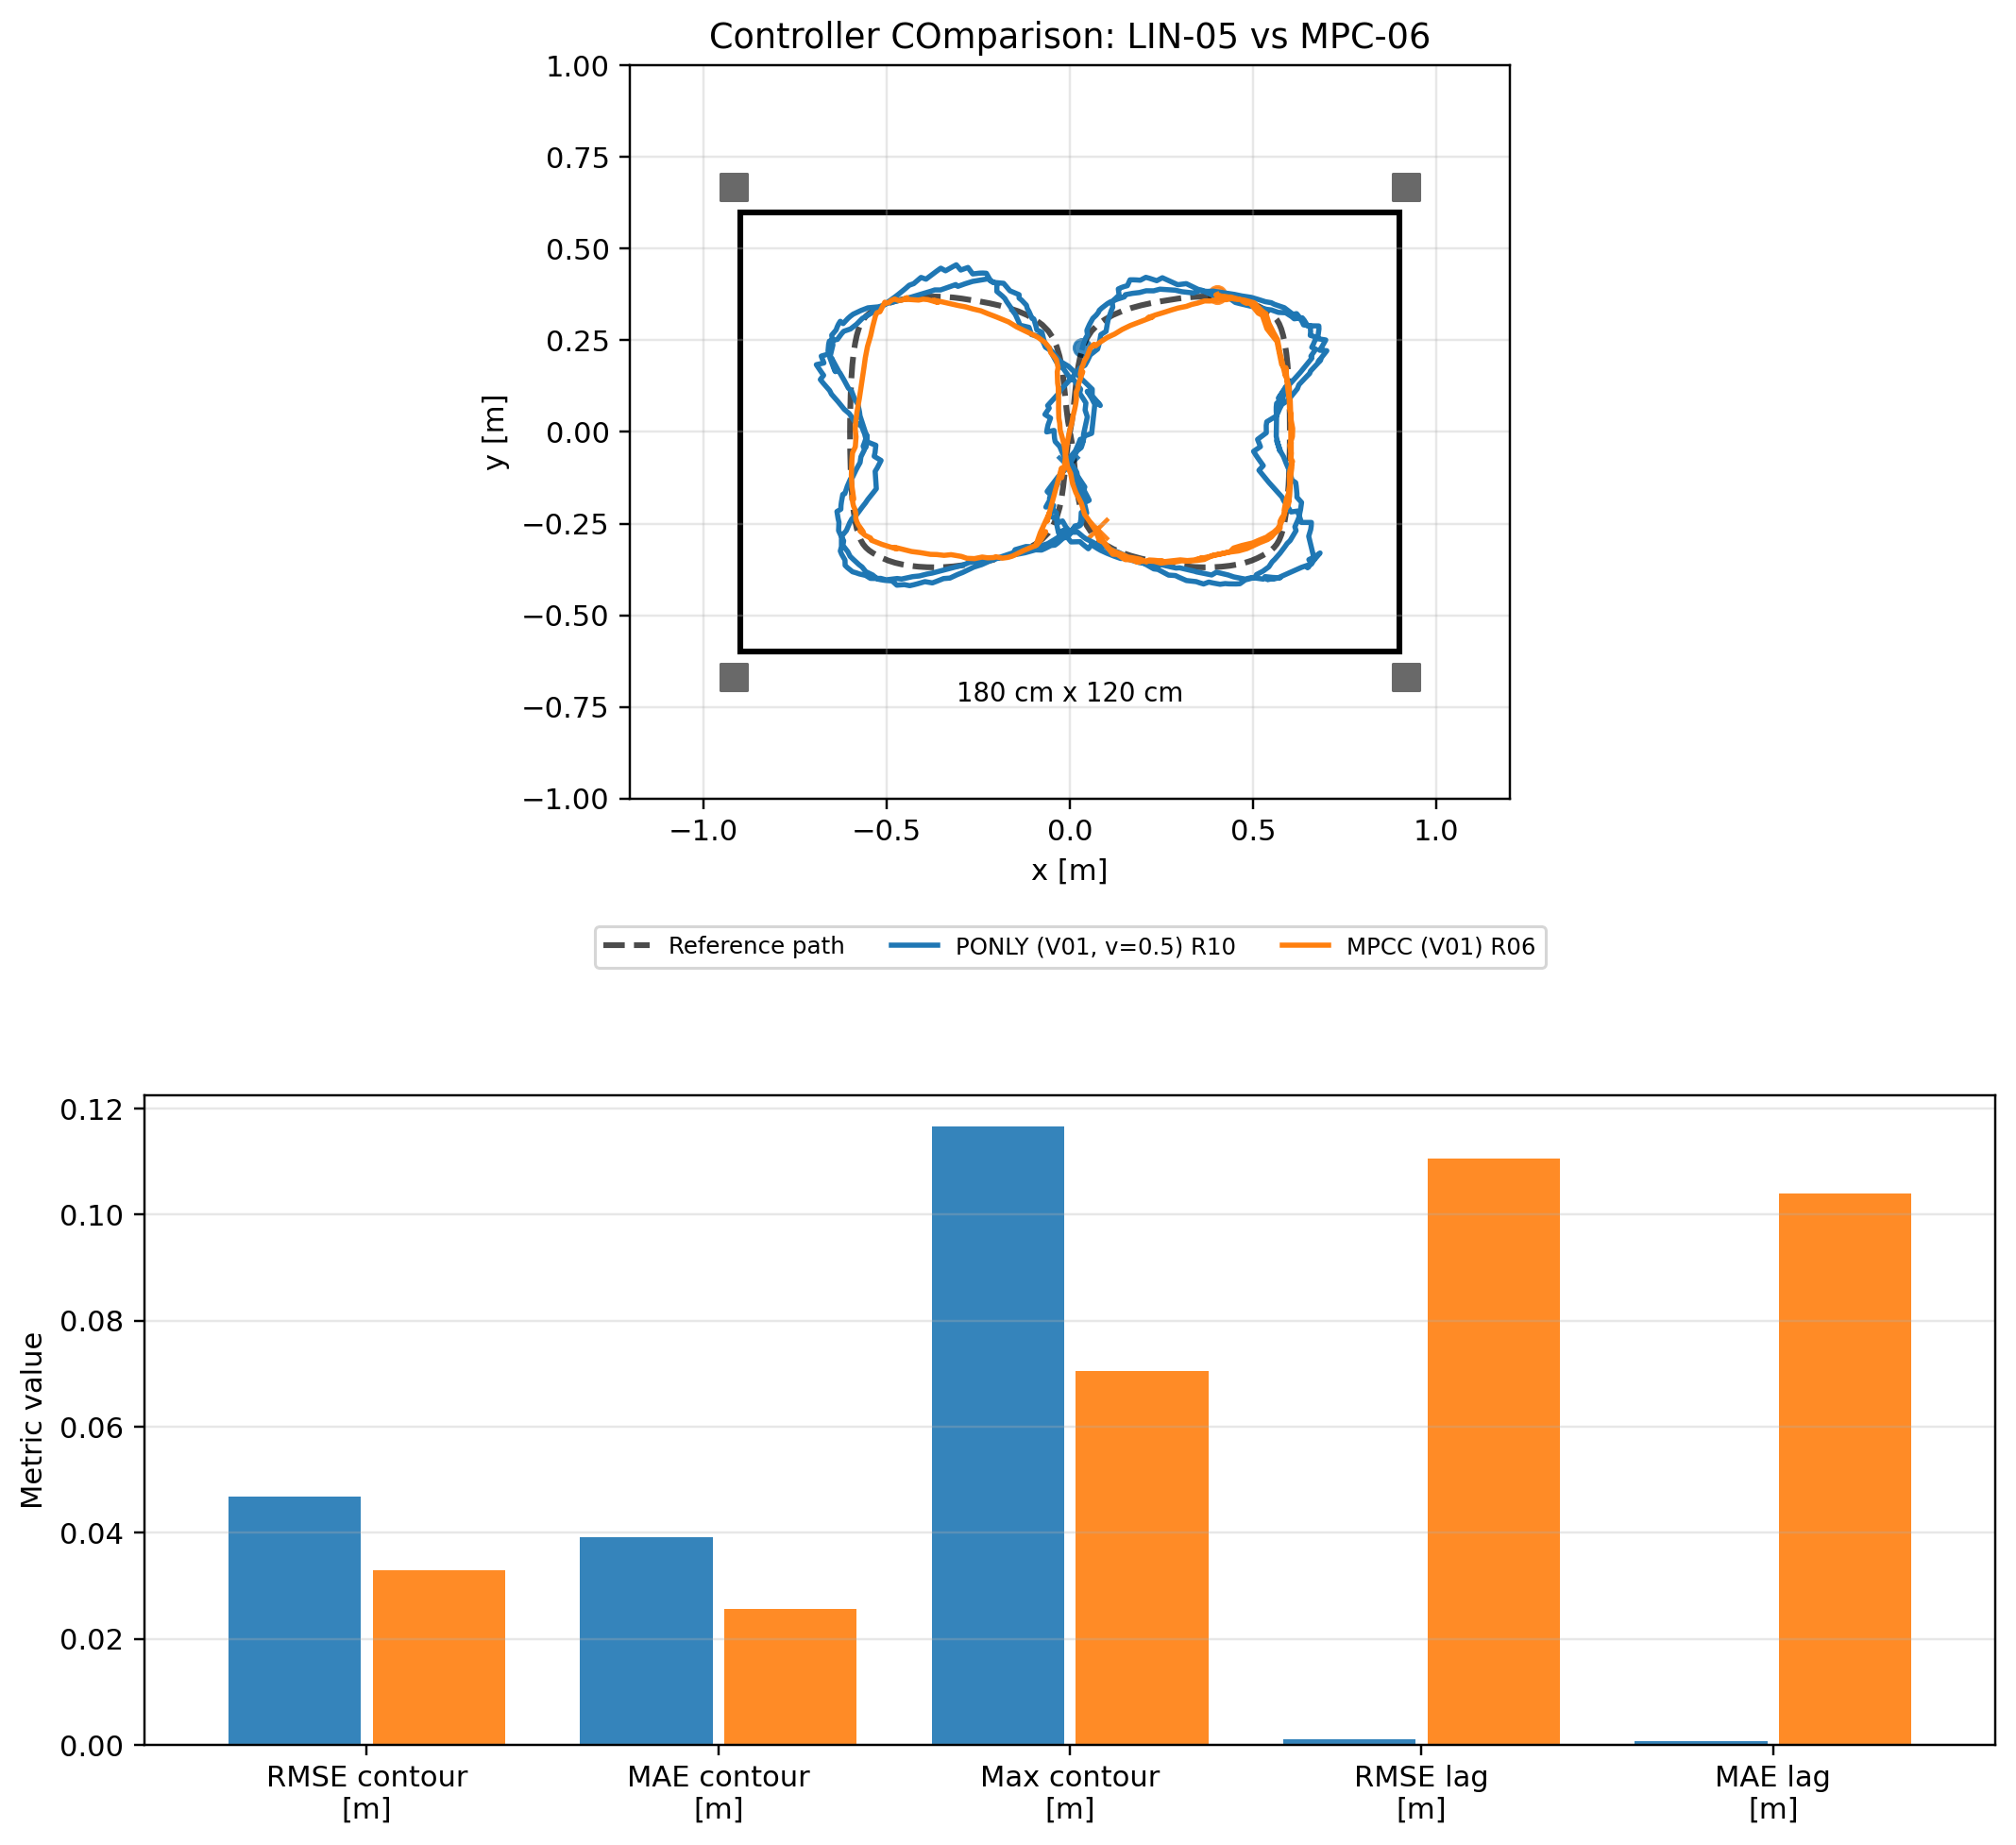
\includegraphics[width=0.95\linewidth]{IMG/controller/COMPARISON/compare_LIN05_MPC06.png}
    \caption{Common-segment comparison between the aggressive Linear Segment run
LIN-R10 and the aggressive MPCC run MPC-R06. MPC-R06 reduces the contouring error
but presents a larger lag error.}
    \label{fig:compare_lin10_mpc06}
\end{figure}
